\documentclass[twoside,a4paper,12pt]{article}
%\usepackage[applemac]{inputenc}
\usepackage{wrapfig}
\usepackage{graphicx}
\usepackage{graphics}
%\usepackage{subfig}
%\usepackage{inputenc}
\usepackage{amsmath}
\usepackage{amsfonts}
\usepackage{amssymb}
\usepackage[singlelinecheck=false]{caption}
\usepackage{array}
\usepackage{multirow}
\usepackage{setspace}
\usepackage{hyperref}
\usepackage{verbatim}
\usepackage[clearempty]{titlesec}
\usepackage{epstopdf}
\usepackage{textcomp}
\usepackage{nicefrac}
\usepackage{xspace}
%\usepackage{autoref}
\usepackage[small, bf, hang, raggedright]{subfigure}

\usepackage[english]{babel} 

\onehalfspacing
\usepackage[left=2.9cm,right=2.9cm,top=3cm,bottom=4.5cm]{geometry}
\newcommand\leerseite{\newpage\thispagestyle{empty}\hspace{1cm}\newpage}

\newcommand{\subfigureautorefname}{\figurename}

\newcommand\piminus{\(\mathrm{\pi^-}\)}
\newcommand\muminus{\(\mathrm{\mu^-}\)}
\newcommand\eminus{\(\mathrm{e^-}\)}
\newcommand\eplus{\(\mathrm{e^+}\)}
\newcommand\geant{\textsc{Geant\,4}\xspace}

\begin{document}\selectlanguage{english}
\begin{titlepage}
\begin{flushright}
CALICE Analysis Note CAN-056\\
v1.6\\
May 12, 2016 \\
\end{flushright}

\begin{center}
\vspace*{\fill}
\begin{LARGE} \textbf{Pion Response and Resolution in a Combined Scintillator Calorimeter System in the FNAL Testbeam} \end{LARGE} \\ [10ex]
\begin{Large} The CALICE Collaboration \footnote{Corresponding author: \\ Oskar Hartbrich; oskar.hartbrich@desy.de}\\ [10ex] 
\end{Large}
\begin{large}
\textbf{Abstract} \\
\end{large}
\end{center}
This note presents results obtained with the combined scintillator-SiPM calorimeter system consisting of the \emph{Scintillator Electromagnetic Calorimeter}, \emph{Analogue Hadronic Calorimeter} and \emph{Tail Catcher \& Muon Tracker} in the energy range 4--32\,GeV at the FNAL testbeam campaign in 2009. The analysis includes longitudinal profiles as well as response linearity and energy resolution of pions for standard and software compensation reconstruction. The results are compared to several \geant physics lists in software versions 9.6 and 10.1.\\
\\

\textit{
This note contains preliminary CALICE results, and is for the use of members of the CALICE Collaboration and others to whom permission has been given.}

\end{titlepage}

\clearpage
\tableofcontents
\newpage
\section{Introduction}
$\alpha_i, \beta_i$ as well as the TCMT weight $\gamma$
Experiments at future \eplus\eminus colliders require unprecedented jet energy resolutions of 3--4\% across the full expected energy range. One concept to achieve such resolutions is \emph{Particle Flow Algorithms} (PFAs) aiming to combine measurements from the tracking system with calorimeter depositions, which needs exceptional granularity in the calorimeters. The CALICE collaboration develops, builds and tests different calorimeters that aim to fulfill the requirements for ideal application of PFAs.

One explored option consists of scintillator tiles or strips of a few cm${}^2$ size, read out by one individual \emph{Silicon Photomultiplier} (SiPM) per cell. Several prototypes with different absorbers, granularities and sampling structures have been constructed.  

In a common beamtest at FNAL in 2009 the \emph{Scintillator Electromagnetic Calorimeter} (ScECAL), \emph{Analogue Hadronic Calorimeter} (AHCAL) and \emph{Tail Catcher \& Muon Tracker} (TCMT) have been operated as a combined scintillator-SiPM calorimeter system in beams of muons, electrons and pions in the energy range 1--32\,GeV. Studying the characteristics of single pion events is of special interest, as they can deposit significant amounts of energy in all detector parts and their calorimetric energy resolution is a significant contribution to the expected achievable PFA performance. 

Apart from PFA reconstruction, the high granularity of the used calorimeters on the scale of electromagnetic shower development ($\approx1\,X_0$ longitudinal sampling, $\approx1\,r_M$ transverse segmentation) enables the identification of electromagnetic sub-showers within hadron showers and thus the application of software compensation techniques to improve the energy resolution of the calorimeter system. 

This note presents results obtained from the FNAL 2009 testbeam, combining depositions in the ScECAL, AHCAL and the first eight layers of TCMT.% Section 2 describes the experimental setup at FNAL. The reworked MC model of the ScECAL and its validation with electromagnetic showers is described in Section 3. Section 4 lists the data runs and simulations used for the analysis as well as selections performed on these datasets to obtain clean samples of single pion events. The techniques used to reconstruct the energy of an incoming particle from the depositions in the calorimeters are discussed in Section 5. Single pion results obtained from the testbeam data as well as simulations are compared in Section 6.


\section{The FNAL 2009 Testbeam Setup}
The data sets used in this note were acquired during a testbeam campaign in May 2009 at the Fermilab Testbeam Facility (FTBF). Its MTest beamline delivers secondary particle beams with particle momenta in the range 1--32\,GeV. The beamline is equipped with a two channel differential gas Cherenkov counter as well as various scintillator triggers. The calorimeter prototypes are installed in the order ScECAL, AHCAL, TCMT downstream of the beam instrumentation. More detailed descriptions of the beamline setup are available in \cite{Feege, CAN16}.

One ScECAL layer consists of 3.5\,mm W-based absorber and 72 scintillator strips of $10\times45\times3\,\text{mm}^3$ each for a total area of $18\times18\,\text{cm}^3$. 30 layers are stacked for a depth of around $20X_0$ ($\approx 1\,\lambda_\text{n}$) and 2160 channels total \cite{CAN16}.
The AHCAL is a $1\times1\times1\,\text{m}^3$ calorimeter prototype with Fe absorber plates, instrumented with 7608 5\,mm thick scintillator tiles of size $3\times3\,\text{cm}^2$--$12\times12\,\text{cm}^2$ in 38 layers for a full depth of 5.3 nuclear interaction lengths $\lambda_\text{n}$ \cite{CommPaper}. The TCMT covers $1\times1\,\text{m}^2$ Fe absorber plates with a total of 320 scintillator strips of $5\times100\,\text{cm}^2$ each in 16 layers, instrumenting a depth of 5.2\,$\lambda_\text{n}$ \cite{TCMTPaper}.

 



\section{Simulation}
%The simulation uses Mokka detector model \emph{TBFnal0508}, including basic trigger scintillators but no further detailled beam instrumentation. The detector models used for each subdetector are \emph{TBscint04} for the ScECAL, \emph{TBhcal08} for the AHCAL and \emph{TBcatcher08} for the TCMT.
The simulation models for AHCAL and TCMT are used as in \cite{Feege, Guenter}, the ScECAL is described in the next section. 
The right handed coordinate system is laid out such that the Z-axis is pointing in the beam direction and the Y-axis is pointing upwards. 

Depending on the pressure in the Cherenkov gas tube, the material between final beam energy selection magnet and calorimeter front face amounts to 0.08-0.16\,$X_0$ distributed over around 30\,m as estimated in \cite{Feege}.
As the helium filled beam transport tubes and most of the beam instrumentation is not represented in the simulation model, a similar amount of material between beam generation and calorimeter front face is achieved by filling the world volume with air, setting the beam gun at 6\,m from the calorimeter front face and adding 5\,mm of Al directly in front of the ScECAL, amounting to around 0.1\,$X_0$ in total. The beam momentum spread is set to 2.7\% for runs with beam energy $\leq$4\,GeV and 2.3\% for runs with higher beam energies following \cite{CAN16b}. The beam profile is extracted from data and transferred into the simulation for each run individually. 

All simulated electron shower events in this note are produced with the QGSP\_BERT physics list in \geant 10.1p2, as no significant differences have been found to any other tested physics list. Pion showers are simulated using QGSP\_BERT\_HP in \geant 10.1p2 as well as FTFP\_BERT\_HP in \geant versions 10.1p2 and 9.6p3. Per simulated run 100,000 single particle events are generated.

\subsection{ScECAL Simulation Model \& Digitisation}
The ScECAL simulation model is constructed out of 30 single layers. Each logical layer is primarily composed of 3.5\,mm absorber plate, 3\,mm scintillator tile, 1\,mm PCB and 1.24\,mm air. The thicknesses of absorber, scintillator and PCB were measured precisely. The depth of air between layers follows from the measured total length of the ScECAL \cite{CAN16}. Density and material composition of scintillator and PCB are taken as the defaults for polystyrene and G10 in \geant. X-Ray diffraction (XRD) measurements show that the ScECAL absorber plates consist of WC (tungsten carbide) and Co, possibly a negligible amount of Cr, but no significant amount of elementary W \cite{ScECALAbsorber}. Assuming no air or vacuum bubbles, as supported by microscopic scale back scattered electron imaging (BSEI), the composition of the absorber plates can thus be calculated from its measured density and the known densities of WC and Co to be 74.6\% W, 4.9\% C and 20.5\% Co in mass fractions.

The digitisation of simulated hits closely resembles the AHCAL algorithm described in \cite{EMPaper}, using (where available) individual calibration factors per channel obtained from data to extract the light yield which is needed to model the statistical fluctuations of photons hitting the SiPM. Saturation effects are included in the same way, but only one global parameter is available for all cells (see \autoref{sec:scecalvalidation}). Since each scintillator strip in the ScECAL is individually wrapped in reflective foil, optical crosstalk effects between channels are assumed to be negligible and thus not included. Noise is extracted from random trigger events for each data run and overlaid onto simulated events. After the digitisation all simulated hits have the same format as raw data hits and are reconstructed with the same software chain that is used for data. The relative alignment between ScECAL and AHCAL is determined from data using tracks extracted from muon runs. To suppress noise hits, only hits above 0.5\,MIP are considered in the analysis in both data and simulation. 
\subsection{ScECAL Model Validation}\label{sec:scecalvalidation}
To validate the simulation and digitisation model described above, comparisons of electromagnetic interactions within the ScECAL are preferred as such interactions should be well described in simulations. 

One of the lowest level observables to compare is the spectrum of a MIP-like particle traversing a scintillator strip. A sample of such hits is obtained from straight tracks by muons and pions punching through the whole ScECAL without a hard interaction. The comparison for a single ScECAL strip in \autoref{fig:MIPspectrum} shows that the shape of the hit energy spectrum is well described in the digitised simulation. Fitting these spectra for all strips and extracting the most probable value yields the distribution in \autoref{fig:MIPmpv}. The mean of the distribution for both data and simulation is very close to unity. The width of the data distribution is slightly higher than in simulation, as channel-wise miscalibrations are not included in the digitisation.
% \begin{figure}[htbp]
% \begin{center}
% \includegraphics[width=0.8\textwidth]{fig/electron/mipspectrum_single_k08_ecal_560474.pdf}
% \caption{Hit energy spectrum of a single scintillator strip in run 560474 (32\,GeV \piminus) from MIP-like particle tracks in the ScECAL for data and simulation (QGSP\_BERT\_HP, \geant 10.1p2). }
% \label{fig:MIP}
% \end{center}
% \end{figure}

\begin{figure}[htbp]
	\subfigure[MIP Spectrum\label{fig:MIPspectrum}] {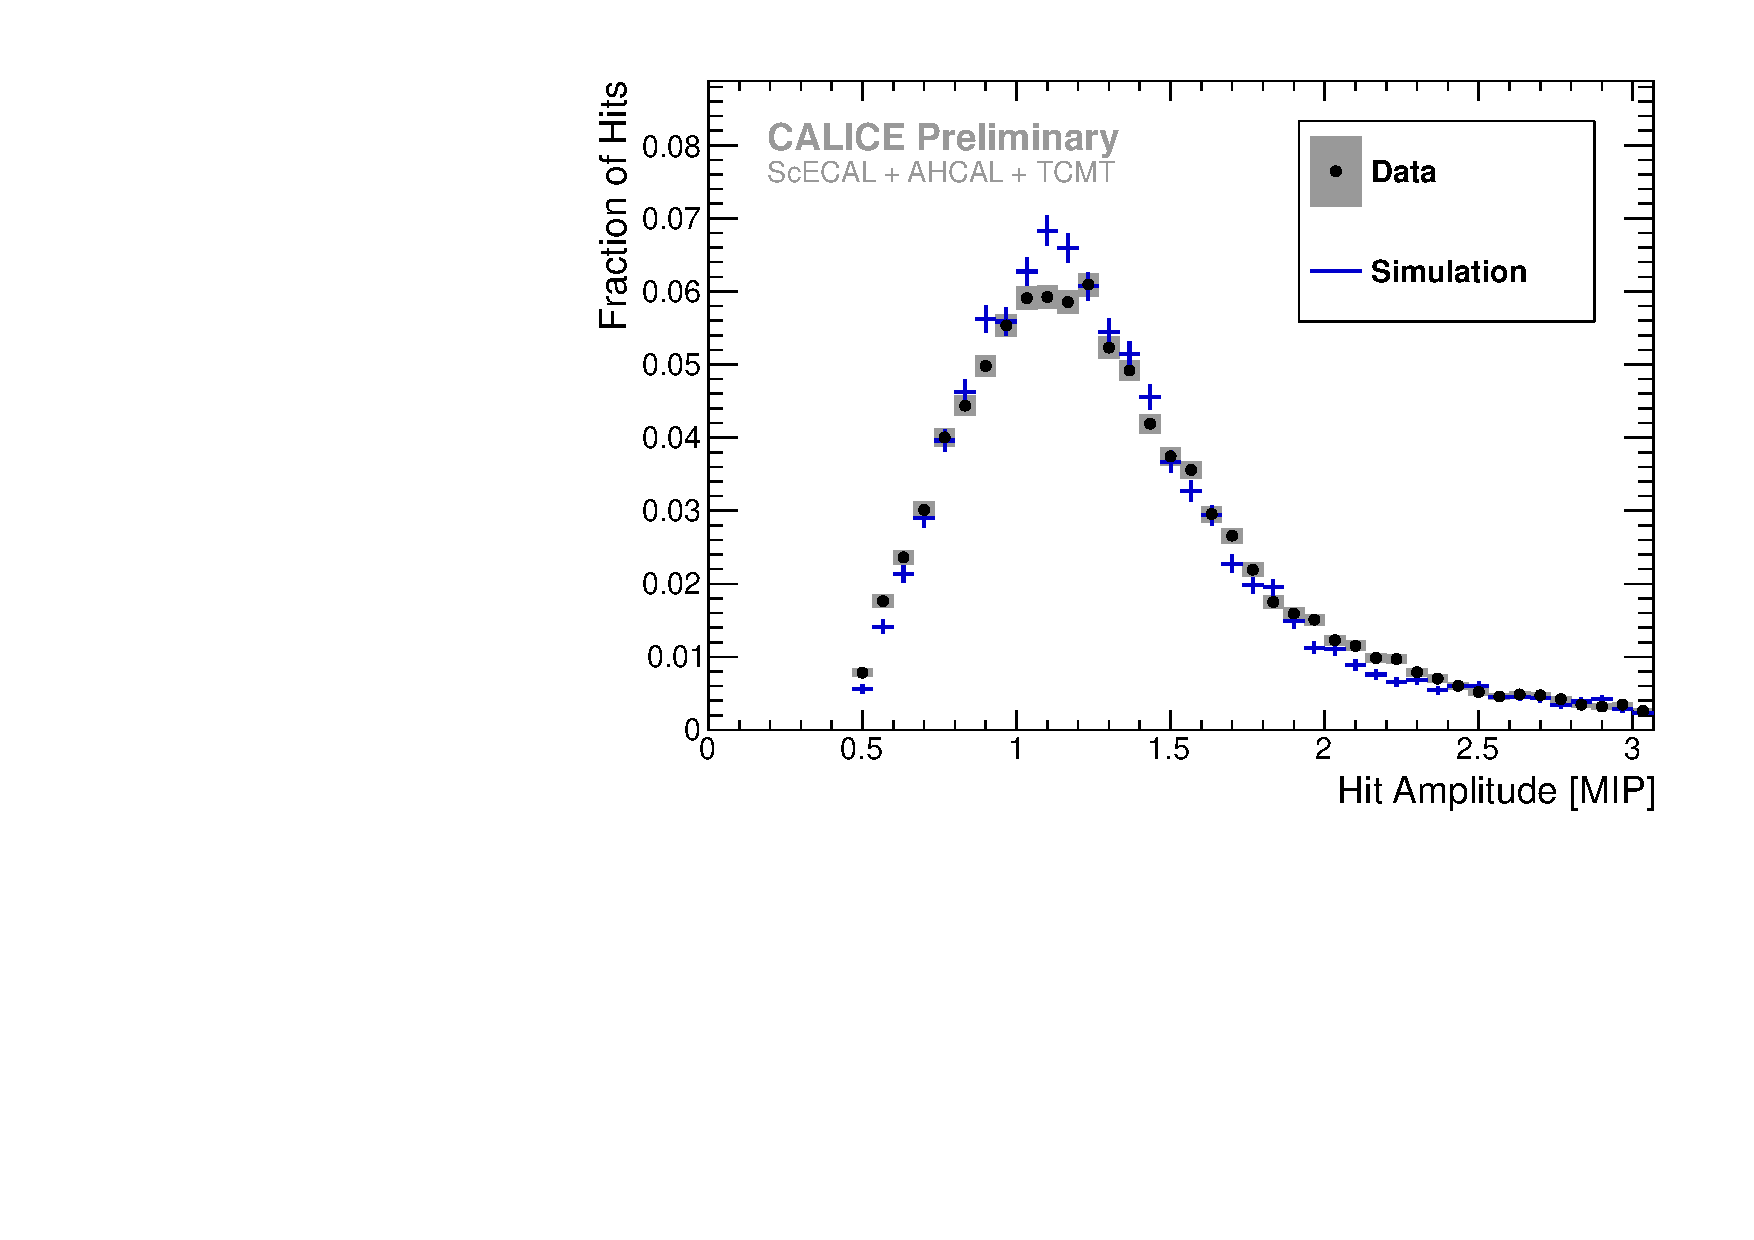
\includegraphics[width=0.50\textwidth]{fig/electron/mipspectrum_single_ecal_560474.pdf}}\hfill
	\subfigure[MIP Fit Distribution\label{fig:MIPmpv}] {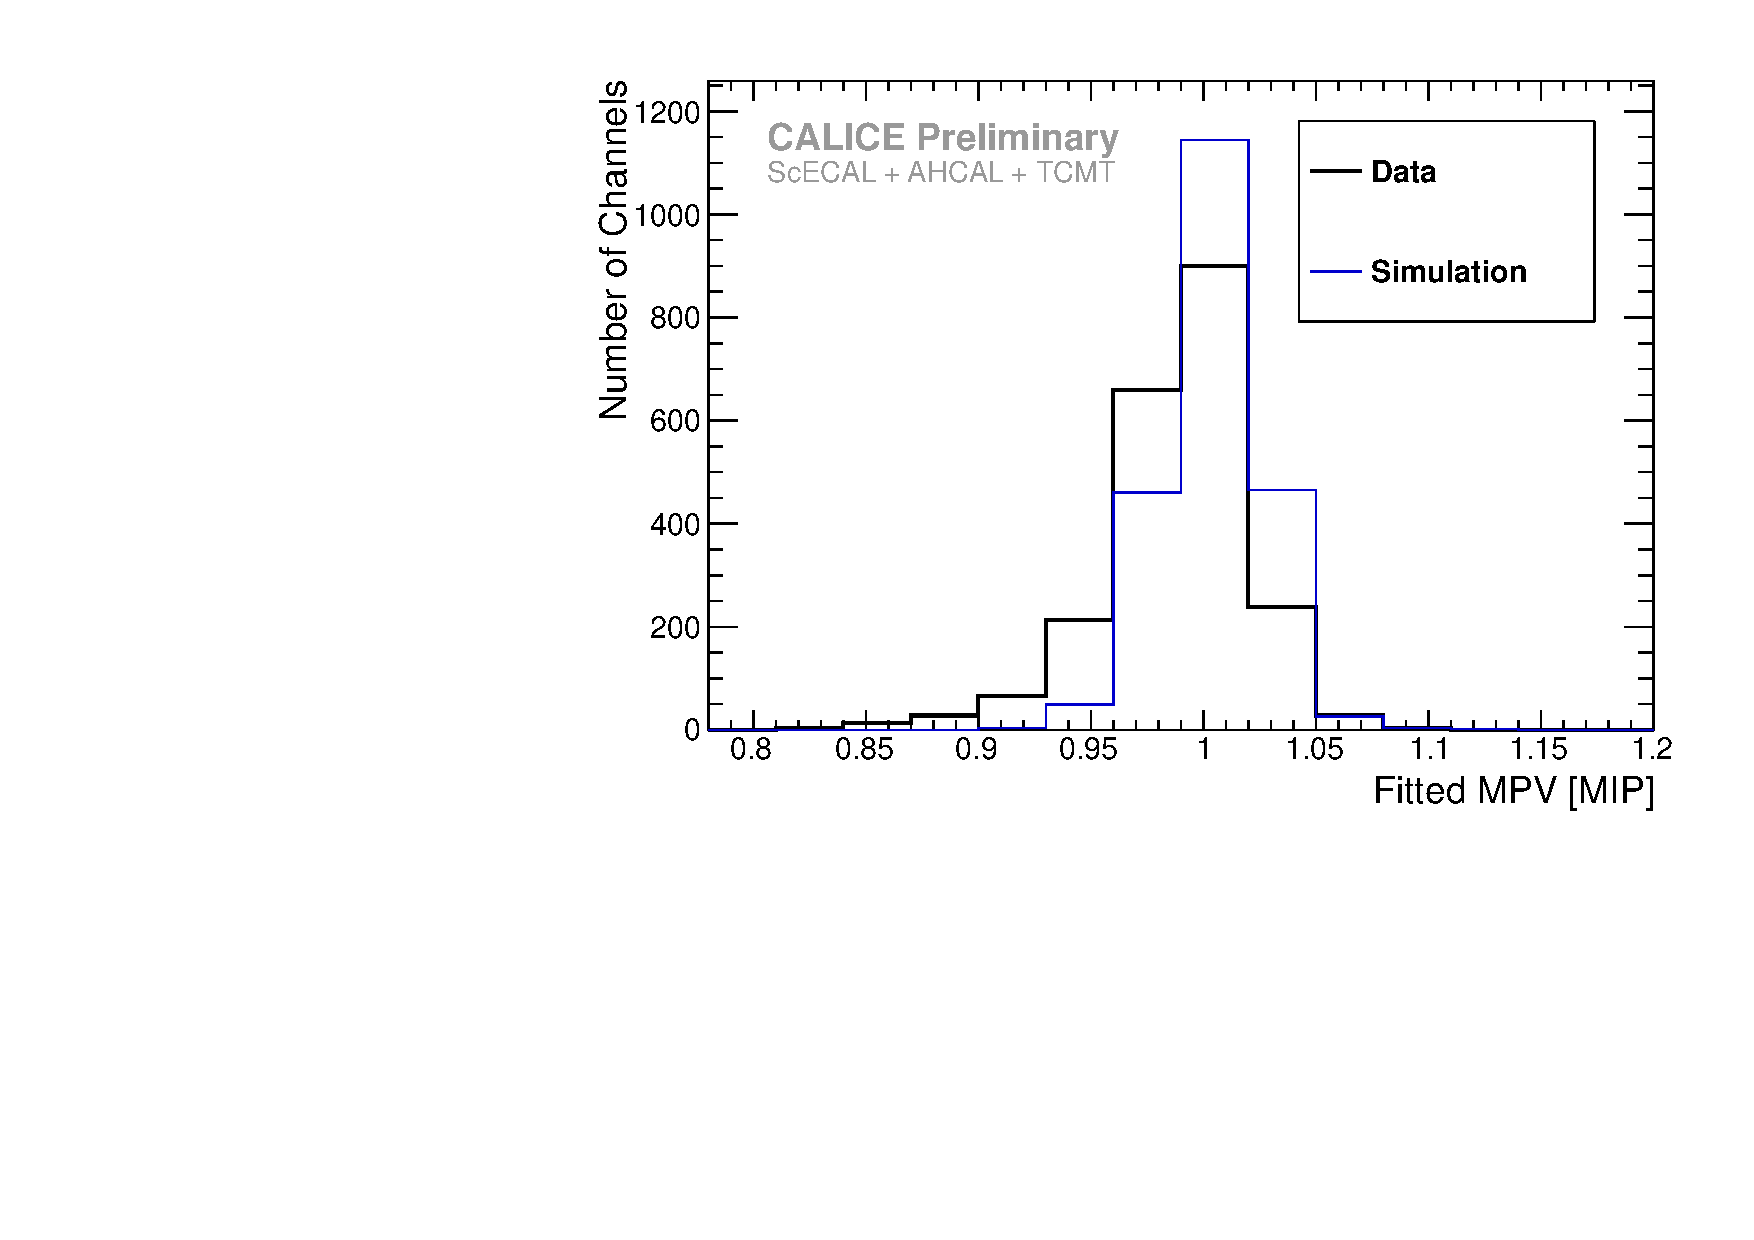
\includegraphics[width=0.50\textwidth]{fig/electron/fitmpv_ecal_560270.pdf}}
	
	\caption[]{Comparison of MIP-like particles in data and simulation. \\\textbf{(a)}: Hit energy spectrum of a single ScECAL cell in run 560474 (32\,GeV \piminus), normalised to the number of hits. \\\textbf{(b)}: Distribution of fitted most probable values of fits to the MIP spectra in single ScECAL cells from Run 560269 (32\,GeV \muminus). \\$\mu_\text{data}=0.99, \text{RMS}_\text{data}=0.040, \mu_\text{MC}=1.00, \text{RMS}_\text{MC}=0.022$.}
	\label{fig:MIP}
\end{figure}

To perform further comparisons on electron showers, a sample of single electron events is selected from the recorded data runs. A simple electron selection, based on the inversion of the pion selection described in \autoref{sec:pionselection}, incorporating the beamline Cherenkov counters and beam scintillators, is applied. As even electrons of the highest energy available from the beamline are expected to be fully contained in the ScECAL, additionally only events with low activity in the AHCAL are accepted to reject pions. A detailed list of cuts performed is given in \autoref{table:electronselection} in the Appendix. As shown in \autoref{fig:cutflow_electron} the selection yields a clean sample of single electron events. 

\begin{figure}[htbp]
\begin{center}
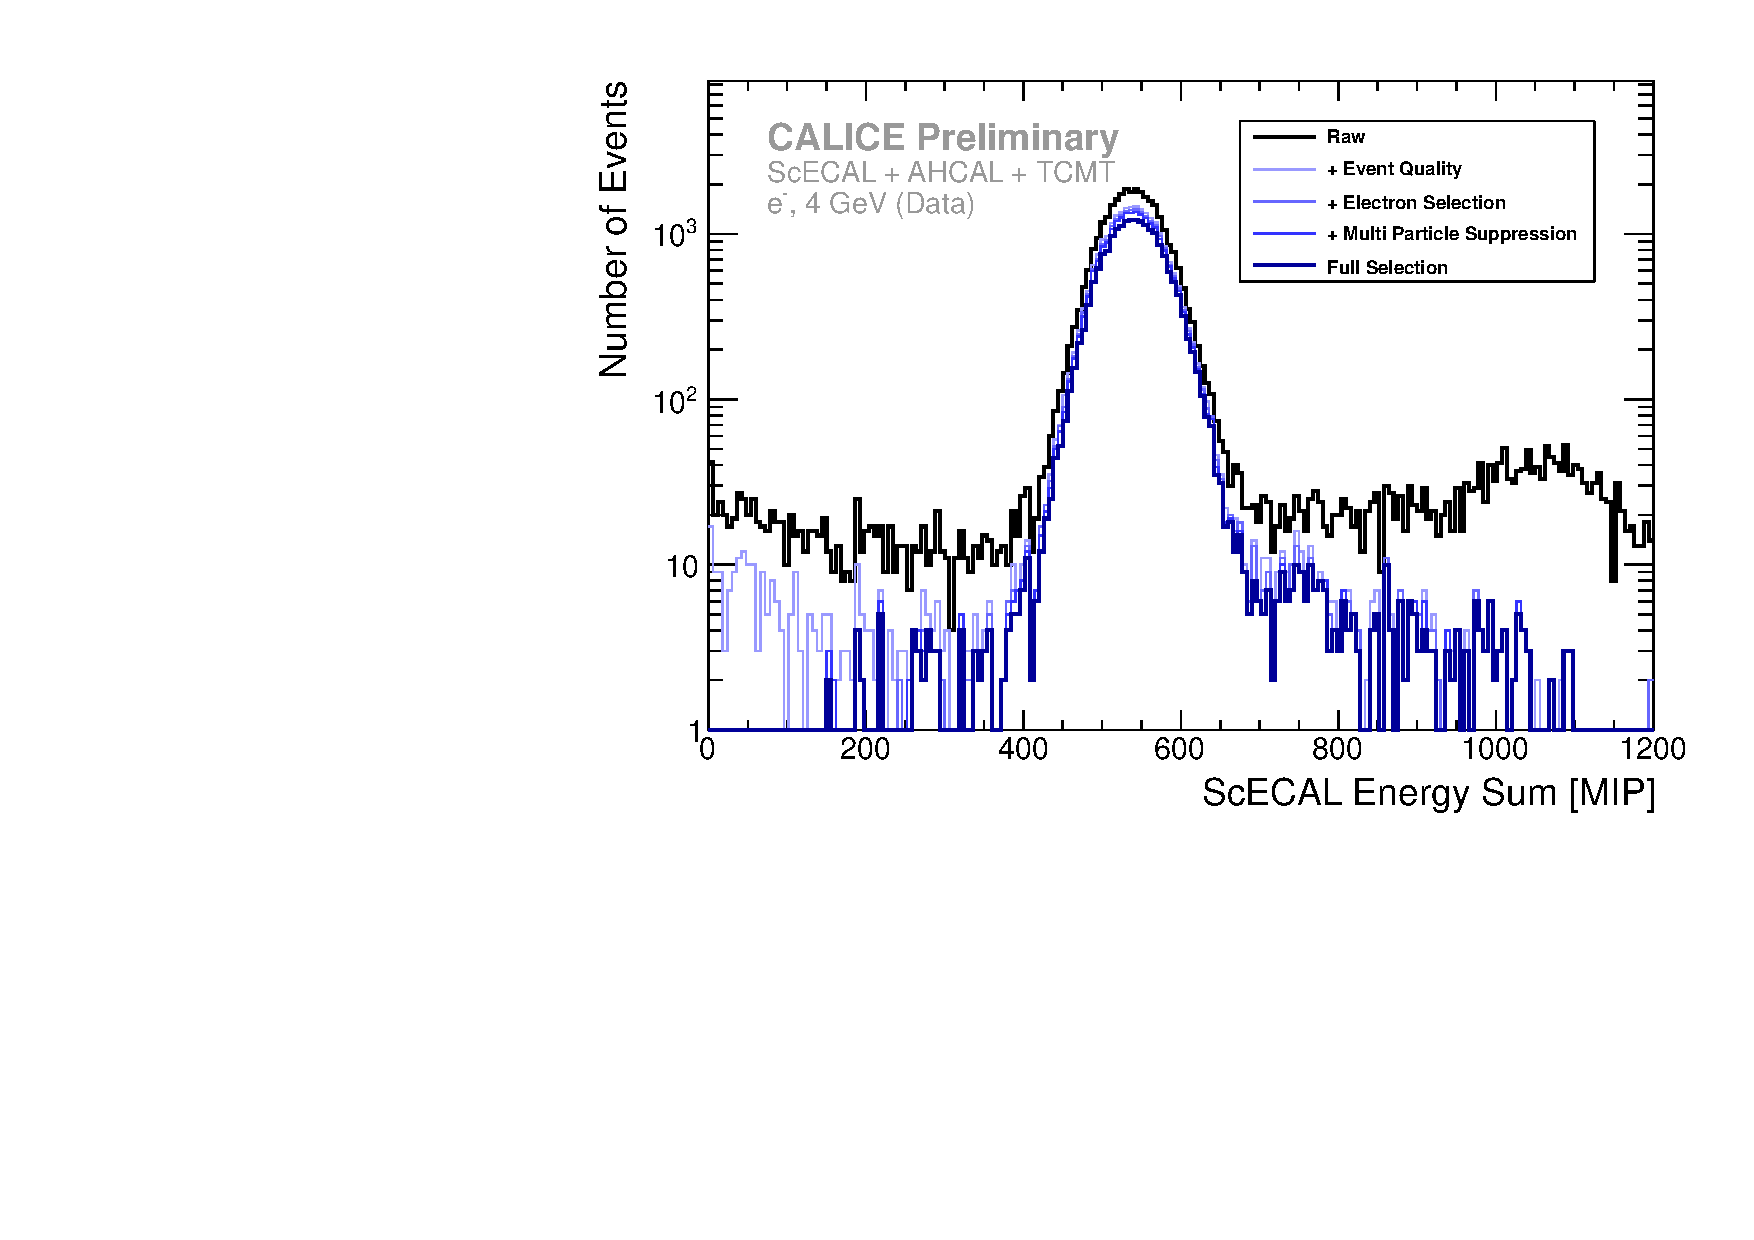
\includegraphics[width=0.8\textwidth]{fig/electron/ERec_cutFlow_560332_data.pdf}
\caption{Reconstructed energy spectrum of data run 560332 (4\,GeV \eminus) for different steps of the applied event selection.}
\label{fig:cutflow_electron}
\end{center}
\end{figure}

The comparison of hit energy distributions in Figure \ref{fig:electron_hitenergy} shows a significantly longer tail towards higher hit energies in simulated events than data. Assuming a perfect description of the physics of electron showers in the simulation, this could be either caused by a wrong or incomplete treatment of SiPM saturation effects or a wrong material description in the simulation model.

The unfolding of SiPM saturation in ScECAL data is performed by assuming the same number of effective pixels per sensor for all cells, using the mean of the number of effective pixels measured from a subset of ScECAL strips (as described in detail in \cite{CAN16b}). Re-reconstructing the dataset with this parameter reduced by 20\% ($\approx 2\sigma$ of the measured distribution) yields the spectra and profiles labelled as \emph{Data (Sat. Scale)} in the following. This leads to slightly longer tails in the hit energy distribution in data for all beam energies, although not enough to make data and simulation agree, as shown in \autoref{fig:electron_hitenergy}. However the specific behaviour observed in the type of SiPM used in the ScECAL (see \cite{CAN16b}) is not included into the desaturation calculation during reconstruction and is still under active investigation \cite{SiPMNLO}.

An incorrect description of the materials in the simulation model would lead to a discrepancy in observed shower profiles between data and simulation. The transverse shower profile, as the distribution of energy weighted distances to the reconstructed center-of-gravity of the shower, in \autoref{fig:electron_transverse} indeed shows a significantly narrower shower core in simulation compared to data for all beam energies, leading to higher energy deposition densities and thus potentially explaining the harder hit energy spectrum. The longitudinal profile in \autoref{fig:electron_longitudinal} is however well described, indicating that the amount of absorber material in $\nicefrac{X_0}{\text{Layer}}$ is well modelled in simulation. The only way to increase the effective \emph{Moli\`ere Radius} $r_M$ nearly without influencing $\nicefrac{X_0}{\text{Layer}}$ is increasing the thickness of air between individual ScECAL layers. Separate simulations with modified air gap between individual ScECAL layers (doubled from 1.24\,mm to 2.48\,mm) labelled \emph{MC (Airgap*2)} are shown in the figures below. The wider air gap slightly increases $r_M$ and reduces the tail in the hit energy spectrum, but not enough to make the simulation agree with data. A further increase of the air gap is entirely unphysical, as the doubled air gap already makes the modified ScECAL simulation model $30\cdot1.24\,\text{mm} \approx 3.7\,\text{cm}$ longer than the measured length of the ScECAL prototype. Possible effects from remaining pion contaminations are considered to be small, as the pion fraction should show a strong dependence on the beam energy, while the observed mismatch in the transverse shower profile is  We thus consider the possibility that the simulation model used in this study indeed produces slightly too narrow electromagnetic showers. Shifting the saturation scale in data reconstruction has a small influence on the measured transverse shower profile, but does not improve the agreement with simulations.

The studied effects produce shifts in the order of the observed discrepancies between data and simulation in the hit energy spectra while keeping the longitudinal profile compatible to data, but the description of the transverse shower profile does not improve in the same way. No final conclusion whether the discrepancies between data and simulation can be attributed to the shower simulation or the geometry modelling and SiPM saturation can be drawn.   
The datasets obtained with modified simulations and reconstruction parameters are thus used as estimates on the systematic uncertainties on shower simulation, geometry modelling and SiPM desaturation.

\begin{figure}[htbp]
	\subfigure[Hit Energy Distribution\label{fig:electron_hitenergy}] {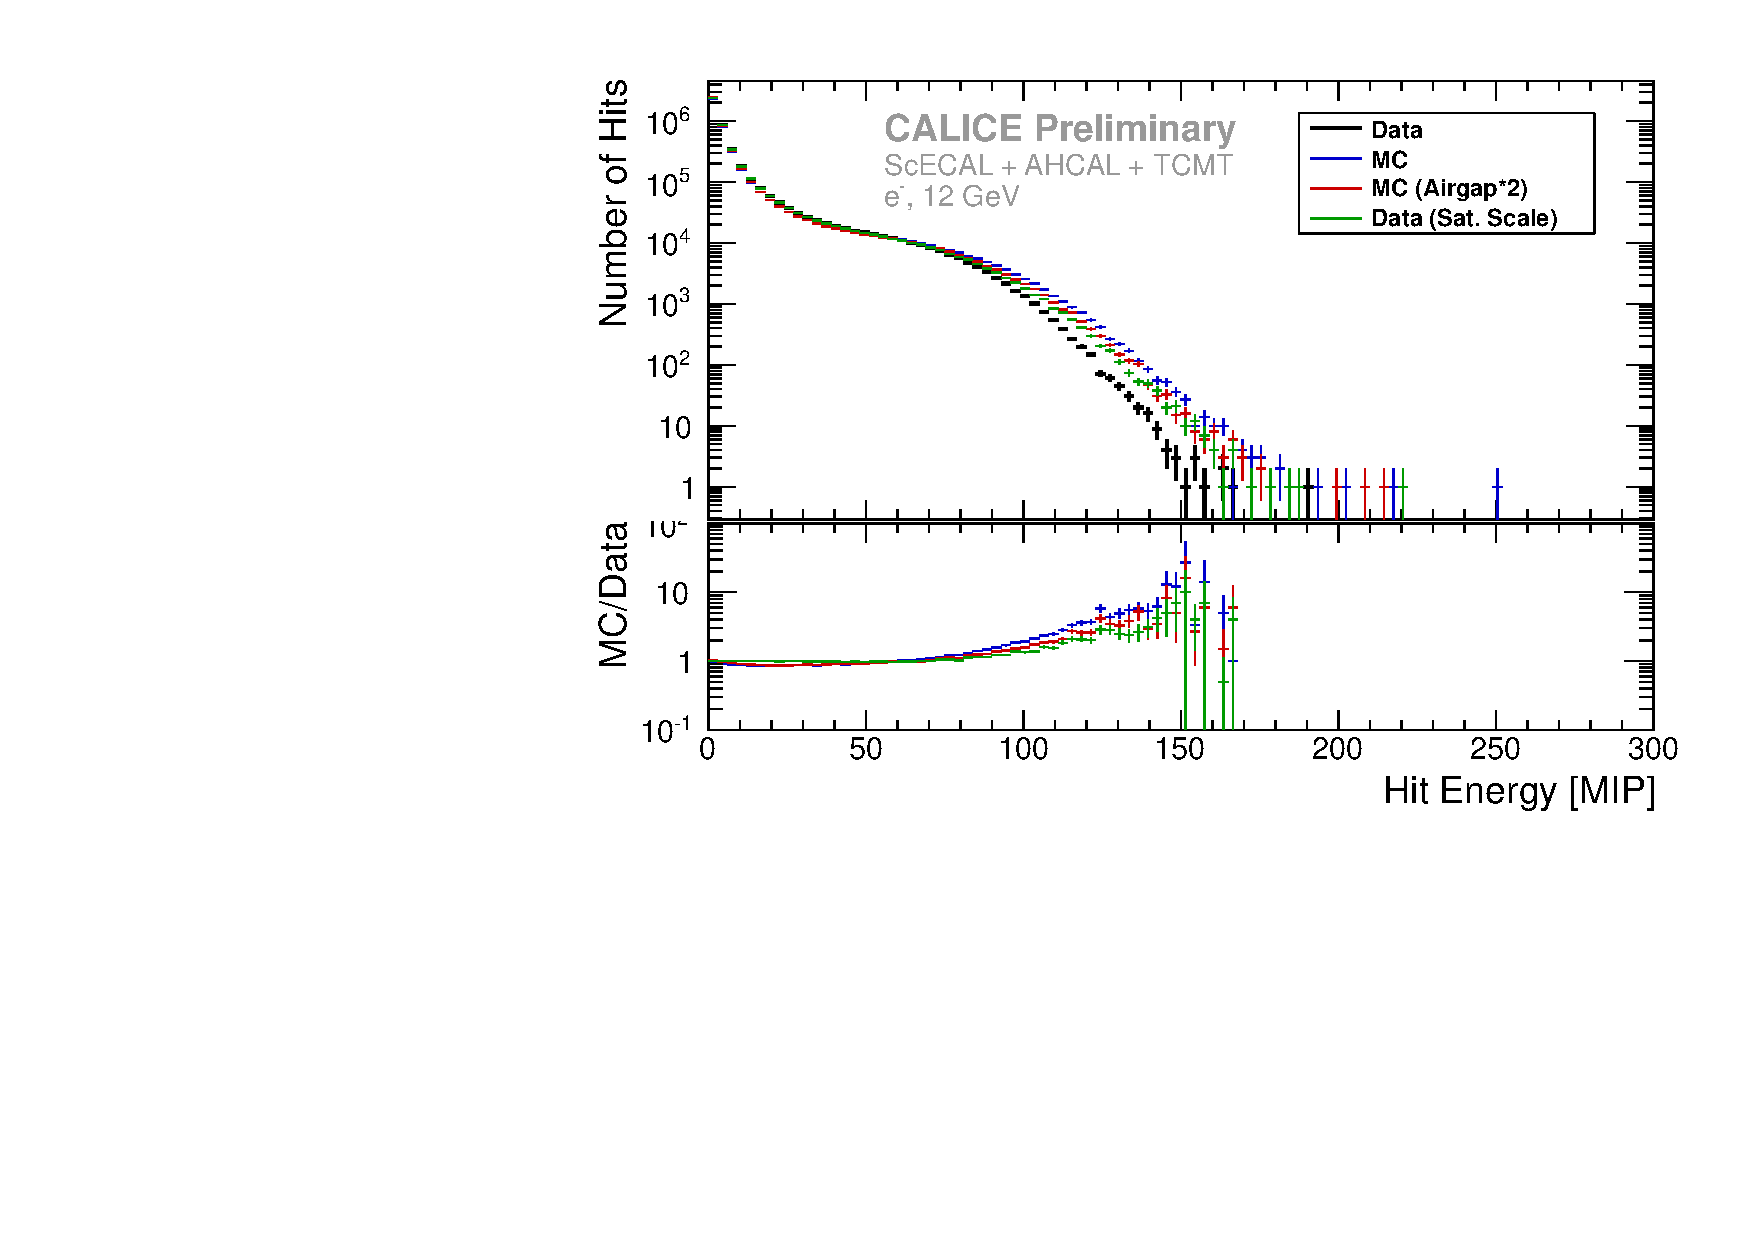
\includegraphics[width=0.50\textwidth]{fig/electron/out_hitEnergy_560294_12GeV.pdf}}\hfill
	\subfigure[Transverse Shower Profile\label{fig:electron_transverse}] {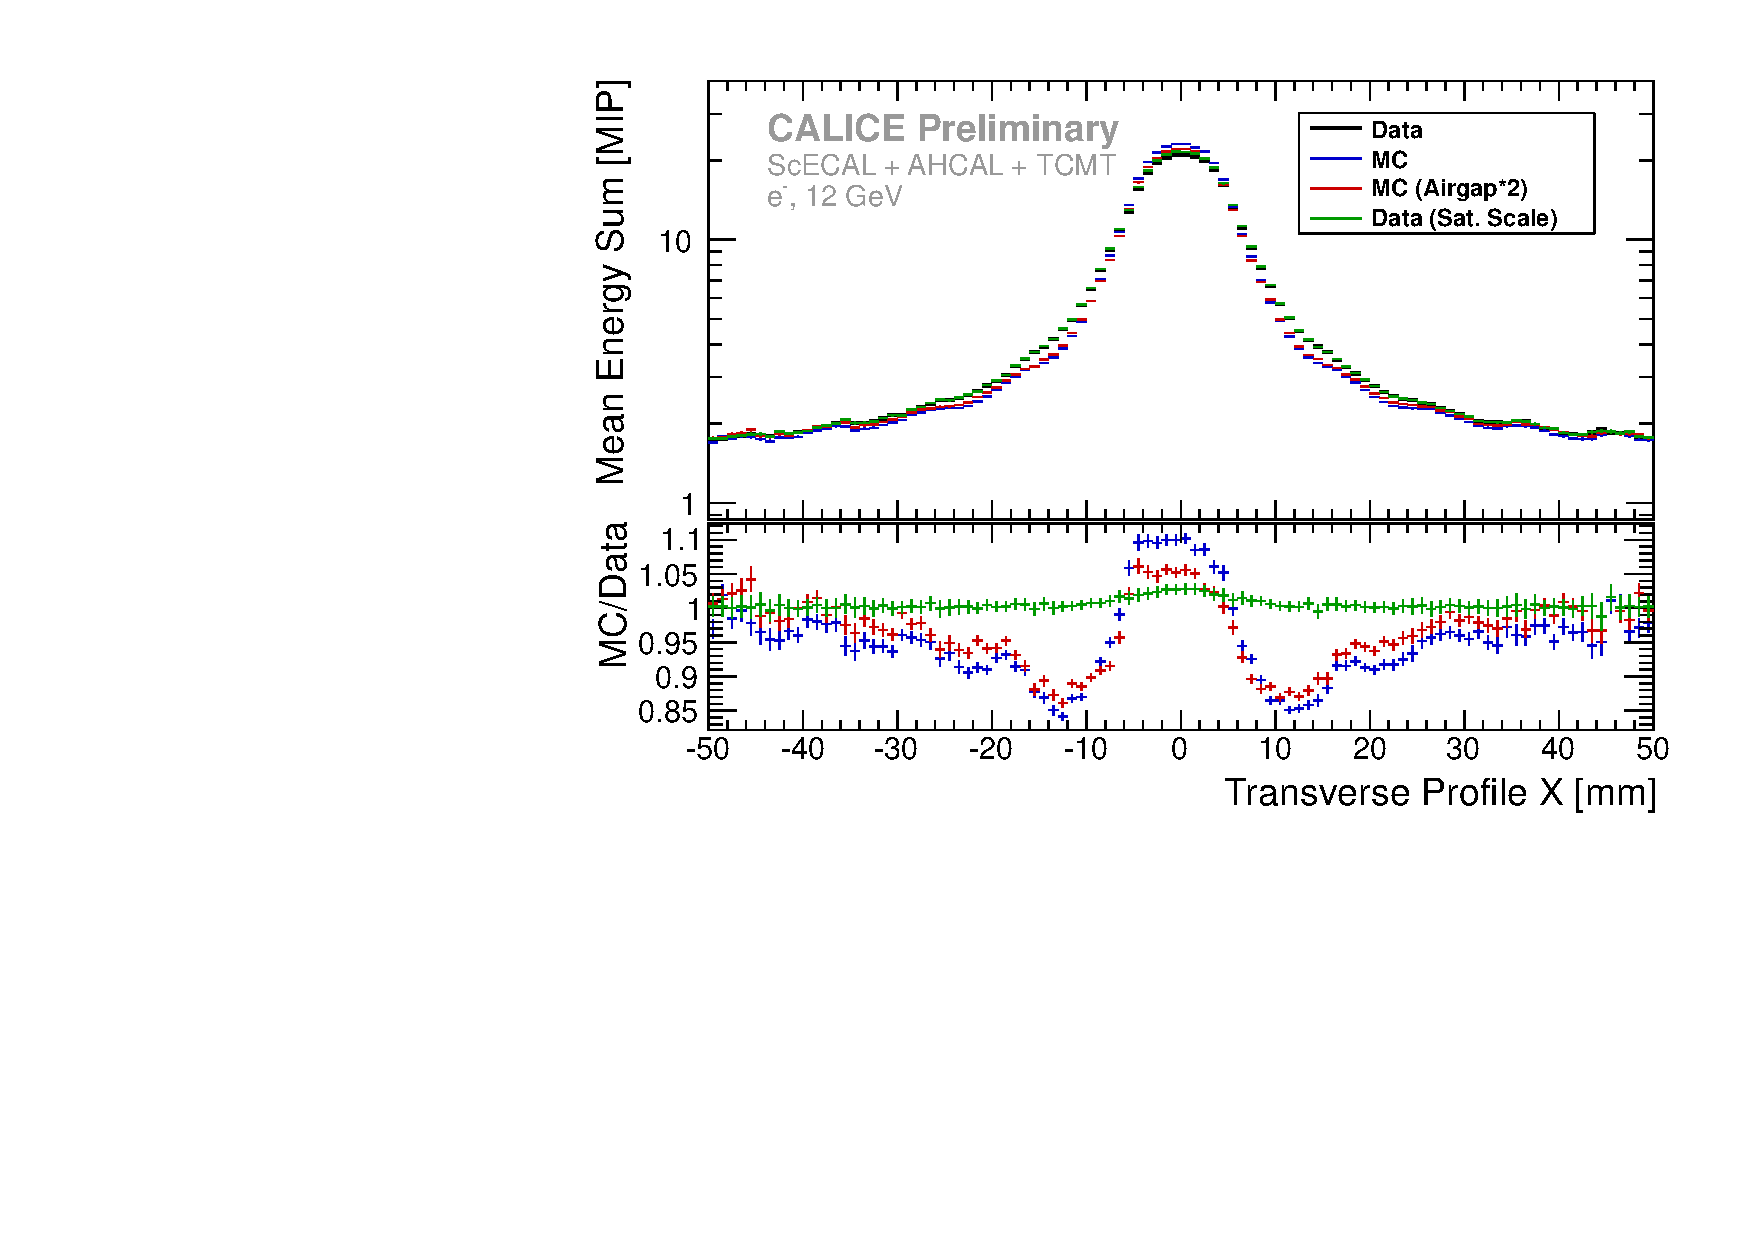
\includegraphics[width=0.50\textwidth]{fig/electron/out_profileRadial_560294_12GeV.pdf}}
	
	\caption{Electron shower hit energy distribution and transverse shower profile of run 560294 (12\,GeV \eminus) for data, simulation and possible systematic effects in simulation and reconstruction. \emph{MC (Airgap*2)} are simulated events obtained from a simulation model with doubled amount of air between ScECAL layers. \emph{Data (Sat. Scale)} is the same raw data set as \emph{Data}, but with the effective number of SiPM pixels used for saturation unfolding reduced by 20\% in reconstruction. }
	\label{fig:electron_profiles}
\end{figure}

The longitudinal profile of electron showers is generally well described by simulations in both shape and amplitude, see \autoref{fig:electron_longitudinal}. The remaining fluctuations from layer to layer can be accounted to channel-wise miscalibrations (which are not fully included in the simulation) in combination with most energy being deposited in few cells per layer. The systematic effects described in the previous paragraphs show very small influence within the existing fluctuations. Generally the measured response calibrated to the MIP scale in data and simulations agrees within a few \%, and the description of electromagnetic showers in simulation is satisfactory for the study of hadron showers.

\begin{figure}[htbp]
\begin{center}
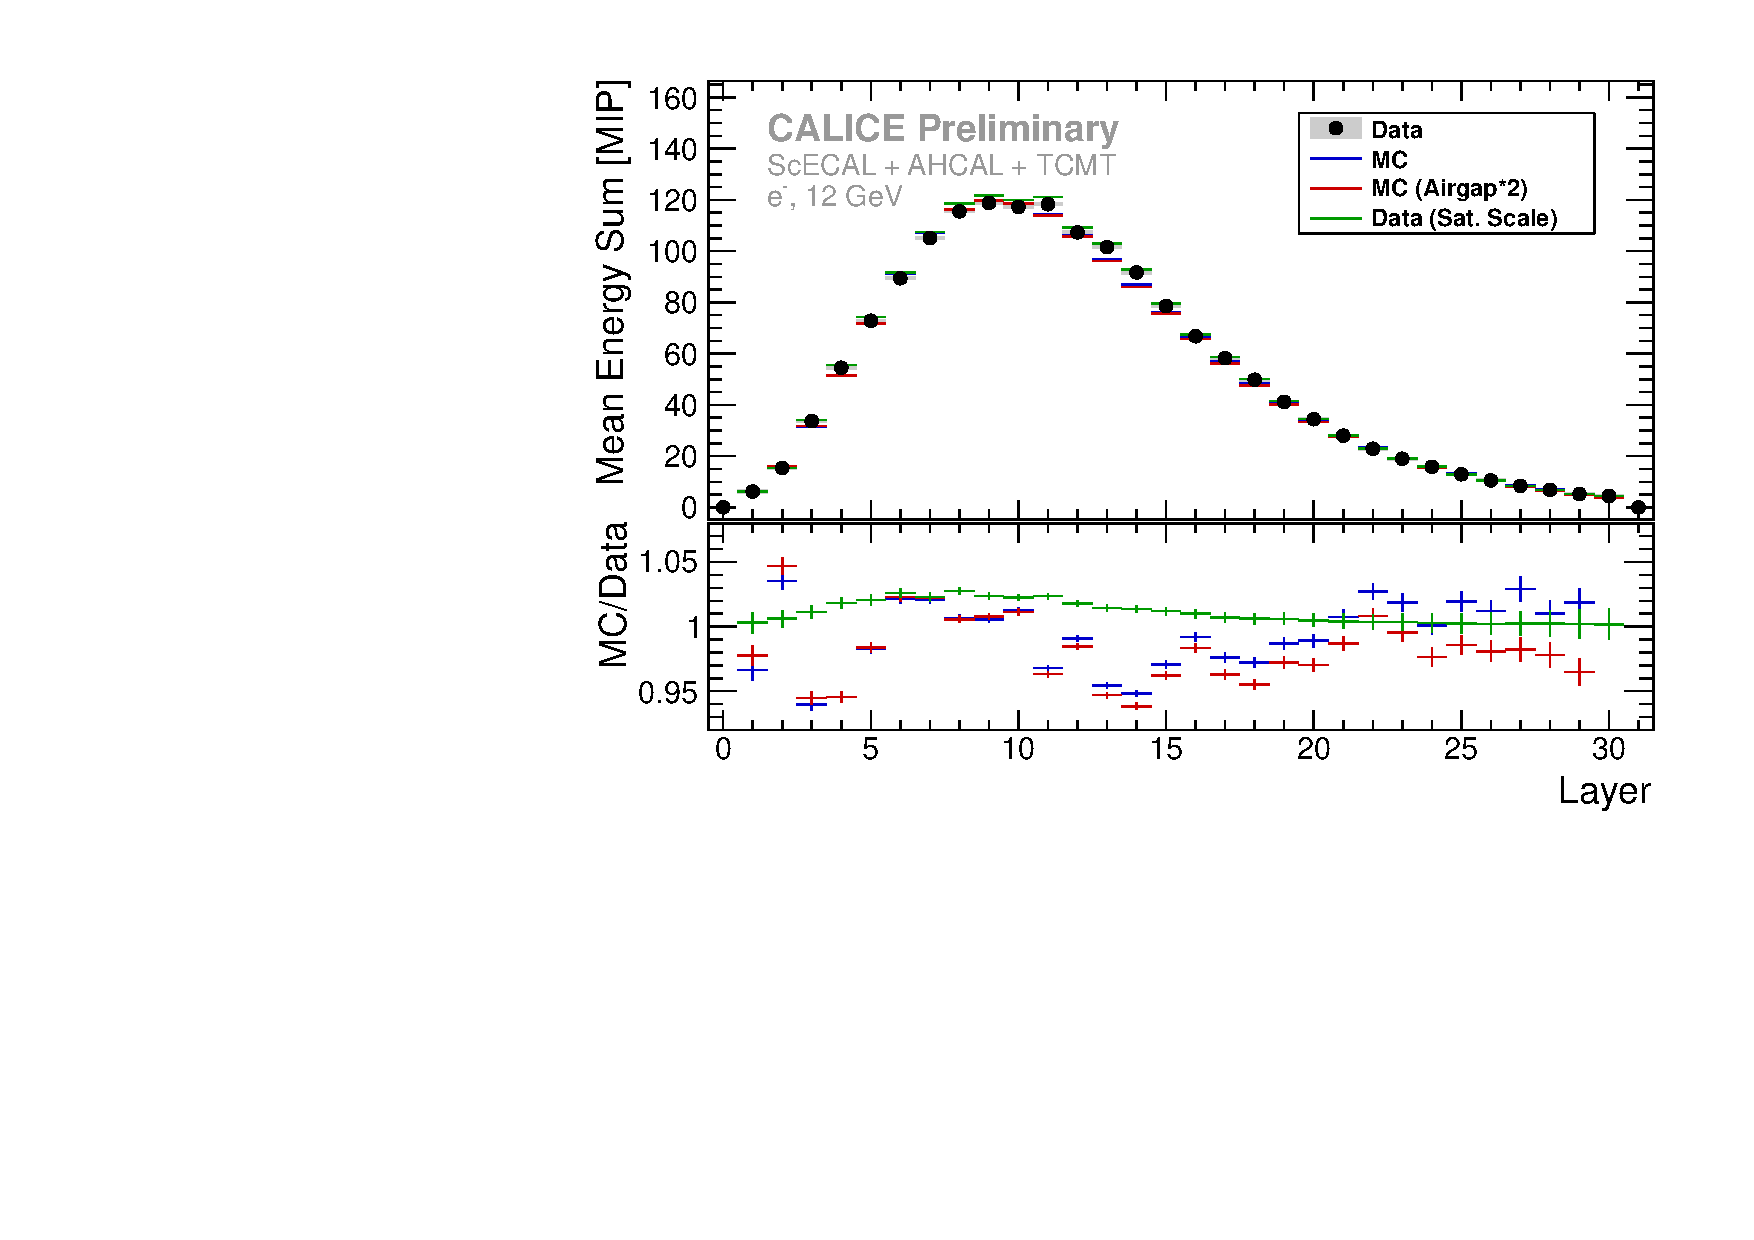
\includegraphics[width=0.8\textwidth]{fig/electron/out_profileLongitudinal_560294_12GeV.pdf}
\caption{Mean longitudinal shower profile of electron run 560294 (12\,GeV \eminus) for data, simulation and possible systematic effects in simulation and reconstruction.}
\label{fig:electron_longitudinal}
\end{center}
\end{figure}


\section{Run \& Event Selection}
During the FNAL testbeam period in 2009, \piminus-runs were taken with beam momenta ranging from 2\,GeV to 32\,GeV. 
The 2\,GeV energy point is omitted for containing a large admixture of electrons and multi-particle events as shown in \cite{Feege, FTBF}, a very wide beam profile due to multiple scattering in beam instrumentation and air downstream of the final selection magnet as well as inefficient and imprecise determination of the layer of first hard interaction, leading to an inefficient and impure selection of pions for further analysis.

The data and event numbers used for this analysis are listed in \autoref{table:pionruns}.

\begin{table}[htbp]
\begin{center}
\caption{Data runs used in this analysis, including number of events before and after selecting for single pions.}
\label{table:pionruns}
\begin{tabular}{r|r|r|r|r}
    \multicolumn{1}{c|}{Run} & \multicolumn{1}{c|}{Energy} & \multicolumn{1}{c|}{Events (raw)} & \multicolumn{1}{c|}{Events (sel.)} & \multicolumn{1}{c}{$\frac{\text{Events (sel.)}}{\text{Events (raw)}}$}\\\hline
   560506 & 4\,GeV & 202,943 & 45,518 & 22.4\% \\
560498 & 12\,GeV & 164,341 & 50,548 & 30.8\% \\
560496 & 15\,GeV & 225,112 & 69,058 & 30.7\% \\
560481 & 20\,GeV & 169,131 & 50,577 & 29.9\% \\
560474 & 32\,GeV & 215,992 & 60,596 & 28.1\% \\

\end{tabular}
\end{center}
\end{table}

\subsection{Pion Selection}\label{sec:pionselection}
As the MTest beamline at FTBF does not offer a direct selection of particle type apart from its polarity, the delivered particle beam is a mixture of mostly electrons, pions and muons in varying fractions depending on the beam energy. Especially for the lower range of beam energies there is also a large fraction of events with multiple particles hitting the calorimeters at the same time, see \cite{Feege,Guenter,FTBF}. The goal of the event selection described in the following is to efficiently select events containing a single, contained pion shower in the detector system. 

% \begin{figure}[htbp]
% 	\subfigure[Two pions traversing the ScECAL and showering in the AHCAL.] {\includegraphics[width=0.45\textwidth]{fig/pion/selection/eventdisplay_2pion.png}}\hfill
% 	\subfigure[Shower in the ScECAL extending into the AHCAL. Additional muon in the AHCAL extending through to the TCMT.] {\includegraphics[width=0.45\textwidth]{fig/pion/selection/eventdisplay_pion_muon.png}}
% 	
% 	\caption{Event displays with at least two particles in run 560498 (12\,GeV \piminus) before multi particle suppression cuts.}
% 	\label{fig:eventdisplays}
% \end{figure}

The first selection step evaluates readouts from the DAQ and external beam instrumentation, differential Cerenkov counters, the multi-particle counter and other trigger scintillators, as well as the exclusion of empty events (\emph{Event Quality}).

Then a \emph{Pion Selection} is performed to suppress electron and muon events in the sample. Single muons and punch-through pions are suppressed by rejecting events based on number of hits and center of gravity along the beam axis in the AHCAL as explained in \cite{Feege,Guenter}. Electrons are suppressed by requiring the reconstructed layer of first hadron interaction (FHI layer) to be $\geq5$, which also removes events that have started showering upstream of the calorimeters. The FHI layer reconstruction in the combined system is based on the \emph{AHCAL Primary Track Finder} algorithm \cite{MarinaFHI}, extended with optimised thresholds to also work in the ScECAL. The distribution of reconstructed FHI layers is very well described by all tested simulations models as shown in \autoref{fig:fhi_data_mc}.

\begin{figure}[htbp]
\begin{center}
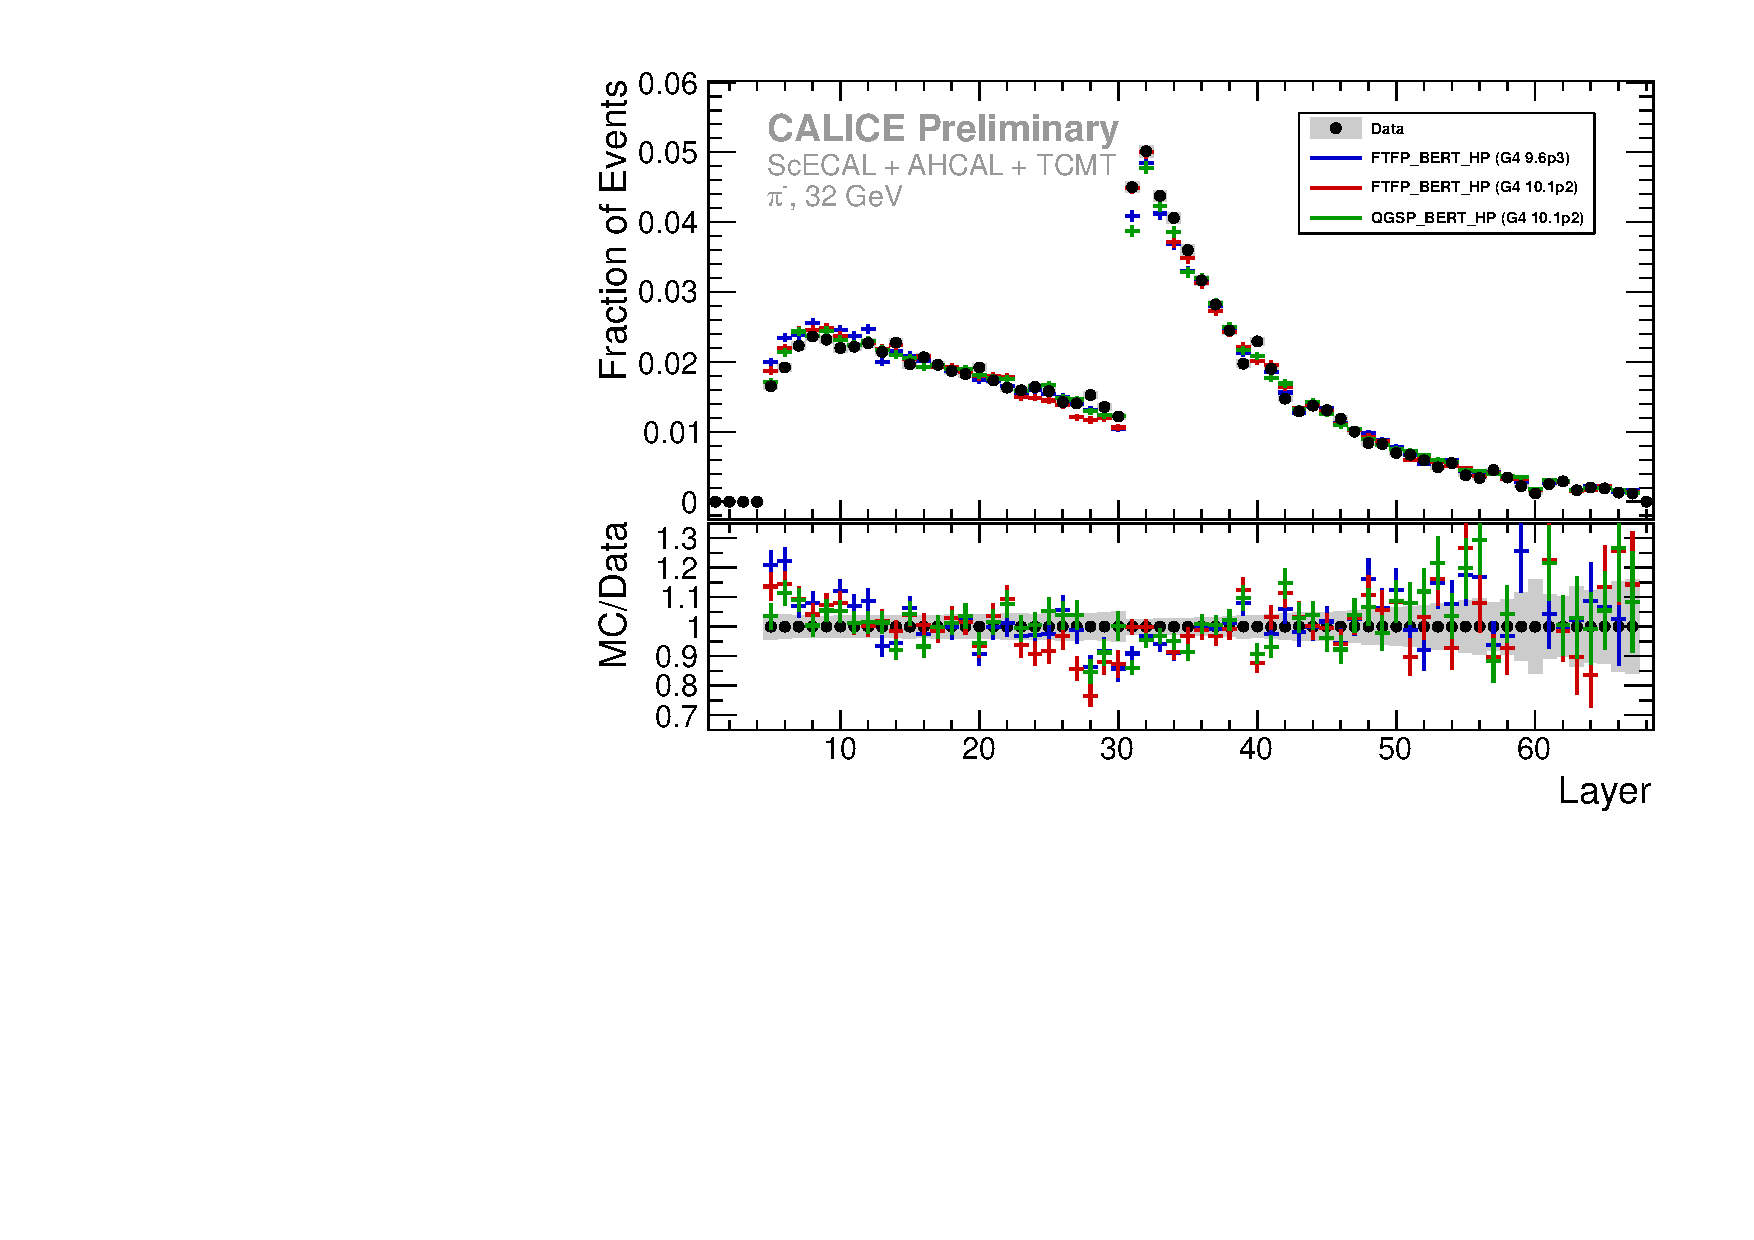
\includegraphics[width=0.8\textwidth]{fig/pion/selection/out_profileFHIlayer_560474.pdf}
\caption{Reconstructed FHI layer for 32\,GeV \piminus\ (Run 560474) in data and different simulation physics lists.}
\label{fig:fhi_data_mc}
\end{center}
\end{figure}

The suppression of events with multiple pion showers in the detector is achieved by reconstruction of the primary MIP-like track a pion is producing in the ScECAL before its first hard interaction. 
Only events with exactly one isolated primary track are selected. To suppress events with additional muons entering the AHCAL outside of the coverage of the ScECAL and multi particle counter, all events with tracks longer than five layers parallel to the beam axis in the outer parts of the AHCAL, reconstructed with the track segment finder algorithm described in \cite{TrackSegments}, are rejected (\emph{Multi particle suppression}).

Finally, to select for showers that are laterally and longitudinally contained, only events with the primary pion track around the center of the ScECAL and reconstructed FHI layer at the latest in the fifth AHCAL layer are accepted into the analysis (\emph{Containment}). The ratio of mean contribution to the reconstructed energy in ScECAL and AHCAL $r = \nicefrac{E_\text{rec}^\text{AHCAL}}{E_\text{rec}^\text{ScECAL}}$ varies from around unity (at 4\,GeV) to around three (at 32\,GeV). 

An example of the full step-by-step event selection in data and simulation is shown in \autoref{fig:cutflow}. The resulting reconstructed energy spectrum contains only a minor fraction around $10^{-2}$ remaining contamination in data, leading to only very small systematic uncertainties in the extraction of response and resolution. A detailed table of cuts performed is given in \autoref{table:pionselection} in the Appendix.

\begin{figure}[htbp]
	\subfigure[Data] {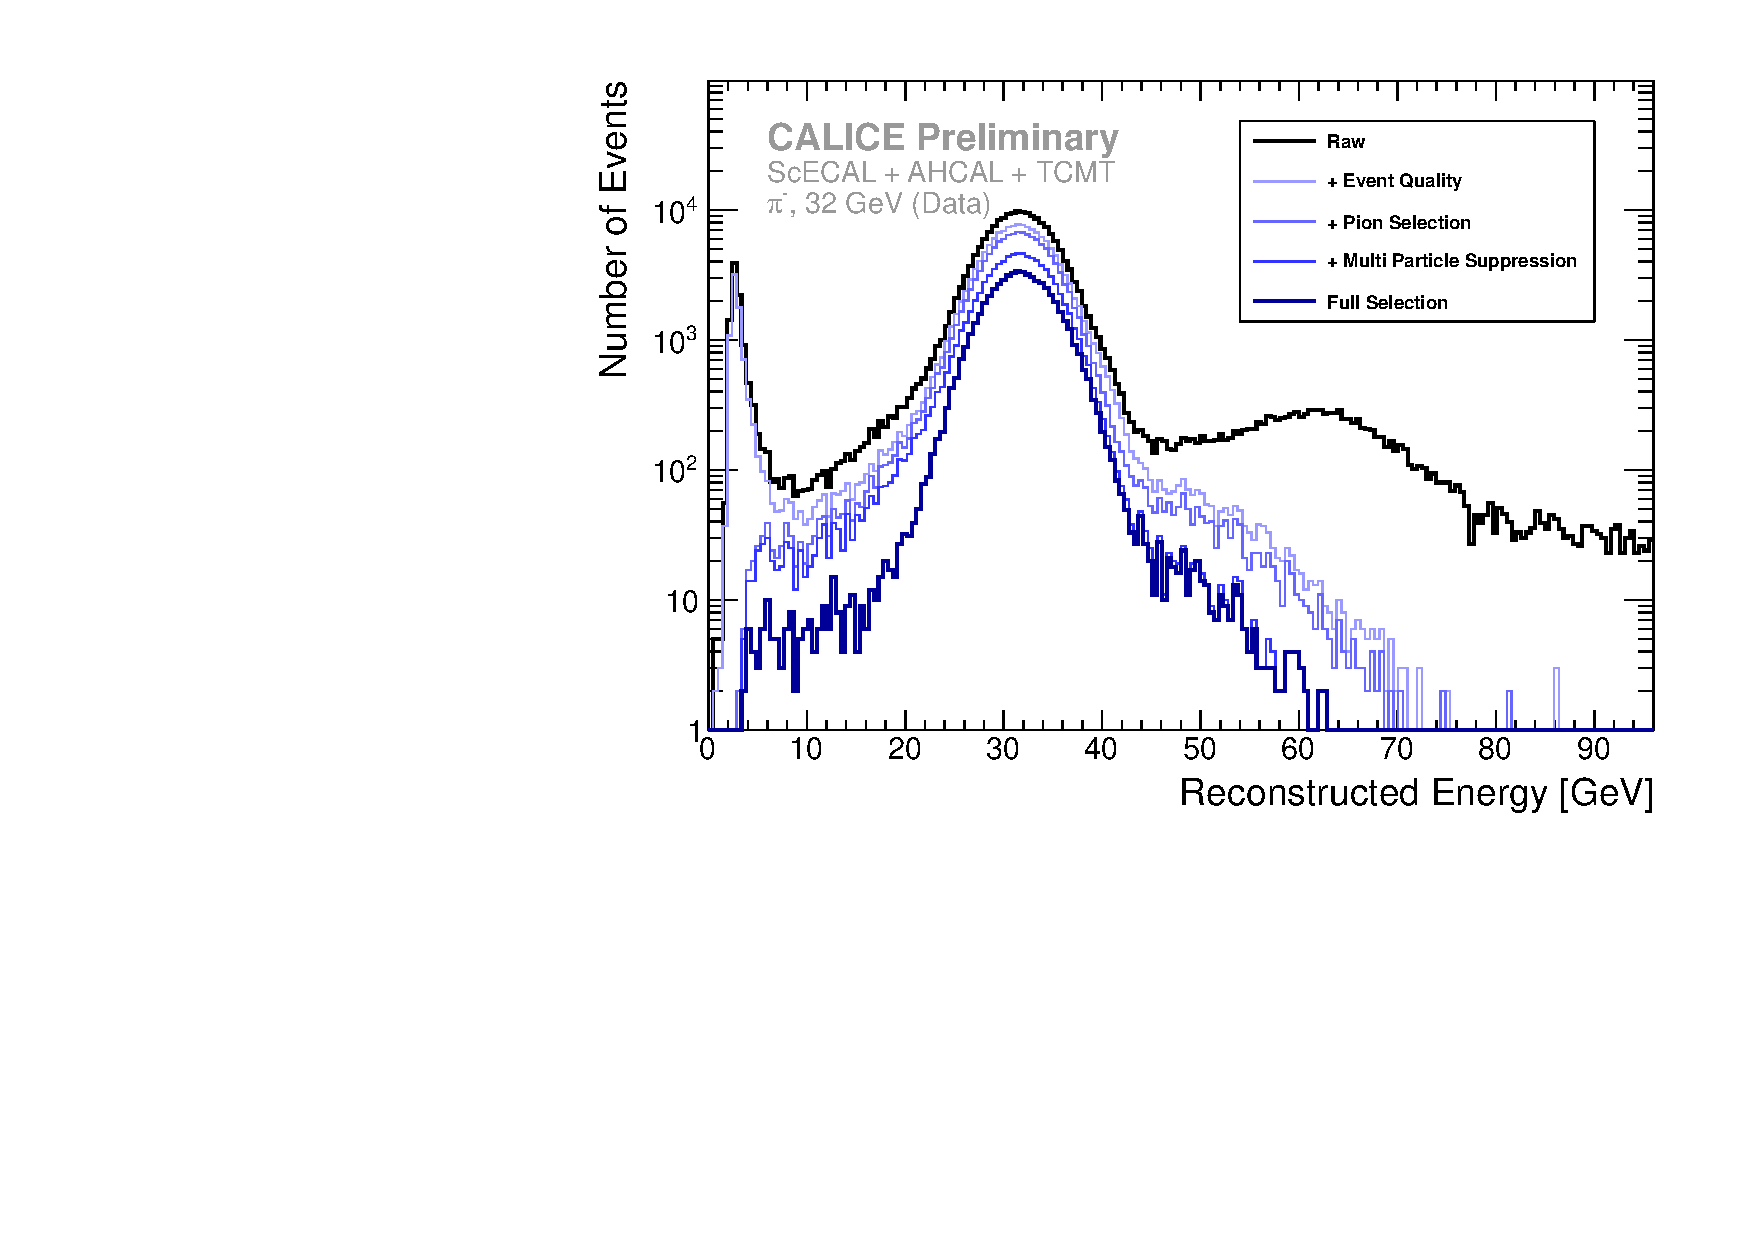
\includegraphics[width=0.5\textwidth]{fig/pion/selection/ERec_cutFlow_560474_data.pdf}}\hfill
	\subfigure[FTFP\_BERT\_HP (G4 10.1p2)] {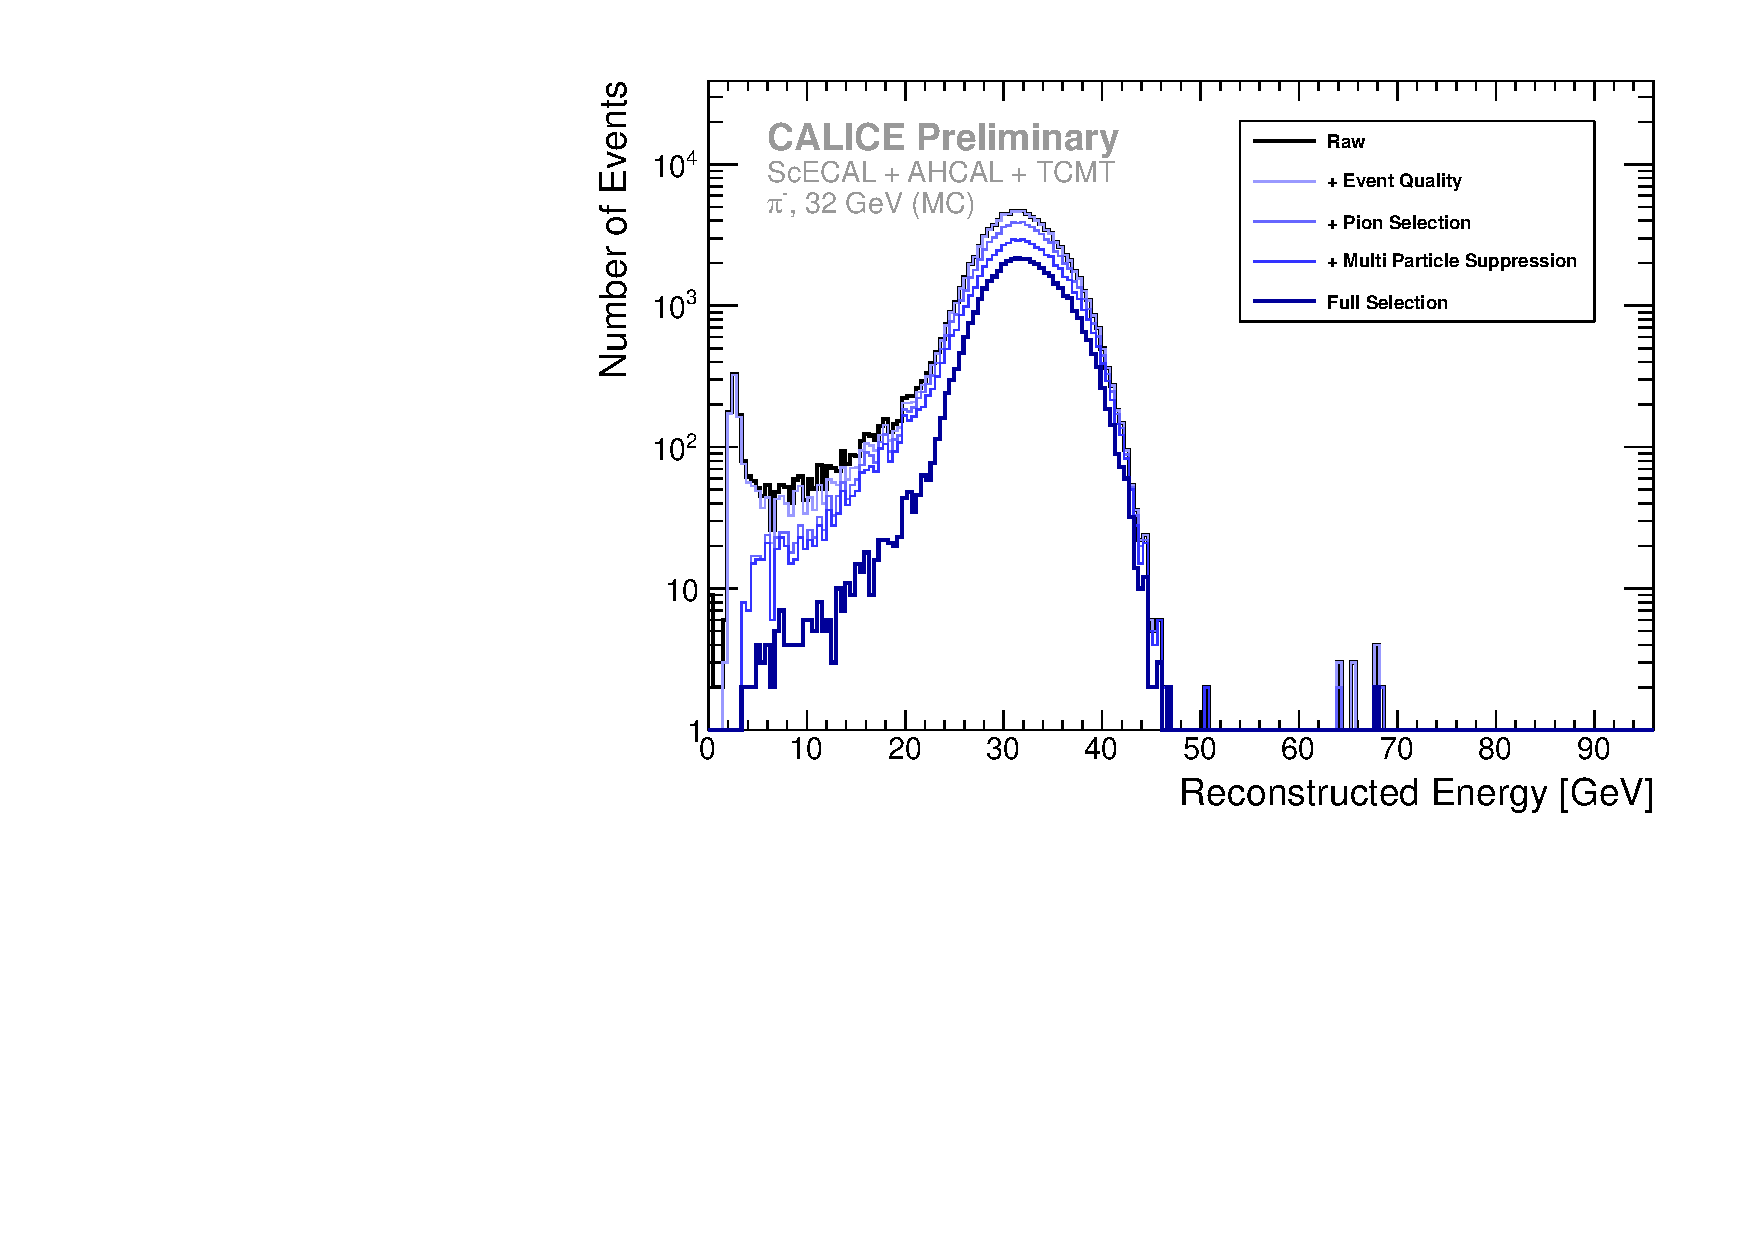
\includegraphics[width=0.5\textwidth]{fig/pion/selection/ERec_cutFlow_560474_FTFP.pdf}}
	
	\caption{Reconstructed energy spectrum of run 560474 (32\,GeV \piminus) in data and simulation for different steps of the applied event selection.}
	\label{fig:cutflow}
\end{figure}

Selection efficiencies and biases are studied from simulated event samples for different physics lists and particle types. \autoref{table:pionselectionMC} in the Appendix shows that 45--50\% of simulated pions pass the pion selection across all examined physics lists. Most of the excluded pion events are rejected by the FHI layer requirements for electron suppression and shower containment. From the selection requirements of FHI layer and isolated primary track an excellent electron suppression of $\gtrsim99.9$\% is achieved.

\autoref{table:pionselectionMC} also shows the fitted response and resolution (see \autoref{sec:energyrecoclassic}) to reconstructed energy spectra of simulated pion runs for all used beam energies and physics lists. This is done both for a minimal selection (\emph{FHI}) and the full pion selection (\emph{sel.}). The minimal selection contains the lower and upper cuts on FHI layer to roughly preserve sampling fractions and average containment between the selections. The bias on both response and resolution is $\lesssim1\%$ for all examined beam energies and physics lists.

\section{Pion Energy Reconstruction}\label{sec:energyreco}
This section describes how measured energy depositions in the different calorimeter prototypes are combined into a common reconstructed energy. This is achieved by applying a weight to each deposition according to the inverse sampling fraction of each calorimeter hit. In more complicated energy reconstruction schemes the reconstructed energy can depend on any number of measured event quantities and external parameters (\emph{weighting}). For any chosen energy reconstruction algorithm, external parameters can be optimised by minimising the sum of quadratic distances of the reconstructed event energy to the known beam energy, resembling a $\chi^2$ function:
\begin{equation}
\chi^2 = \sum_{events}\frac{\left( E_\text{rec}^\text{event}-E_\text{beam}^\text{event}\right )^2}{{\left(\frac{\sigma}{E}\right)}^2\cdot E_\text{beam}^\text{event}}
\end{equation}
In this formalism parameters can be estimated for multiple runs at multiple beam energies in one optimisation. 
In the energy range considered here, the variance of the reconstructed energy spectrum is expected to scale with the beam energy (according to the $\nicefrac{1}{\sqrt{E}}$ stochastic term resolution dependence). 
To normalise contributions to $\chi^2$ between different beam energies, each event is thus de-weighted by its known beam energy. The constant factor in the denominator is approximating the expected stochastic term of the calorimeter, using $\frac{\sigma}{E} = 55\%$ here, for energies given in GeV. This enables the correct parameter uncertainty estimation by the optimisation algorithm, but does not influence the estimated parameter values. In order not to bias the parameter estimation towards a specific beam energy, the same number of events are added to $\chi^2$ for each run. The first 40,000 selected events of each data run (20,000 in simulated runs) are used in the parameter optimisation. No significant difference in reconstructed energy resolution is observed whether the events used for parameter optimisation are excluded in the reconstruction or not for both energy reconstruction schemes discussed here.

\subsection{Standard Weighting}\label{sec:energyrecoclassic}
In an idealised sampling calorimeter, the reconstructed energy for an incoming particle is directly proportional to the measured depositions. For a calorimeter system consisting of several different sampling ratios, the reconstructed energy is the sum of all hit energies weighted by a constant factor for each calorimeter. As the sampling fraction within the ScECAL is constant and the AHCAL and first eight layers of the TCMT (depositions in the latter eight TCMT layers are disregarded in this analysis due to the limited beam energy range) have identical sampling fractions, the standard energy reconstruction only has two parameters $w_{\text{ECAL}}$ and $w_{\text{HCAL}}$:  
\begin{equation}
 E_\text{rec}^\text{classic}=w_{\text{ECAL}}\cdot E^\text{ScECAL}_\text{sum} + w_{\text{HCAL}}\cdot \left( E^\text{AHCAL}_\text{sum} + E^\text{TCMT}_\text{sum}\right) 
\end{equation}
The $\chi^2$-optimisation described above inherently assumes Gaussian distributions. The reconstructed energy spectra obtained from the used calorimeter setup can exhibit non-Gaussian features from fluctuations in the electromagnetic fraction of pion showers, leakage effects and sample impurities remaining in data. Thus the optimisation of weights is performed iteratively on the central 90\% of reconstructed energies. 

\autoref{fig:weights_classic} lists the weights both optimised for each beam energy on its own and all energies at once. The weight dependence on beam energy is flat, with the smallest beam energy point at 4\,GeV preferring slightly different weights. Weights optimised for all beam energies are close to the values obtained for single beam energies. All used physics lists produce very similar weights. Weights obtained from data have slightly ($\approx5\%$) higher values than weights obtained from simulations. This hints to a general overestimation of depositions in simulations, as can also be observed in the longitudinal shower profile (\autoref{fig:profile_long_full} in \autoref{sec:profiles}).

The reconstructed resolution and linearity only depend on the ratio of weights, which is very similar between data and simulations, as shown in \autoref{fig:weights_classic}. Using weights obtained from simulation to reconstruct data events (or vice versa) would thus not notably influence resolution, but only result in a shifted energy scale. 
\begin{figure}[htbp]
\begin{center}
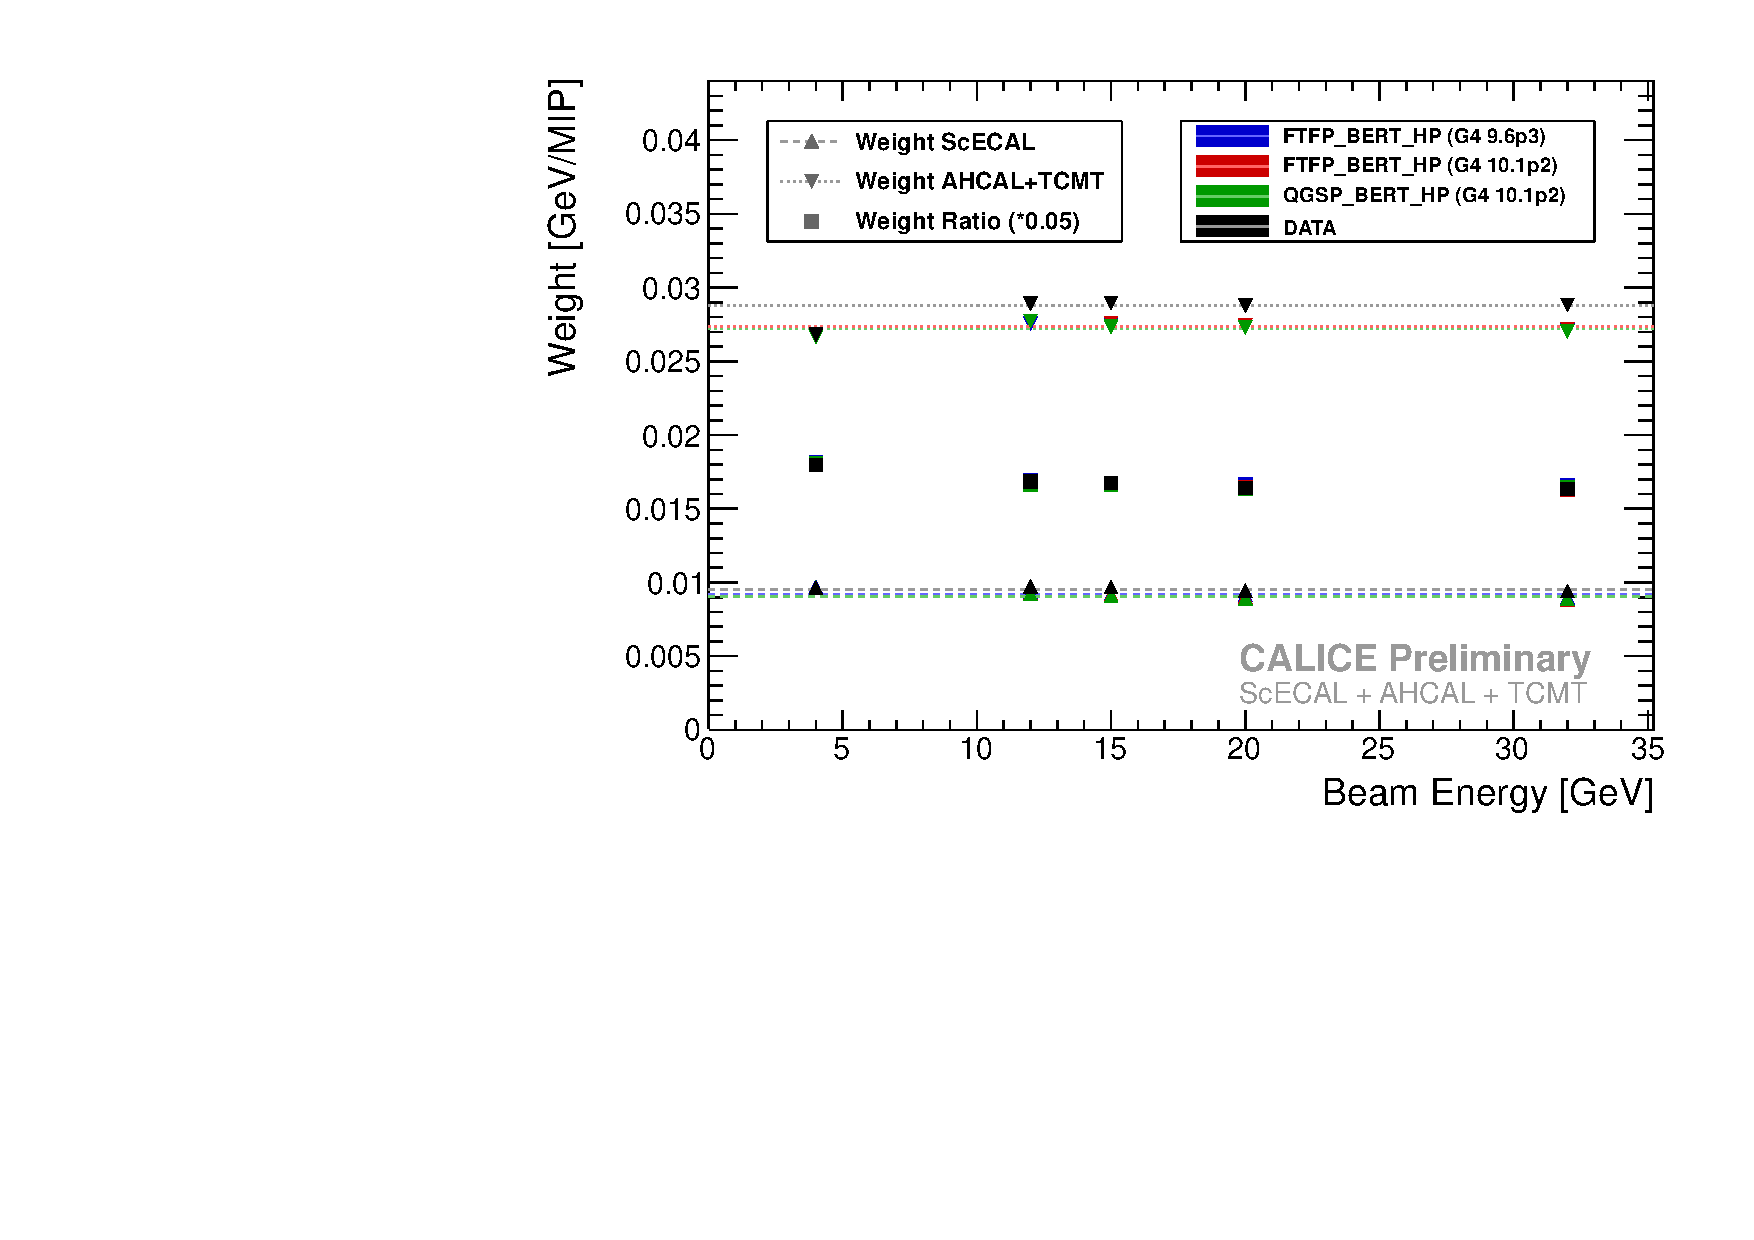
\includegraphics[width=0.8\textwidth,page=1]{fig/pion/classic/weightsClassic.pdf}
\caption{Standard energy reconstruction weights obtained from data and simulations. Markers indicate weights optimised for single beam energies, lines represent weights optimised for all available beam energy runs at once. All statistical uncertainties are smaller than the used markers.}
\label{fig:weights_classic}
\end{center}
\end{figure}
\subsection{Software Compensation}\label{sec:energyrecosc}
For most calorimeters, the measured response generated by a hadron shower is typically smaller than the response of an electromagnetic shower of the same initial particle energy ($\nicefrac{e}{\pi}>1$). Within hadron showers energy can be lost to \emph{invisible} processes like recoil, excitation and fragmentation of absorber nuclei and, depending on the active material, neutron emission. This leads to a lower response compared to purely electromagnetic showers. Hadron showers can also develop purely electromagnetic sub-showers from $\pi^0$/$\eta$ production in inelastic interactions and subsequent decay to two photons, yielding the full electromagnetic response for the two photons. 

Both the loss of measurable energy to \emph{invisible} mechanisms and the creation of $\pi^0$/$\eta$ are statistical processes and thus subject to significant fluctuations from event to event, leading to a large fluctuation in measured depositions and thus decreased energy resolution. Furthermore the number of generated $\pi^0$/$\eta$ particles depends on the number of inelastic interactions within a hadron shower and thus scales with beam energy, impairing the linearity of the calorimeter response. If it is possible to identify electromagnetic sub-shower contributions within hadron showers, reweighting them down to the purely hadronic deposition scale should lead to an improvement in resolution and linearity of the reconstructed energy.

With the materials used in this setup, the length scales of hadron showers and electromagnetic showers are notably different ($\nicefrac{X_0}{\text{layer}}\gg\nicefrac{\lambda_{\pi}}{\text{layer}}$ in both ScECAL and AHCAL). In combination with the high readout granularity of around the feature size of electromagnetic showers, this enables the differentiation between electromagnetic and hadronic shower components by deposited energy density. Each measured cell deposition is thus weighted as a function $w(\rho, E_\text{est.})$ of the local deposition density $\rho$ and an estimate of the full shower energy $E_\text{est.}$. 

Instead of fully parametrising $w(\rho, E_\text{est.})$, the dependence in $\rho$ is divided into fixed bins, while the dependence on $E_\text{est.}$ is parametrised over the used energy range for each such bin in this note. This scheme differs from the \emph{local software compensation} implementation in \cite{SCPaper}, which is iteratively parametrising $w$ in both $\rho$ and $E_\text{est.}$, by not enforcing any functional dependence on $\rho$, as $\rho$ is only ever evaluated in the chosen bins of deposition density. The scheme presented here leads to more free parameters and thus more degrees of freedom while improving the stability of the optimisation. 

Instead of using the deposition density as the hit amplitude divided by the cell size, the hit energy for each hit is used directly, disregarding the differently sized tiles in the AHCAL, slightly improving the performance of the full algorithm. This analysis uses eight hit energy bins. The obtained resolutions do not critically depend on the number of bins or exact bin boundaries. For the two lowest energy bins in the ScECAL and AHCAL, instead of summing up hit energies, only the number of hits falling into these bins are counted to suppress Landau fluctuations from low particle multiplicity hits (similar to the SDHCAL reconstruction \cite{SDHCAL}), slightly improving the resolution of the algorithm. All TCMT depositions are treated as falling into the same hit energy bin, effectively parametrising the relative TCMT weight as a function of the beam energy only.

The lowest hit energy bin has significant contributions from the primary track before the first hard interaction, which show nearly no dependence on beam energy. To exclude biasing of the parameter optimisation towards weighting up the primary track hits to the full beam energy, hits on the primary track are excluded from the software compensation weighting. All hits on the axis of the reconstructed isolated primary track (as described in \autoref{sec:pionselection}) from the first ScECAL layer up to two layers before the reconstructed FHI layer are included into the energy reconstruction without hit energy or shower energy dependent weighting. To exclude Landau fluctuations, only the number of such hits is used and multiplied by the mean energy deposition of a MIP-like particle in a single cell of the given calorimeter section.

An example of the distribution of hits into hit energy bins is given in \autoref{fig:hitEnergySCbinsData}. It is apparent that in the lowest hit energy bin in the ScECAL around one quarter of all contributions would come from the primary track if not identified and excluded. The contribution of primary track hits to the AHCAL hit energy spectrum is small, as around 70\% of selected events start showering in the ScECAL (see \autoref{fig:fhi_data_mc}).

\begin{figure}[htbp]
	\subfigure[ScECAL] {\includegraphics[width=0.5\textwidth,page=3]{fig/pion/SC/hitEnergyBins_DATA.pdf}}\hfill
	\subfigure[AHCAL] {\includegraphics[width=0.5\textwidth,page=8]{fig/pion/SC/hitEnergyBins_DATA.pdf}}
	
	\caption{Hit energy spectra of data run 560496 (15\,GeV \piminus), colours assigned to track hits and by software compensation bin.}
	\label{fig:hitEnergySCbinsData}
\end{figure}

%The full formula to reconstruct the energy in the combined system, with the sampling weights $w$, the bin weights for the $i$th bin $\alpha_i, \beta_i$ as well as the TCMT weight $\gamma$ are parametrised as a second order Chebyshev polynomial as a function of the estimated particle energy $E_\text{est.}$, the sum (or count) of energy depositions in the $i$th bin $E_i$ and the energy depositions on the primary track $E_\text{track}$, is:
In this analysis, the bin weights for the $i$th hit energy bin $\alpha_i, \beta_i$ as well as the TCMT weight $\gamma$ are parametrised as a second order Chebyshev polynomial as a function of the estimated particle energy $E_\text{est.}$.
The full formula to reconstruct the energy in the combined system, with the sampling weights $w$, the software compensation weights $\alpha_i, \beta_i$, $\gamma$, the sum (or count) of energy depositions in the $i$th hit enegy bin $E_i$ and the energy depositions on the primary track $E_\text{track}$, is:

\begin{multline}
  E_\text{rec}^\text{SC}=w_{\text{ECAL}}\cdot\left( \sum_{i}^{\text{bins}}\alpha_i\left(E_\text{est.}\right)\cdot E^\text{ECAL}_i+E^\text{ECAL}_\text{track}\right) \\ + w_{\text{HCAL}} \cdot\left( \sum_{i}^{\text{bins}}\beta_i\left(E_\text{est.}\right)\cdot E^\text{HCAL}_i+E^\text{HCAL}_\text{track} + \gamma\left(E_\text{est.}\right)\cdot E^\text{TCMT}_\text{sum}\right)
\end{multline}

The software compensation reconstruction is defined by 51 (8 bins in the ScECAL $\times$ 3 parameters per bin, $8\times3$ parameters for the AHCAL and $3$ parameters for the TCMT) parameters in total. In the optimisation of the parameters the known beam energy is used for $E_\text{est.}$, while during reconstruction the standard reconstruction result is used as an estimate.

\autoref{fig:SCweightsData} shows the beam energy dependence of the bin weights for ScECAL and AHCAL. The slope in the first two bins of ScECAL and AHCAL in \autoref{fig:SCweightsData} (c), (d) corresponds to a $\nicefrac{1}{E}$ dependence and thus a constant contribution to the reconstructed energy of each hit in these bins, regardless of the hit energy. Assuming a shower of $E_\text{est.} = 4\,\text{GeV}$, a hit in the AHCAL with a measured hit energy $E_\text{hit} = 1\,\text{MIP}$ would be weighted with a factor of around $1.5$ (as given by the blue lines in \autoref{fig:SCweightsData}(d) ) for a contribution to the reconstructed shower energy of $1.5 \times 1\,\text{MIP} = 1.5\,\text{MIP}$. A hit of measured energy $E_\text{hit} = 0.5\,\text{MIP}$ would be weighted with the double weight, due to the $\nicefrac{1}{E}$ dependence of the first two hit energy bins, for the identical contribution of $3 \times 0.5\,\text{MIP} = 1.5\,\text{MIP}$ to the reconstructed shower energy. In hit energy bins $\geq 3$, two hits of different hit energy within the same hit energy bin would contribute to the reconstructed shower energy proportional to their hit energy.

Higher energy bins tend to be weighted below unity, indicating a high energy hit to belong more likely to an electromagnetic sub-shower. Especially in the ScECAL is it clearly visible that bin weights are not monotonically decreasing for increasing hit energies, as is enforced in the \emph{local software compensation} scheme used in \cite{SCPaper}. However the hit energy of minimal bin weight is increasing with energy, indicating that the typical hit energy scale for electromagnetic sub-showers increases with the incident pion energy.
\begin{figure}[htbp]
	\subfigure[ScECAL bin weights as a function of energy] {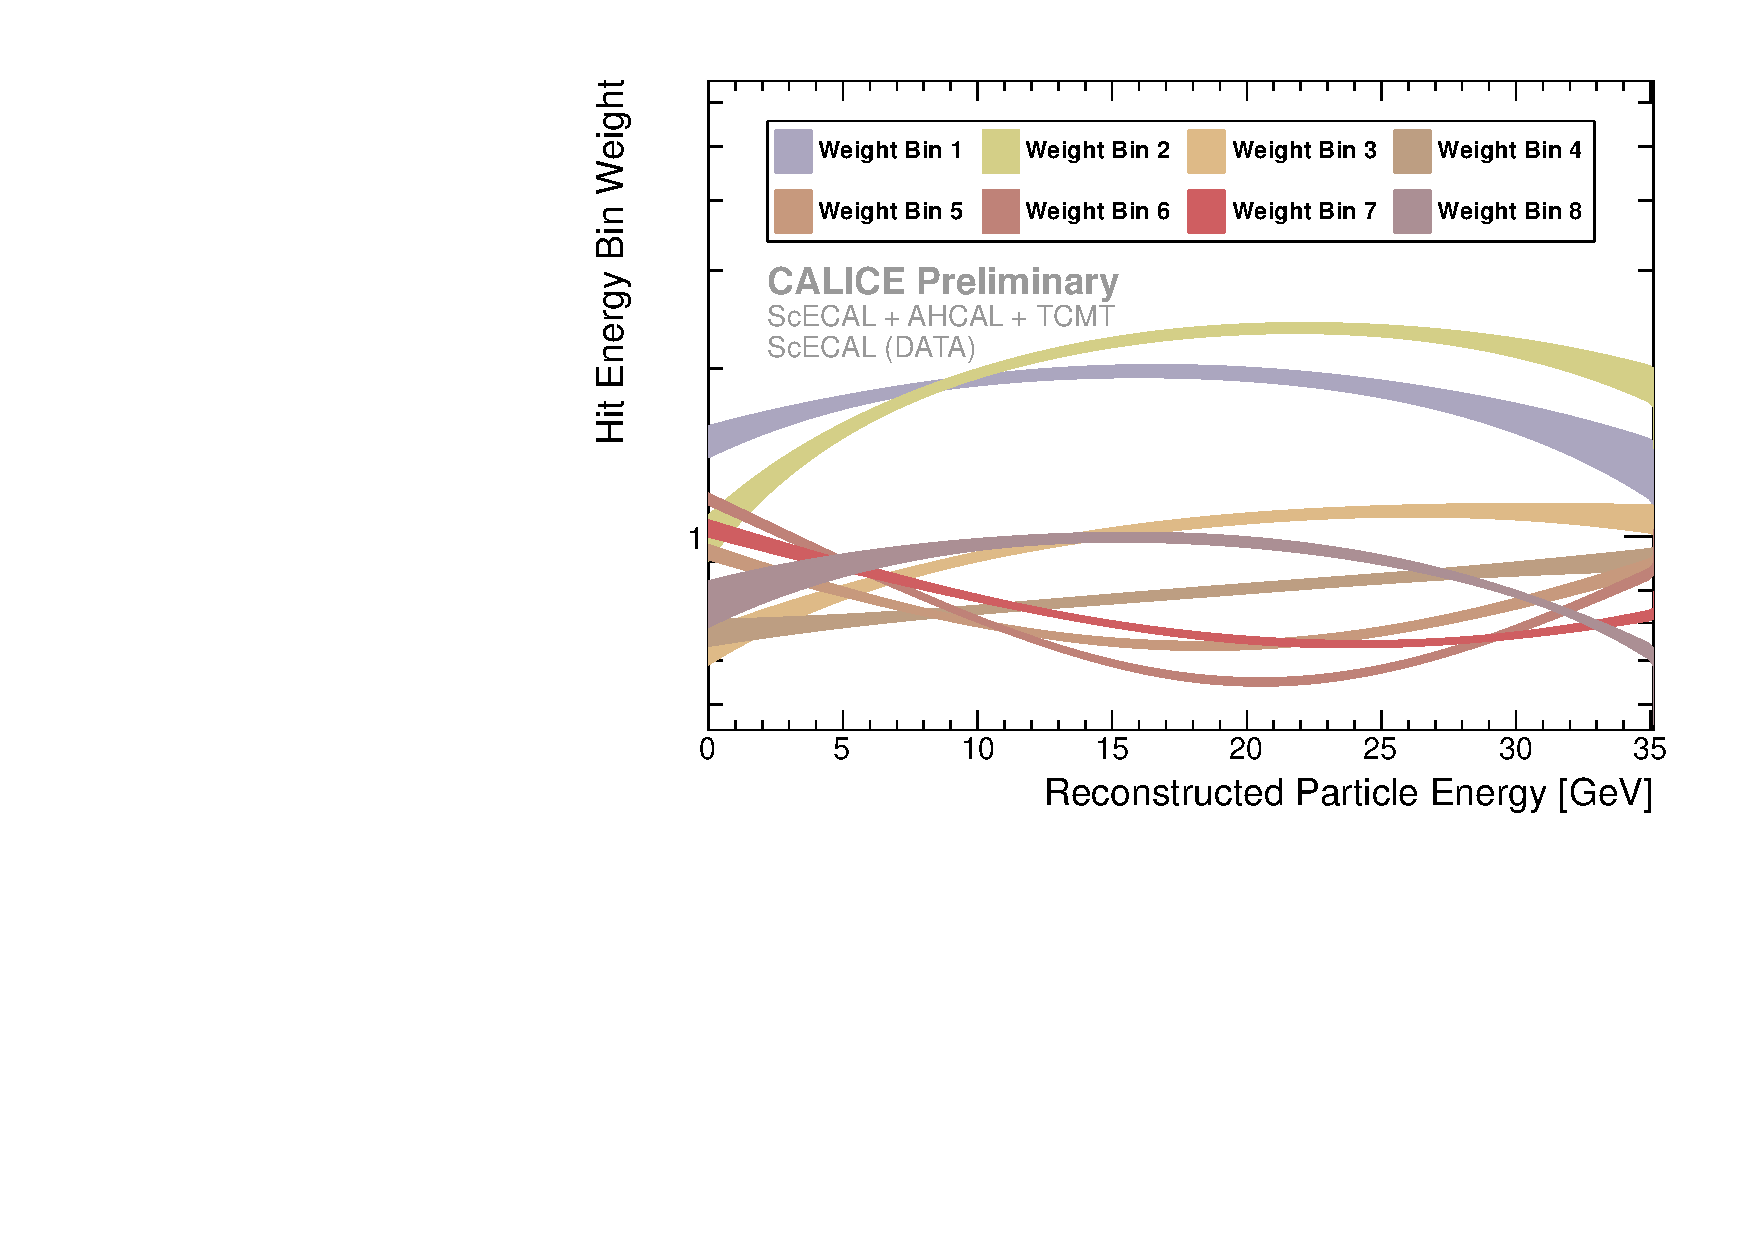
\includegraphics[width=0.5\textwidth,page=1]{fig/pion/SC/weights_DATA.pdf}}\hfill
	\subfigure[AHCAL bin weights as a function of energy] {\includegraphics[width=0.5\textwidth,page=2]{fig/pion/SC/weights_DATA.pdf}}
	\subfigure[ScECAL bin weights for selected energies] {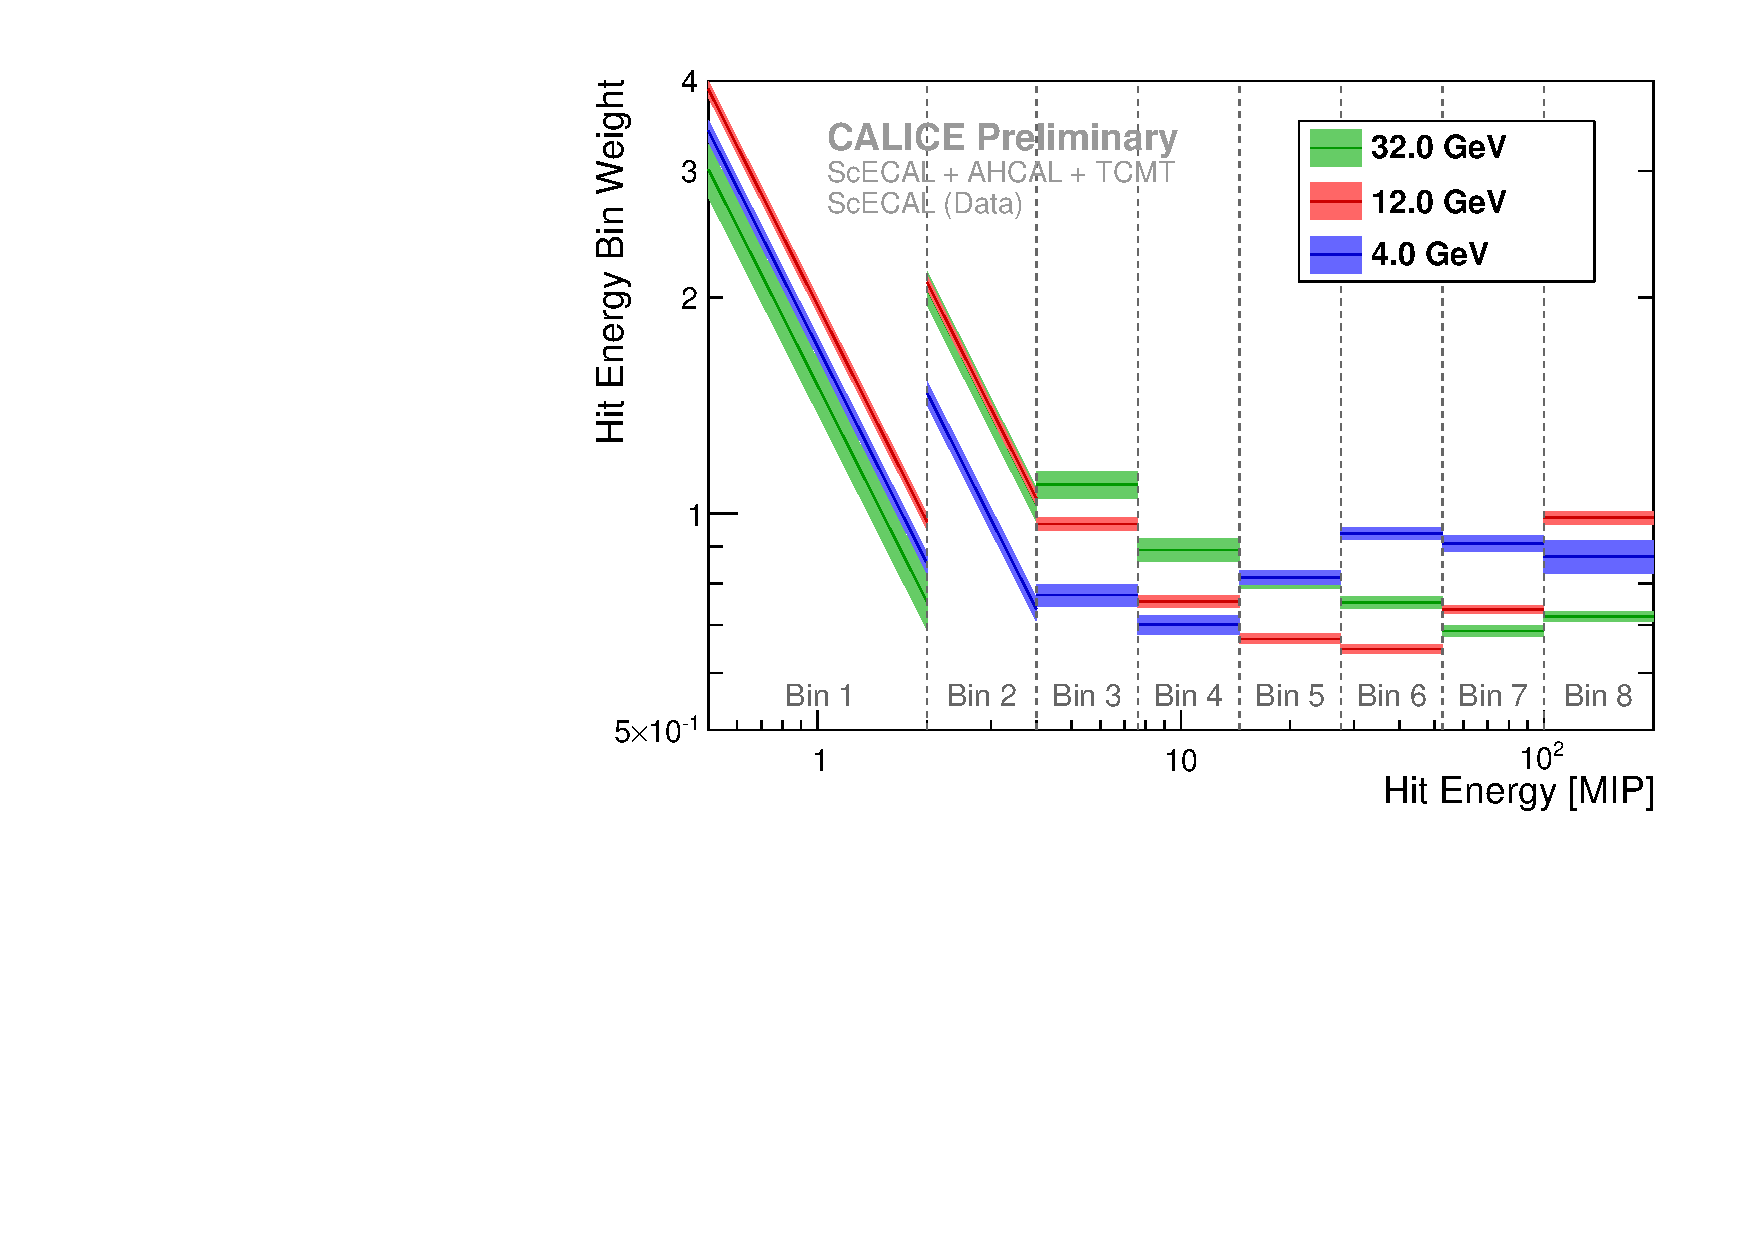
\includegraphics[width=0.5\textwidth,page=1]{fig/pion/SC/binWeights_DATA.pdf}}\hfill
	\subfigure[AHCAL bin weights for selected energies] {\includegraphics[width=0.5\textwidth,page=2]{fig/pion/SC/binWeights_DATA.pdf}}
	
	\caption{Hit energy bin weights as a function of beam energy, optimised from data runs. In \textbf{(c)} and \textbf{(d)}, the hit energy dependent weights of the first two bins correspond to a $\nicefrac{1}{E}$ dependence and thus a counting of hits in these bins. The width of each plotted line indicates the weight uncertainty propagated from the parameter errors.}
	\label{fig:SCweightsData}
\end{figure}

Applying the weights shown in \autoref{fig:SCweightsData} to the dataset yields an improvement in energy resolution as shown in \autoref{fig:ClassicVsSC}. Iterations of software compensation reconstruction using the previous result as $E_\text{est.}$ do not further improve the energy resolution.  The correlation between standard and software compensation reconstruction shows a clear non-linearity in the central part of the reconstructed energies, causing events with a high hadronic fraction, and thus lower standard reconstructed energy, to be shifted up in software compensation reconstruction. Likewise events with above average electromagnetic shower content, and thus too high standard reconstructed energy, are shifted down when reconstructed with the software compensation reconstruction.
\begin{figure}[htbp]
	\subfigure[Reconstructed energy spectra for standard and software compensation reconstruction.] {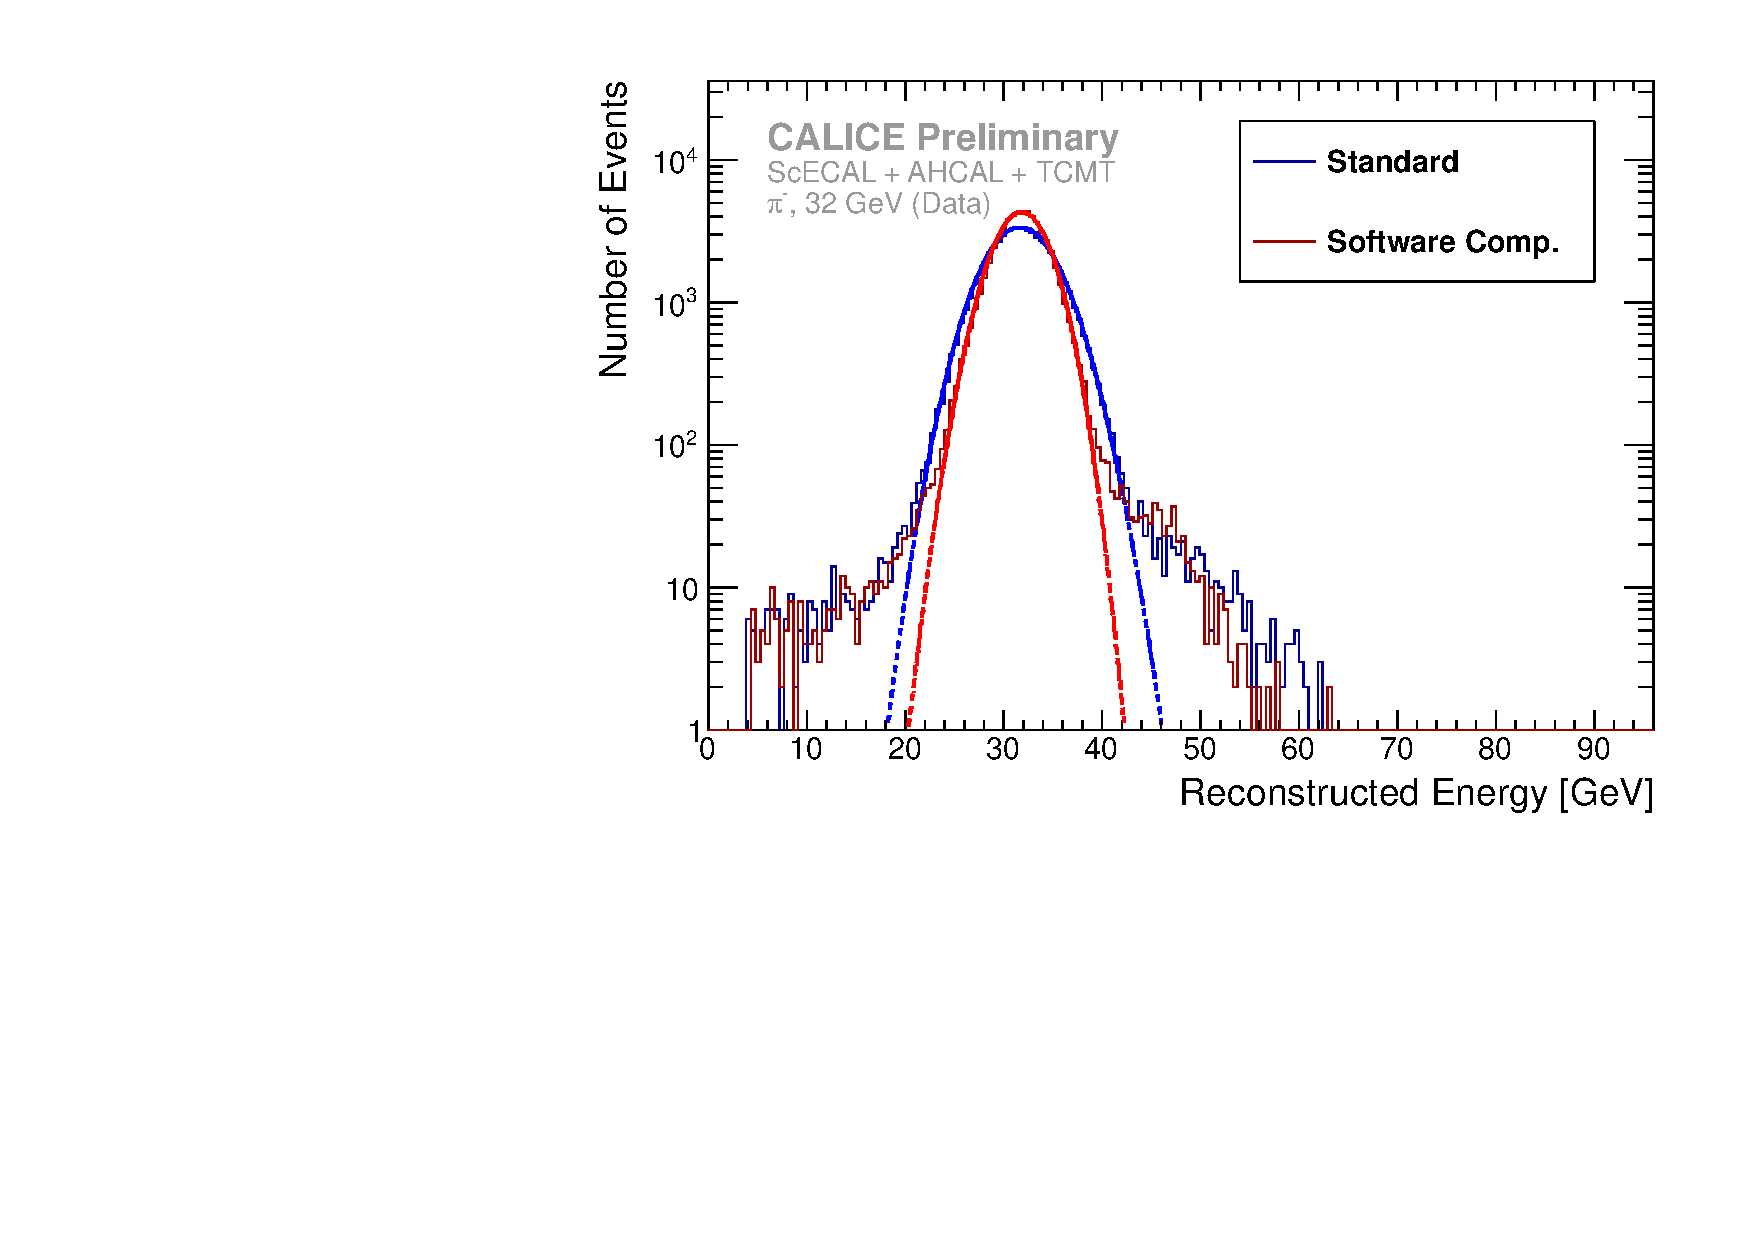
\includegraphics[width=0.5\textwidth]{fig/pion/SC/ERec_classic_SC_560474_data.pdf}}\hfill
	\subfigure[Correlation standard vs. software compensation reconstructed energy.] {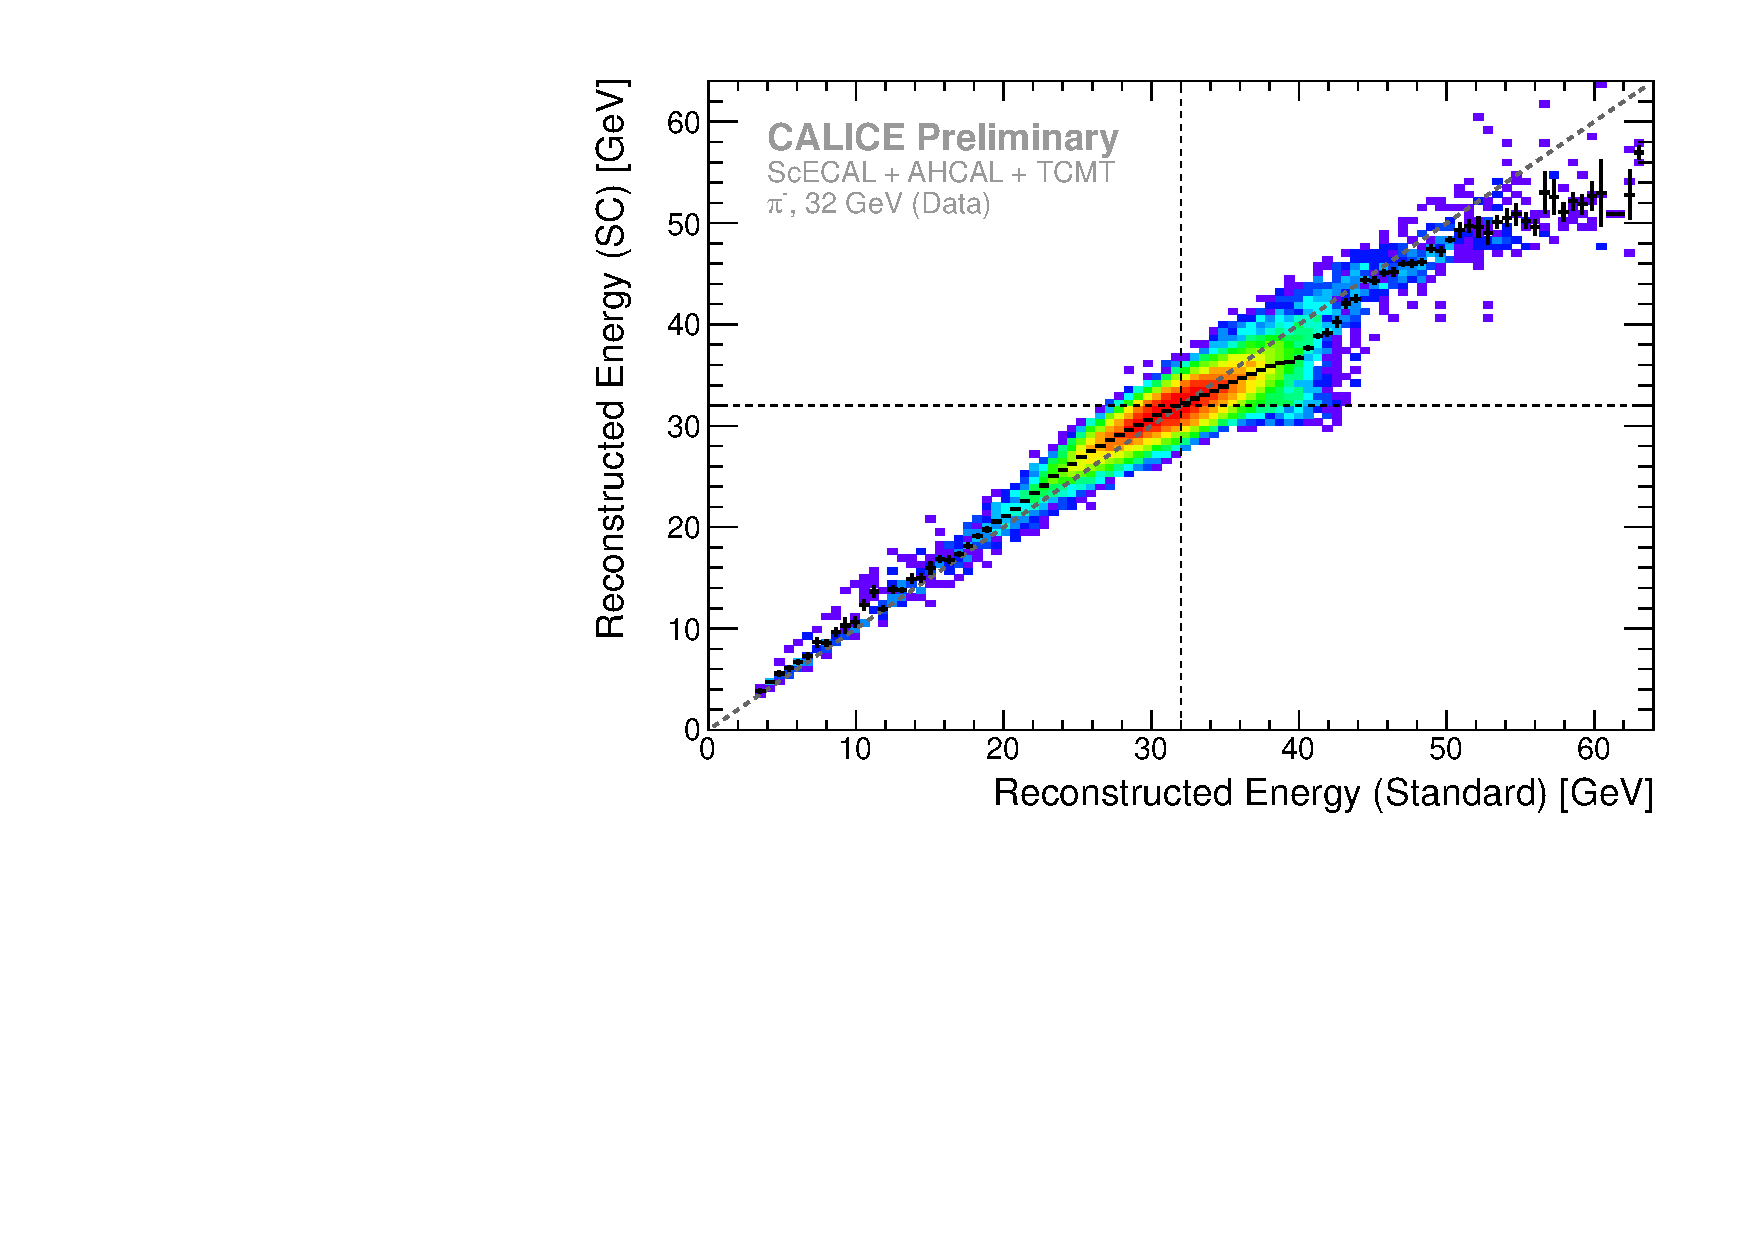
\includegraphics[width=0.5\textwidth]{fig/pion/SC/ERec_corr_560474_data.pdf}}
	
	\caption{Reconstructed energy in standard and software compensation reconstruction for data run 560474 (32\,GeV\piminus). The black markers in the correlation plot show the profile of mean software compensation reconstructed energy for bins in standard reconstruction energy. The black dashed lines in the correlation plot indicate the beam energy of the run.}
	\label{fig:ClassicVsSC}
\end{figure}

The identical procedure of reconstructing energies and optimising weight parameter is applied on simulated events. The dependence of bin weight to beam energy compared between data and simulation is shown in \autoref{fig:SCWeightsDataVsMC} for selected bins. All used simulation physics lists agree with each other within parameter uncertainties. While the AHCAL generally shows reasonable agreement between weights derived from data and simulations in all bins, the ScECAL shows discrepancies especially for the first two bins and the highest hit energy bin. The TCMT weight also has a large discrepancy between data and simulations, although mostly for low beam energies in which TCMT depositions are expected to be minimal.


\begin{figure}[htbp]
	\subfigure[ScEcal Bin 1\label{fig:weight_scecal_bin1}] {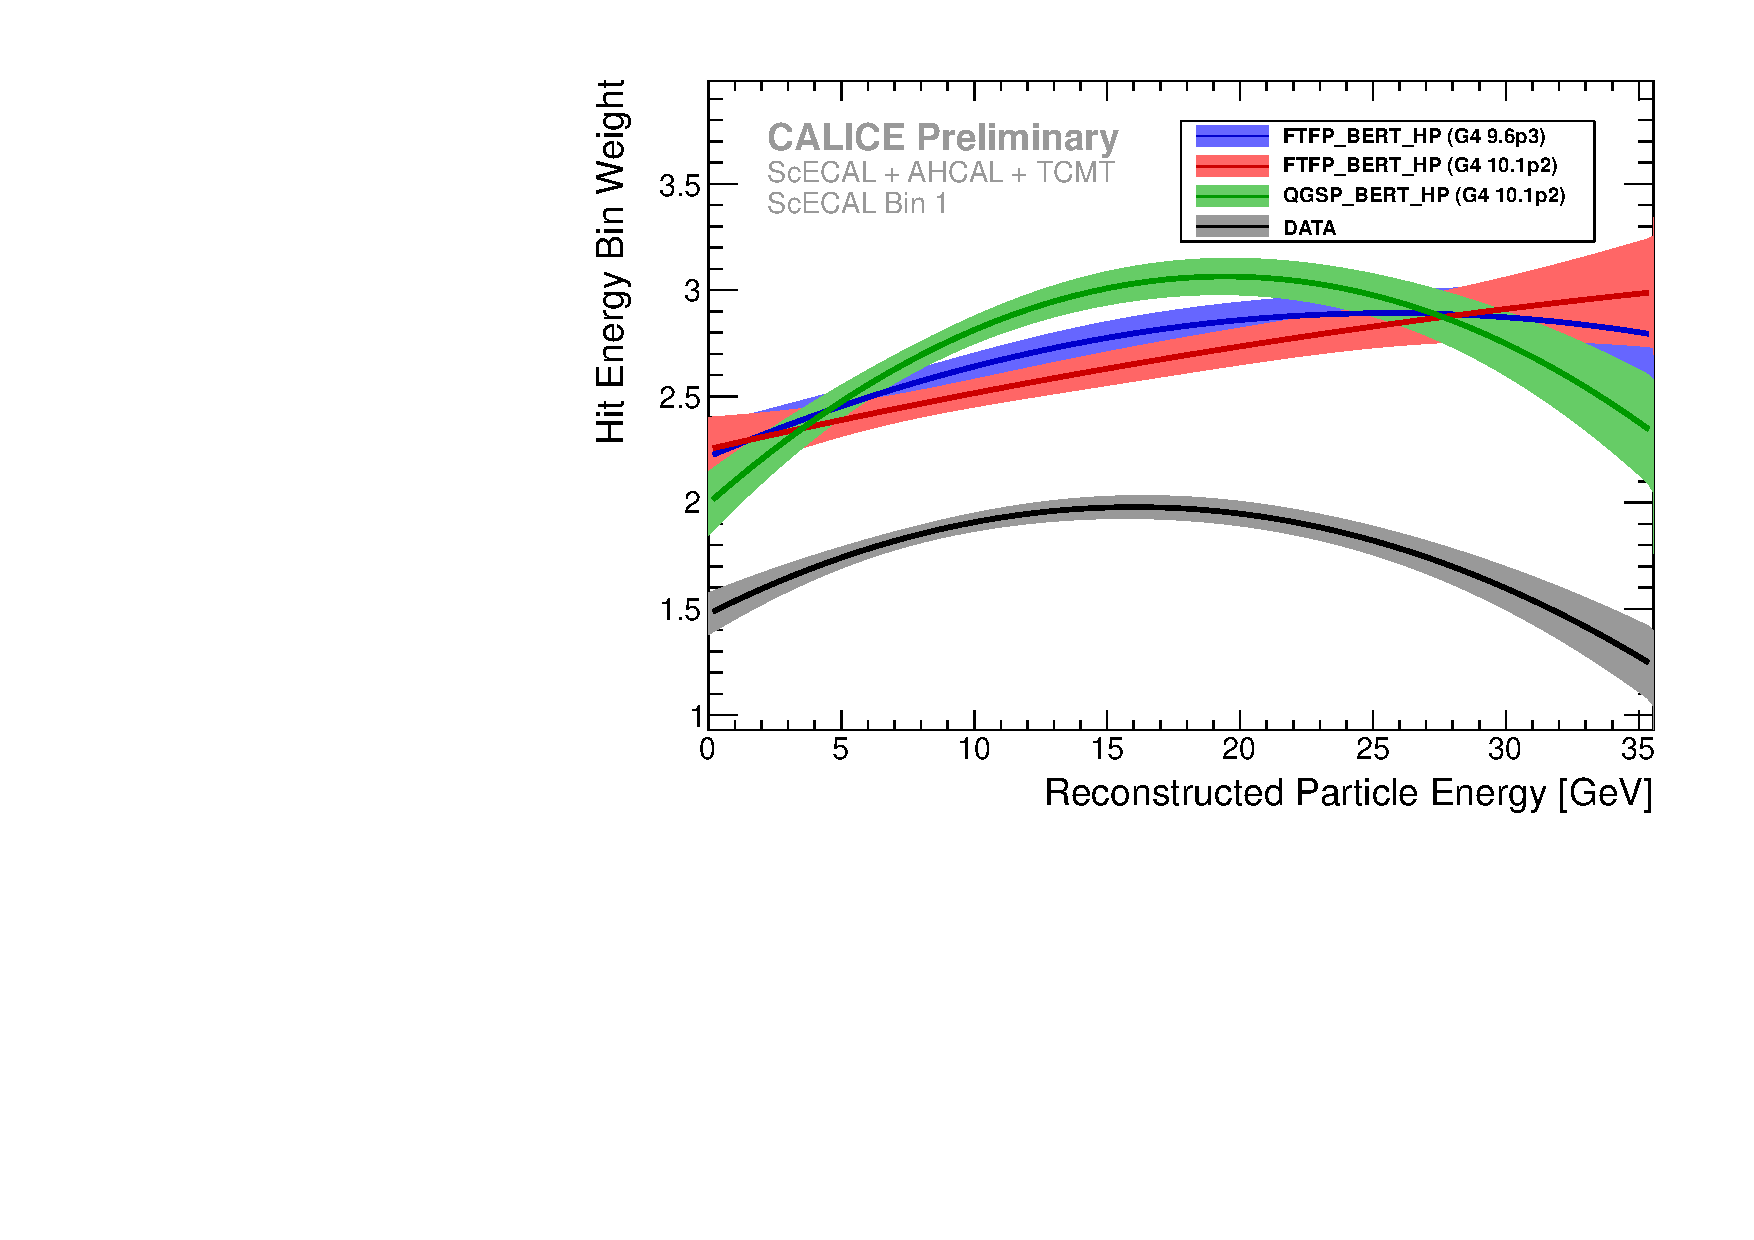
\includegraphics[width=0.5\textwidth,page=1]{fig/pion/SC/weightsSC.pdf}}\hfill
	\subfigure[ScEcal Bin 4] {\includegraphics[width=0.5\textwidth,page=4]{fig/pion/SC/weightsSC.pdf}}
	\subfigure[ScEcal Bin 8\label{fig:weight_scecal_bin8}] {\includegraphics[width=0.5\textwidth,page=8]{fig/pion/SC/weightsSC.pdf}}\hfill
	\subfigure[AHCAL Bin 3] {\includegraphics[width=0.5\textwidth,page=11]{fig/pion/SC/weightsSC.pdf}}
	
	\caption{Hit energy bin weights as a function of beam energy for data and different simulations. The width of each plotted line indicates the weight uncertainty propagated from the parameter errors. Low and high hit energy bin weights are not well reproduced in the ScECAL.}
	\label{fig:SCWeightsDataVsMC}
\end{figure}

The ScECAL pion hit energy spectra show similar behaviour to the electron hit spectra discussed in \autoref{sec:scecalvalidation}, as in high tails of the ScECAL hit energy spectrum being overestimated in simulation, especially for high beam energies. 

Optimising the software compensation weights on data runs reconstructed with a shifted saturation scale in the ScECAL (as described in \autoref{sec:scecalvalidation}) shows only a very small influence on the optimised weights. Optimising weights from simulations with adjusted air gaps between ScECAL layers (also as described in \autoref{sec:scecalvalidation}) yields bin weights with small but significant differences to the standard simulation.

The averaged summed deposition per event for each bin is investigated in order to understand the observed differences in the weights, as shown in \autoref{fig:hitenergyBinsPion}. The highest hit energy bin in the ScECAL has around twice of the mean deposition in simulation compared to data, with significant differences showing from the sixth bin. For lower energies the effect is less pronounced. In the AHCAL all bins show reasonable agreement between data and simulation, with smaller overestimations in the highest hit energy bin.

\begin{figure}[htbp]
\begin{center}
	\subfigure[ScECAL, Run 560506 (4\,GeV)] {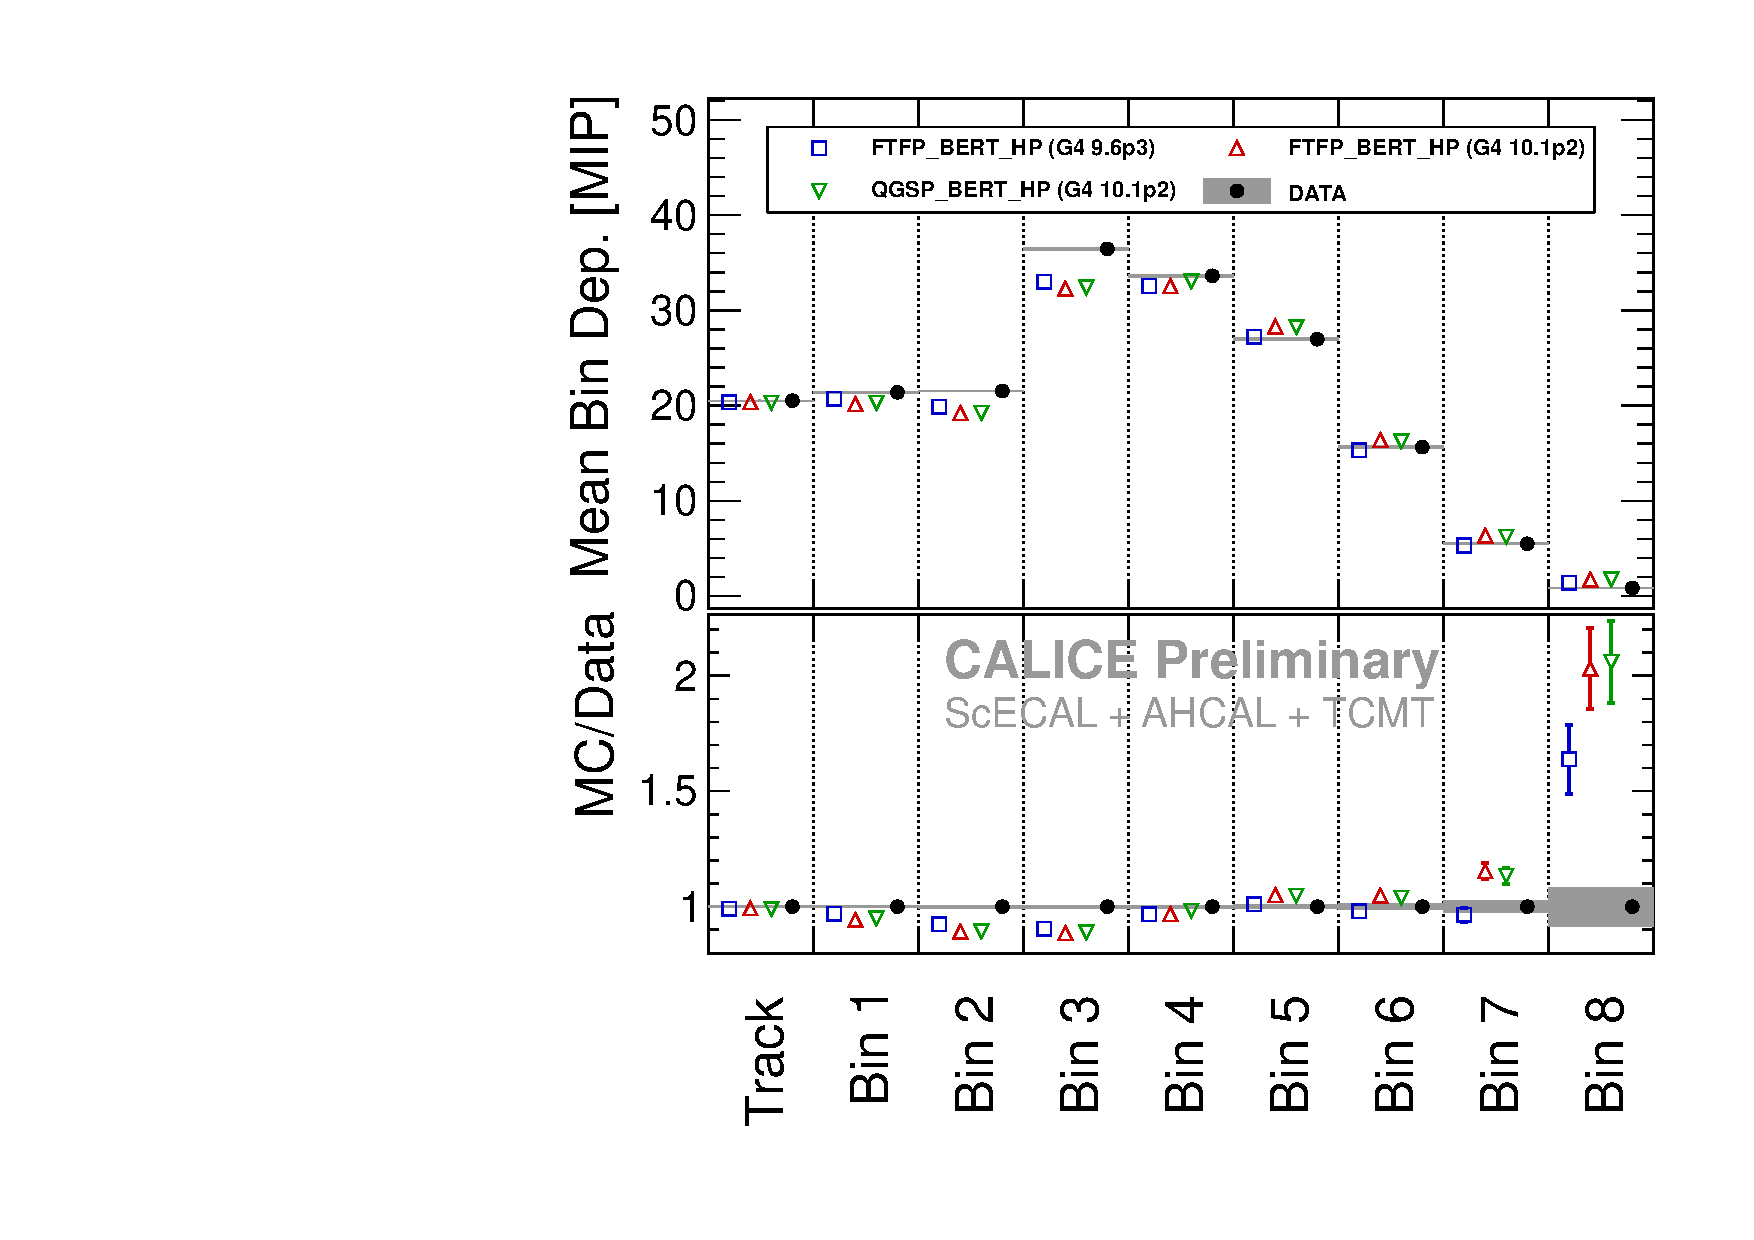
\includegraphics[width=0.5\textwidth,page=1]{fig/pion/SC/meanBinEnergy.pdf}}\hfill
	\subfigure[AHCAL, Run 560506 (4\,GeV)] {\includegraphics[width=0.5\textwidth,page=6]{fig/pion/SC/meanBinEnergy.pdf}}
	\subfigure[ScECAL, Run 560474 (32\,GeV)] {\includegraphics[width=0.5\textwidth,page=5]{fig/pion/SC/meanBinEnergy.pdf}}\hfill
	\subfigure[AHCAL, Run 560474 (32\,GeV)] {\includegraphics[width=0.5\textwidth,page=10]{fig/pion/SC/meanBinEnergy.pdf}}
\end{center}
	\caption{Averaged energy deposition sum per hit energy bin per event for data and simulations in ScECAL and AHCAL. For most entries the statistical error is smaller than the used markers.}
	\label{fig:hitenergyBinsPion}
\end{figure}

The observed differences in mean hit energy per bin (and thus hit energy spectra) do not sufficiently explain the differences in optimised software compensation weights on their own. Although the highest ScECAL hit energy bin shows discrepancies between data and simulation for all beam energies, its bin weight is only different in the central part of the beam energies (see \autoref{fig:weight_scecal_bin8}). Likewise the mean energy sum in the first ScECAL hit energy bin is well described for all energies, but the corresponding bin weights are not (see \autoref{fig:weight_scecal_bin1}).

Remaining instrumental and shower modelling effects could affect the optimised weights even in hit energy ranges where the observed hit energy spectra match reasonably between data and simulation, as bin weights are necessarily anti-correlated to conserve the mean reconstructed energy. Possible instrumental effects are covered by the systematic uncertainties given, so we consider the possibility that the modelling of the pion shower structure is imperfect, especially in high-Z absorbers and on the granularity scale that is studied here.
%\newpage
\section{Results}
This section describes the results obtained from using the techniques described above in comparison between data and simulations, starting with longitudinal profiles of pion showers to energy reconstruction and linearity of the system as well as energy resolution with standard and software compensation reconstruction.
\subsection{Profiles}\label{sec:profiles}
The mean longitudinal profile of all pion shower events passing the event selection for 32\,GeV beam energy is shown in \autoref{fig:profile_long_full}. The low mean deposition in the first five layers is a consequence of the event selection (FHI layer \textgreater 5). The low mean deposition in the last AHCAL layers points to good average shower containment even without including the TCMT layers. The general shape of the profile is well described by all physics lists, including the dip in responses in the ScECAL around the transition region between the ScECAL and AHCAL. \geant with the FTFP\_BERT physics lists shows a peak in the ratio to data around layer 5 which is not present for QGSP\_BERT\_HP. All studied simulations overestimate the mean depositions by around 5\% regardless of beam energy, as already noted in \autoref{sec:energyrecoclassic}. This difference is larger than the systematic uncertainty on the MIP calibration or saturation effects.
\begin{figure}[htbp]
\begin{center}
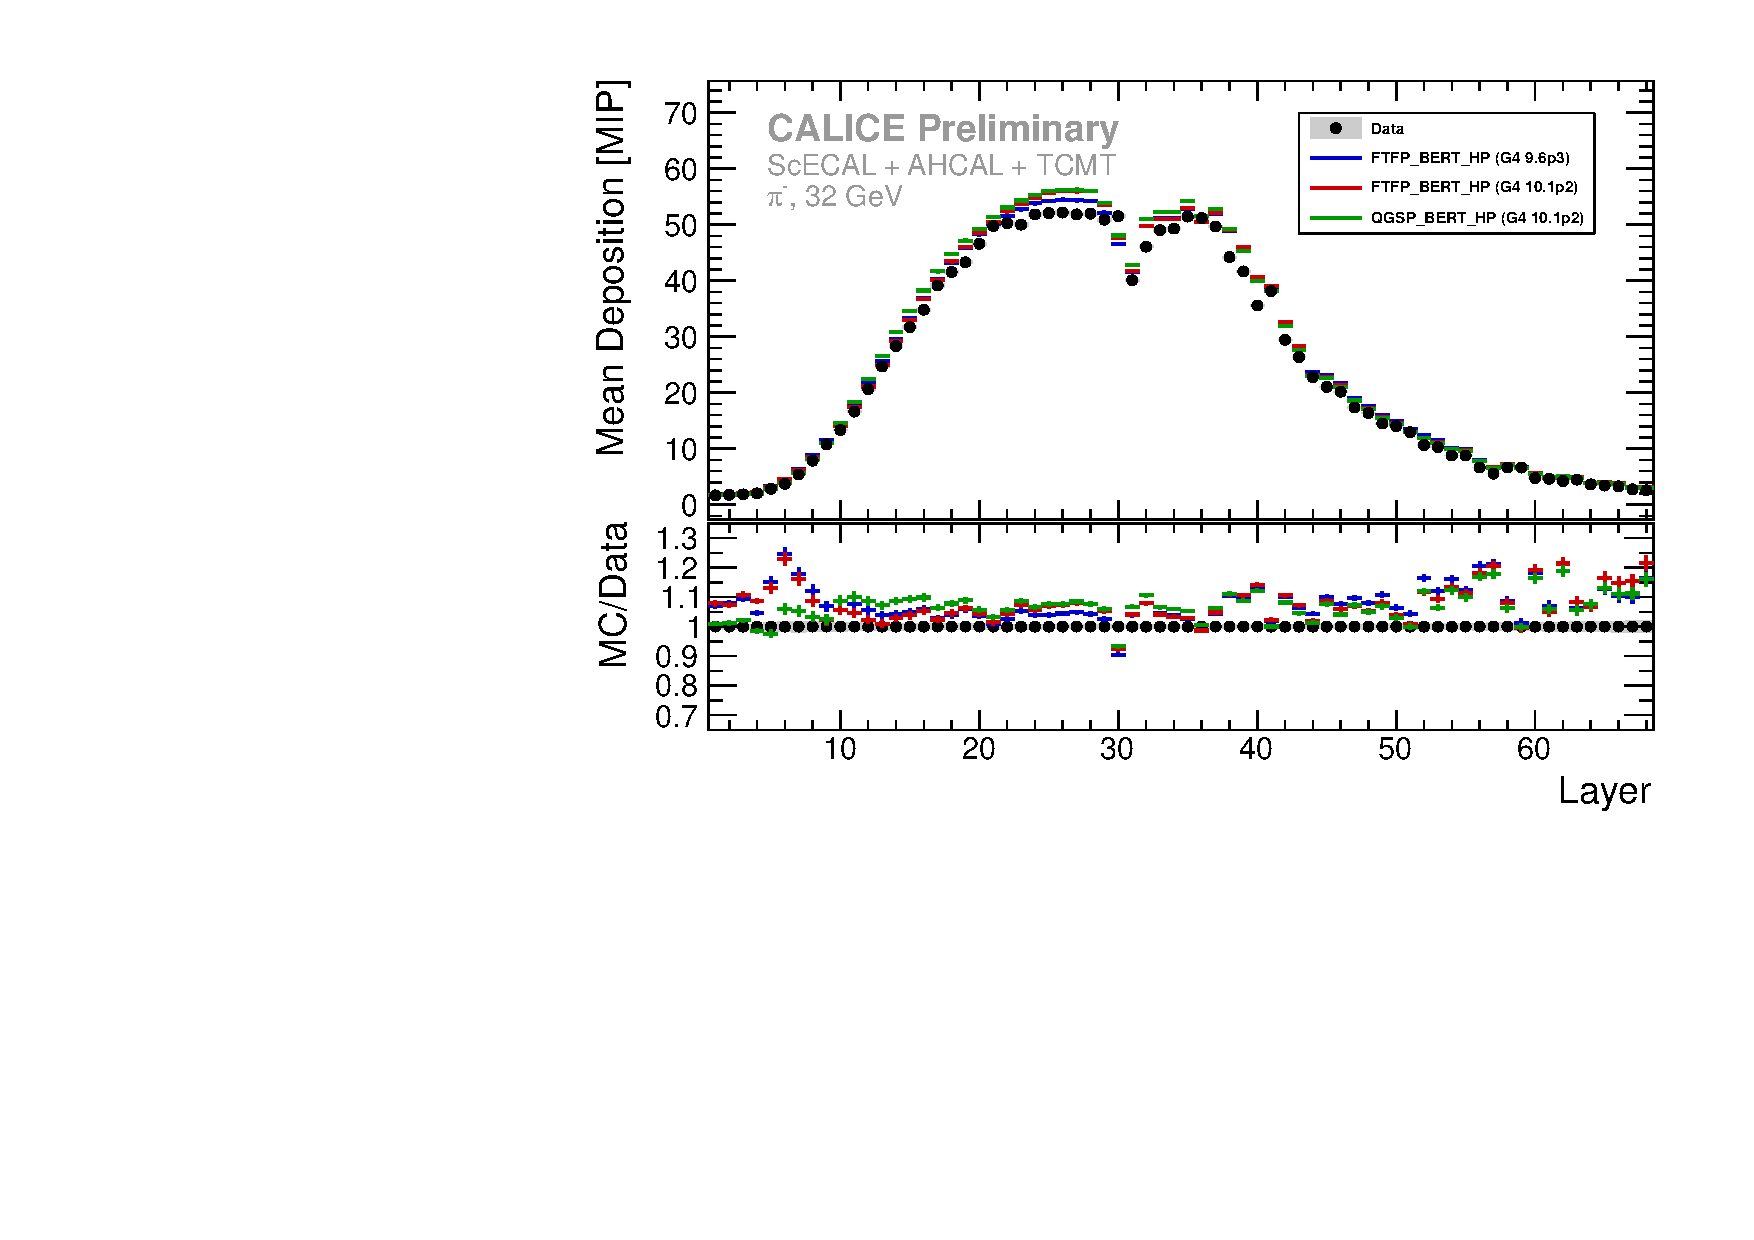
\includegraphics[width=0.8\textwidth]{fig/pion/results/out_profileLongitudinal_560474.pdf}
\caption{Averaged longitudinal shower profile for 32\,GeV \piminus\ events in data and different simulation physics lists. Depositions in the ScECAL are shown in layers 1--30, layers 31--68 are AHCAL layers.}
\label{fig:profile_long_full}
\end{center}
\end{figure}

The longitudinal shower profiles from shower start are shown in \autoref{fig:profile_long_fhi}, separately for showers starting in the ScECAL and in the AHCAL. For events with reconstructed shower start in the ScECAL, the shower profiles predicted by the FTFP\_BERT and QGSP\_BERT simulation models vary significantly, under and overestimating depositions compared to data in different layers, especially for high beam energies. Most of the data points lie between the predictions of the different physics lists used. FTFP\_BERT\_HP in \geant 10.1p2 shows slightly longer showers than \geant 9.6p3.

In events with reconstructed FHI layer in the AHCAL the examined simulation models agree well with each other. The agreement between data and simulation is on a similar level, with similar features in the ratio, as in \cite{CAN48}. In the AHCAL FTFP\_BERT\_HP shows slightly shorter showers in \geant 10.1p2 than in \geant 9.6p3, opposite to the behaviour in the ScECAL.

\begin{figure}[htbp]
\begin{center}
	\subfigure[Shower start in ScECAL layer 5--16.] {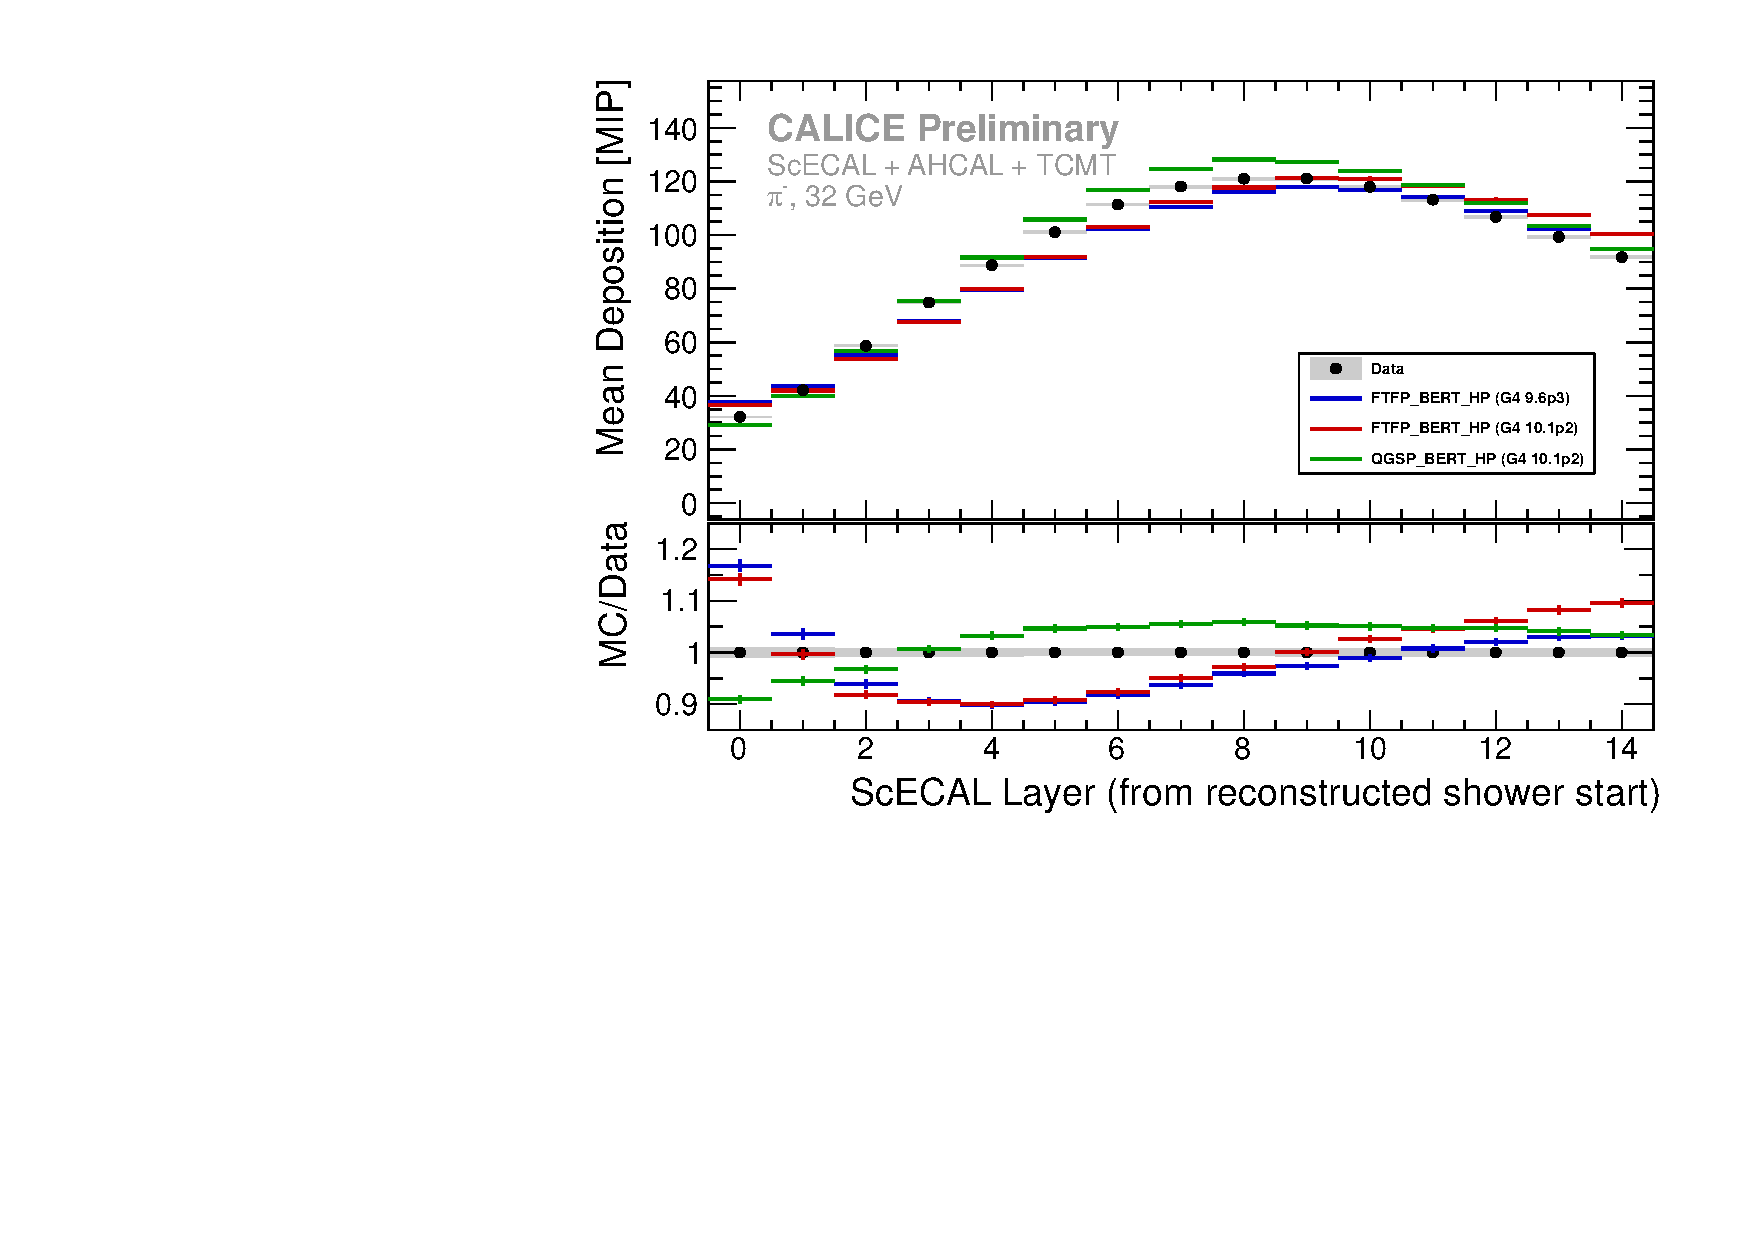
\includegraphics[width=0.5\textwidth]{fig/pion/results/out_profileLongitudinalECALFHI_560474.pdf}}\hfill
	\subfigure[Shower start in AHCAL layer 0--10.] {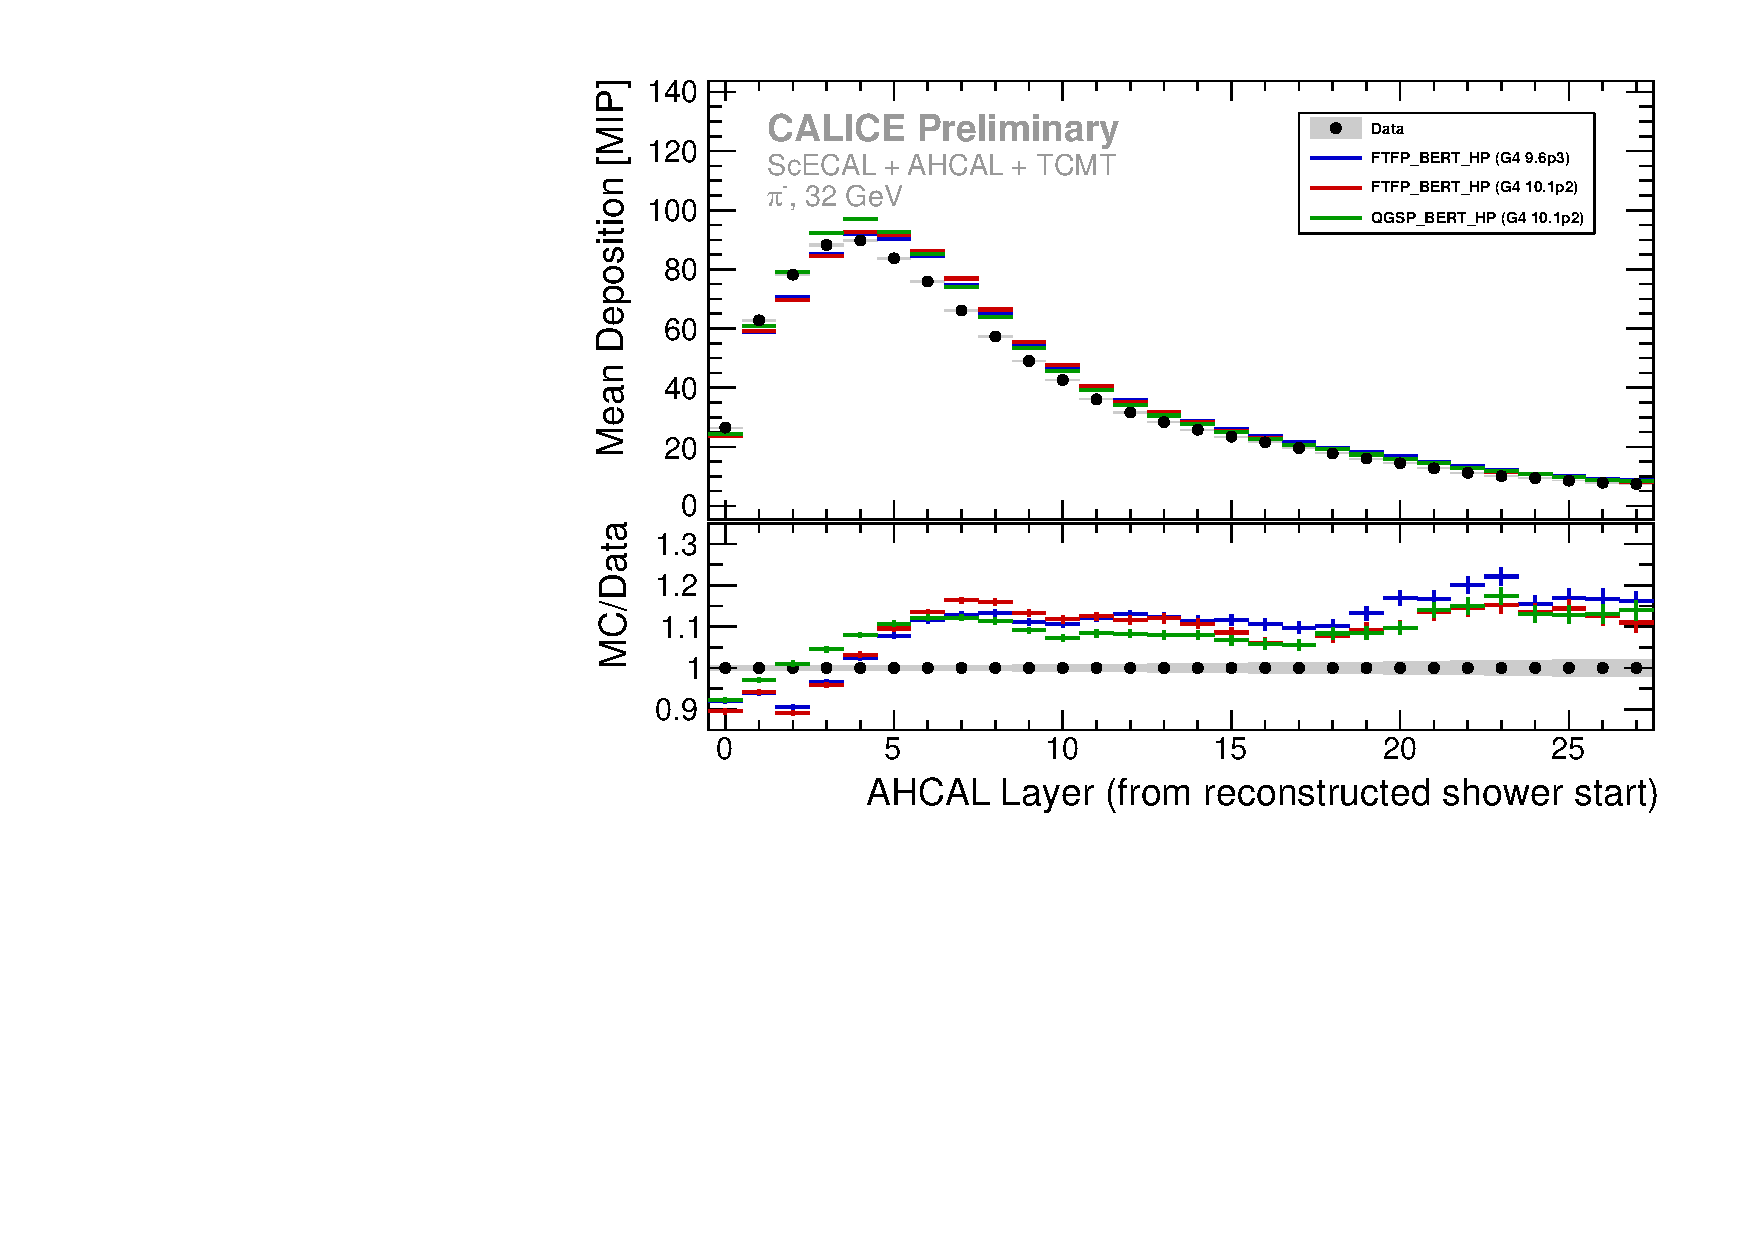
\includegraphics[width=0.5\textwidth]{fig/pion/results/out_profileLongitudinalHCALFHI_560474.pdf}}
\end{center}
	\caption{Averaged longitudinal shower profile for 32\,GeV \piminus\ events in data and different simulation physics lists. Depositions are plotted as function of distance to reconstructed FHI layer.}
	\label{fig:profile_long_fhi}
\end{figure}

\subsection{Energy reconstruction and linearity}
For each event the particle energy is reconstructed with the techniques described in \autoref{sec:energyreco}, without use of the known beam energy. For each run the spectrum of obtained reconstructed energies is fitted with a Novosibirsk function, of which the response and resolution are calculated using Monte-Carlo integration as explained in \cite{CAN49}.

Data and all simulation physics lists are reconstructed with the parameters optimised from their own datasets. A systematic uncertainty of 1\% on the MIP scale is added in quadrature to the negligible statistical error of the response. The systematic uncertainty from the modified air gap in simulations and the shifted saturation scales in data is negligible. 
%[syst. uncertainty is fully correlated in simulation by construction, semi-correlated in data.] 
The residual is defined as the relative deviation of the mean reconstructed energy from the known beam energy. 

The mean reconstructed energies in data agree very well with the beam energy with all deviations better than 3\%, as shown in \autoref{fig:pion_linearity}.  
The reconstructed energy observed in simulations shows a small non-linearity with no deviation from the beam energy exceeding 5\%. 

Reconstructing the particle energy using the software compensation scheme described in \autoref{sec:energyrecosc}, the linearity of data and simulated events is better than 3\%. 
\begin{figure}[htbp]
\begin{center}
	\subfigure[Standard Reconstruction] {\includegraphics[width=0.5\textwidth,page=2]{fig/pion/results/pion_linearity.pdf}}\hfill
	\subfigure[Software Compensation Reconstruction] {\includegraphics[width=0.5\textwidth,page=4]{fig/pion/results/pion_linearity.pdf}}
\end{center}
	\caption{Residual of mean fitted reconstructed energy over beam energy in data and different simulation physics lists. }
	\label{fig:pion_linearity}
\end{figure}

\subsection{Energy resolution}
The resolution of each run is calculated from the width and mean of the Novosibirsk function fitted to the reconstructed energy spectrum, using reconstruction parameters as described in the previous section. For simulated runs, the difference in resolution between standard simulation and simulation with modified airgap is taken as fully correlated systematic uncertainty. Shifting the saturation scale has no significant effect on the reconstructed energy resolution in data and is thus omitted as a systematic uncertainty. The statistical uncertainty on each resolution point is small.

In standard energy reconstruction, the data points are generally well described by the simulations, see \autoref{fig:pion_resolution}. QGSP\_BERT\_HP produces the best agreement with data while the FTFP\_BERT\_HP samples show deviations either in the low or high beam energy region of the sample.

Software compensation leads to a relative improvement of data point resolutions between 10--20\% (2--3\% absolute), depending on beam energy, see \autoref{fig:pion_resolution}.
The resolution of the simulated samples agrees between physics lists when using software compensation reconstruction, but generally and significantly overestimates the achievable resolution improvements by relative 5--10\% compared to data as shown in \autoref{fig:pion_reso_sc_ratio}. The used calorimeter system combining several readout granularities, samplings and absorber materials is reasonably described in simulations, even when complex energy reconstructions, utilising the detailed structure of individual showers, are employed. 

\begin{figure}[htbp]
\begin{center}
	\subfigure[Energy Resolutions\label{fig:pion_resolution}] {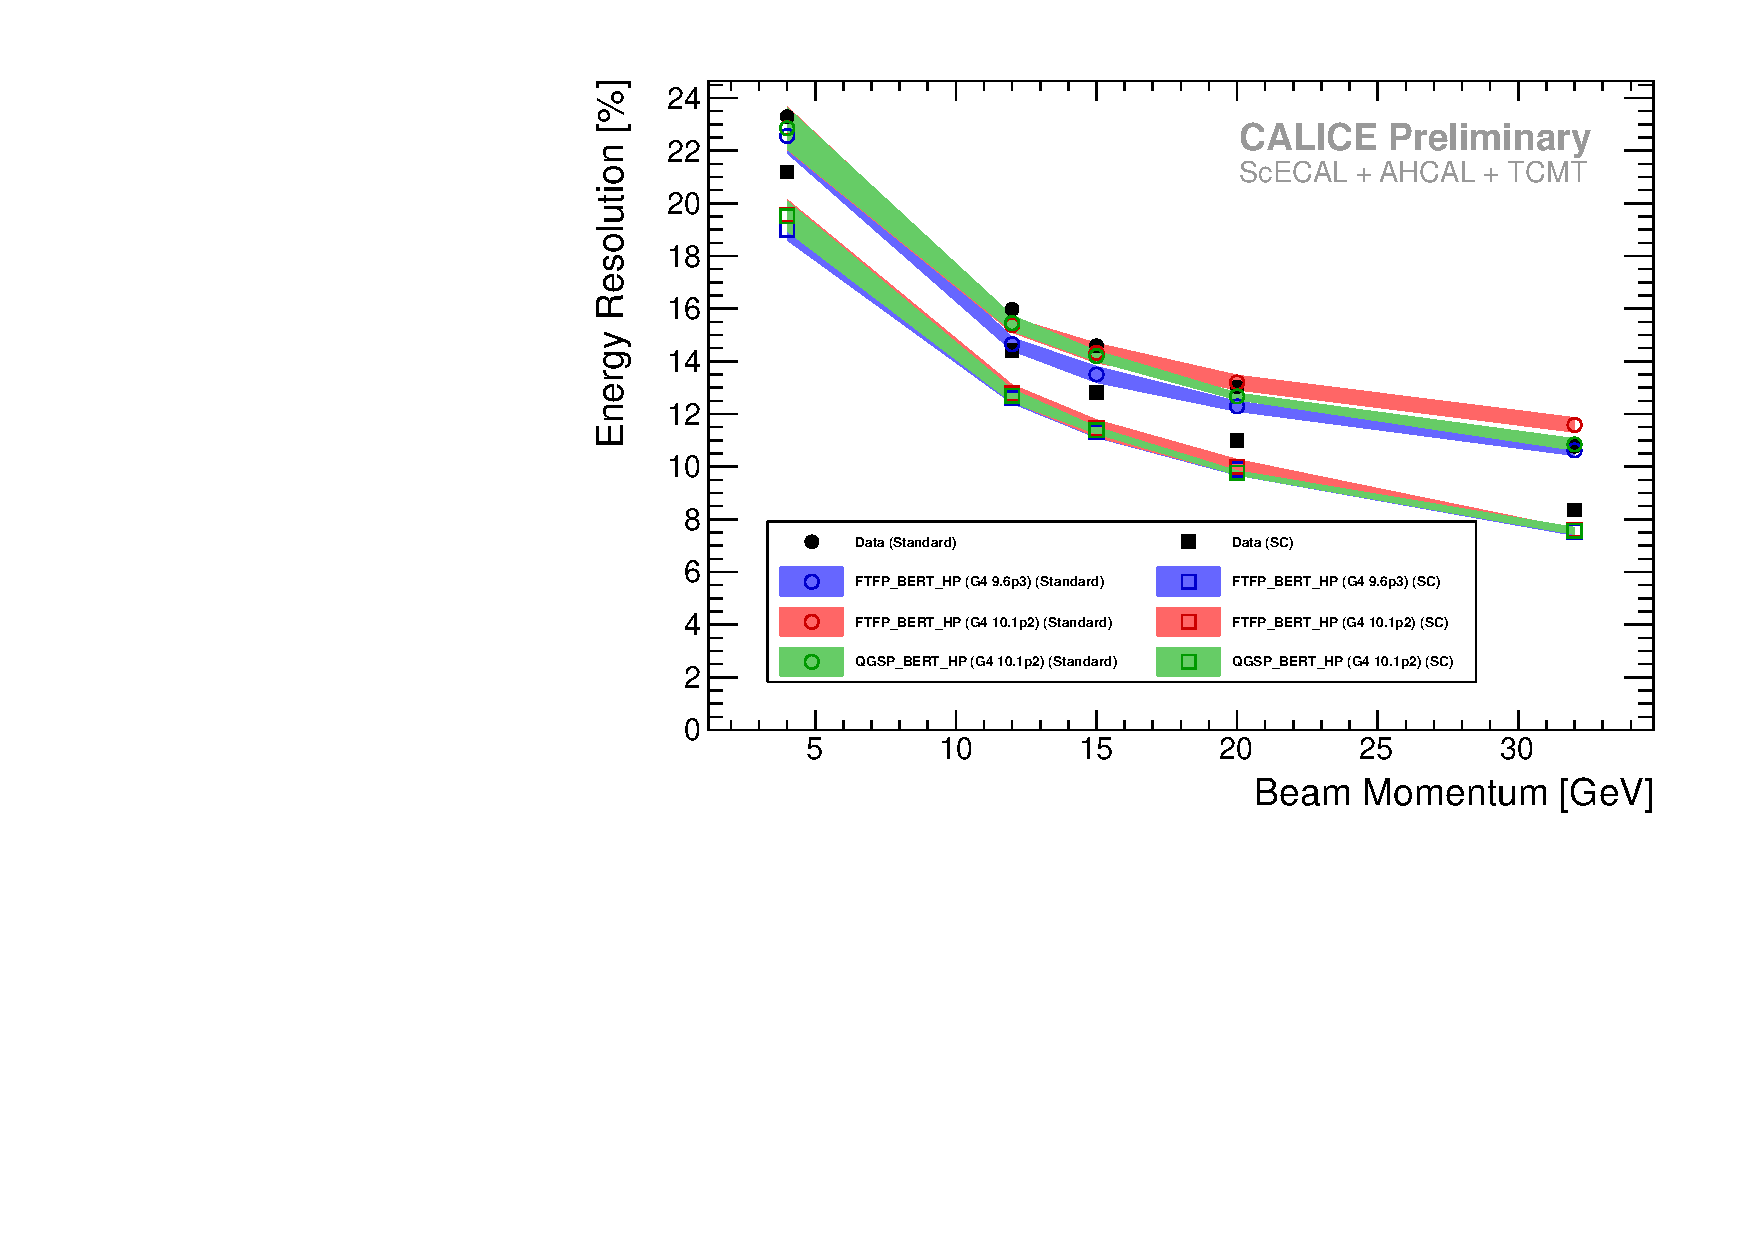
\includegraphics[width=0.5\textwidth,page=1]{fig/pion/results/pion_resolution.pdf}}\hfill
	\subfigure[Resolution improvement with software compensation\label{fig:pion_reso_sc_ratio}] {\includegraphics[width=0.5\textwidth,page=3]{fig/pion/results/pion_resolution.pdf}}
\end{center}
	\caption{Reconstructed energy resolution as a function of beam energy in data and different simulation physics lists for standard and software compensation reconstruction. All plotted values are tabulated in \autoref{table:pionresolution}.}
	\label{fig:pion_resolution_plots}
\end{figure}

\autoref{fig:pion_resolution_vs_ahcal} compares the energy resolution obtained from data in this analysis to the energy resolutions obtained from \cite{SCPaper}, in which only pion showers with reconstructed FHI layer in the AHCAL are considered. The resolutions obtained for both analyses are in good agreement, indicating that the combined energy reconstruction with different absorber materials and sampling fractions maintains the single pion energy resolution of the calorimeter system.

\begin{figure}[htbp]
\begin{center}
\includegraphics[width=0.8\textwidth,page=4]{fig/pion/results/pion_resolution.pdf}
\caption{Single pion energy resolutions with standard and software compensation reconstruction from the combined ScECAL+AHCAL+TCMT system compared to resolutions obtained from AHCAL+TCMT in \cite{SCPaper}.}
\label{fig:pion_resolution_vs_ahcal}
\end{center}
\end{figure}
\subsection{Applying Software Compensation Weights from Simulation to Data}
To estimate the influence of the deviations in optimised software compensation weights between data and simulations, and to test whether software compensation weights obtained from simulated events can be used to reconstruct data events, \autoref{fig:pion_data_mc_weights} shows the energy resolution and linearity of data runs reconstructed using weights optimised from both data and simulation. Only the simulation weights optimised from QGSP\_BERT\_HP in Geant\,4 10.2p1 are used for this comparison, as the difference between weights of different simulation physics lists is small. Furthermore only the software compensation specific weights $\alpha_i, \beta_i, \gamma$ are used from simulation, while the standard reconstruction weights $w_{\text{ECAL}}, w_{\text{HCAL}}$ are used from data to set the correct energy reconstruction scale (see \autoref{sec:energyrecoclassic}).

Applying software compensation weights obtained from simulations to data events actually improves the energy resolution slightly by relative 1--3\,\%. However the achieved linearity is deteriorated, showing generally larger deviations than for weights derived from data, with fluctuations of magnitude similar as seen in the resolution of 1--4\,\%. Although there are significant differences in the first two and last ScECAL hit energy bin weights between data and simulation, applying weights optimised from simulation onto data events does not deteriorate the energy resolution of the combined system and only very slightly worsens the deviations from linearity to still acceptable $\leq 4\,\%$ in the energy range examined in this analysis.
\begin{figure}[htbp]
\begin{center}
	\subfigure[Energy Resolutions] {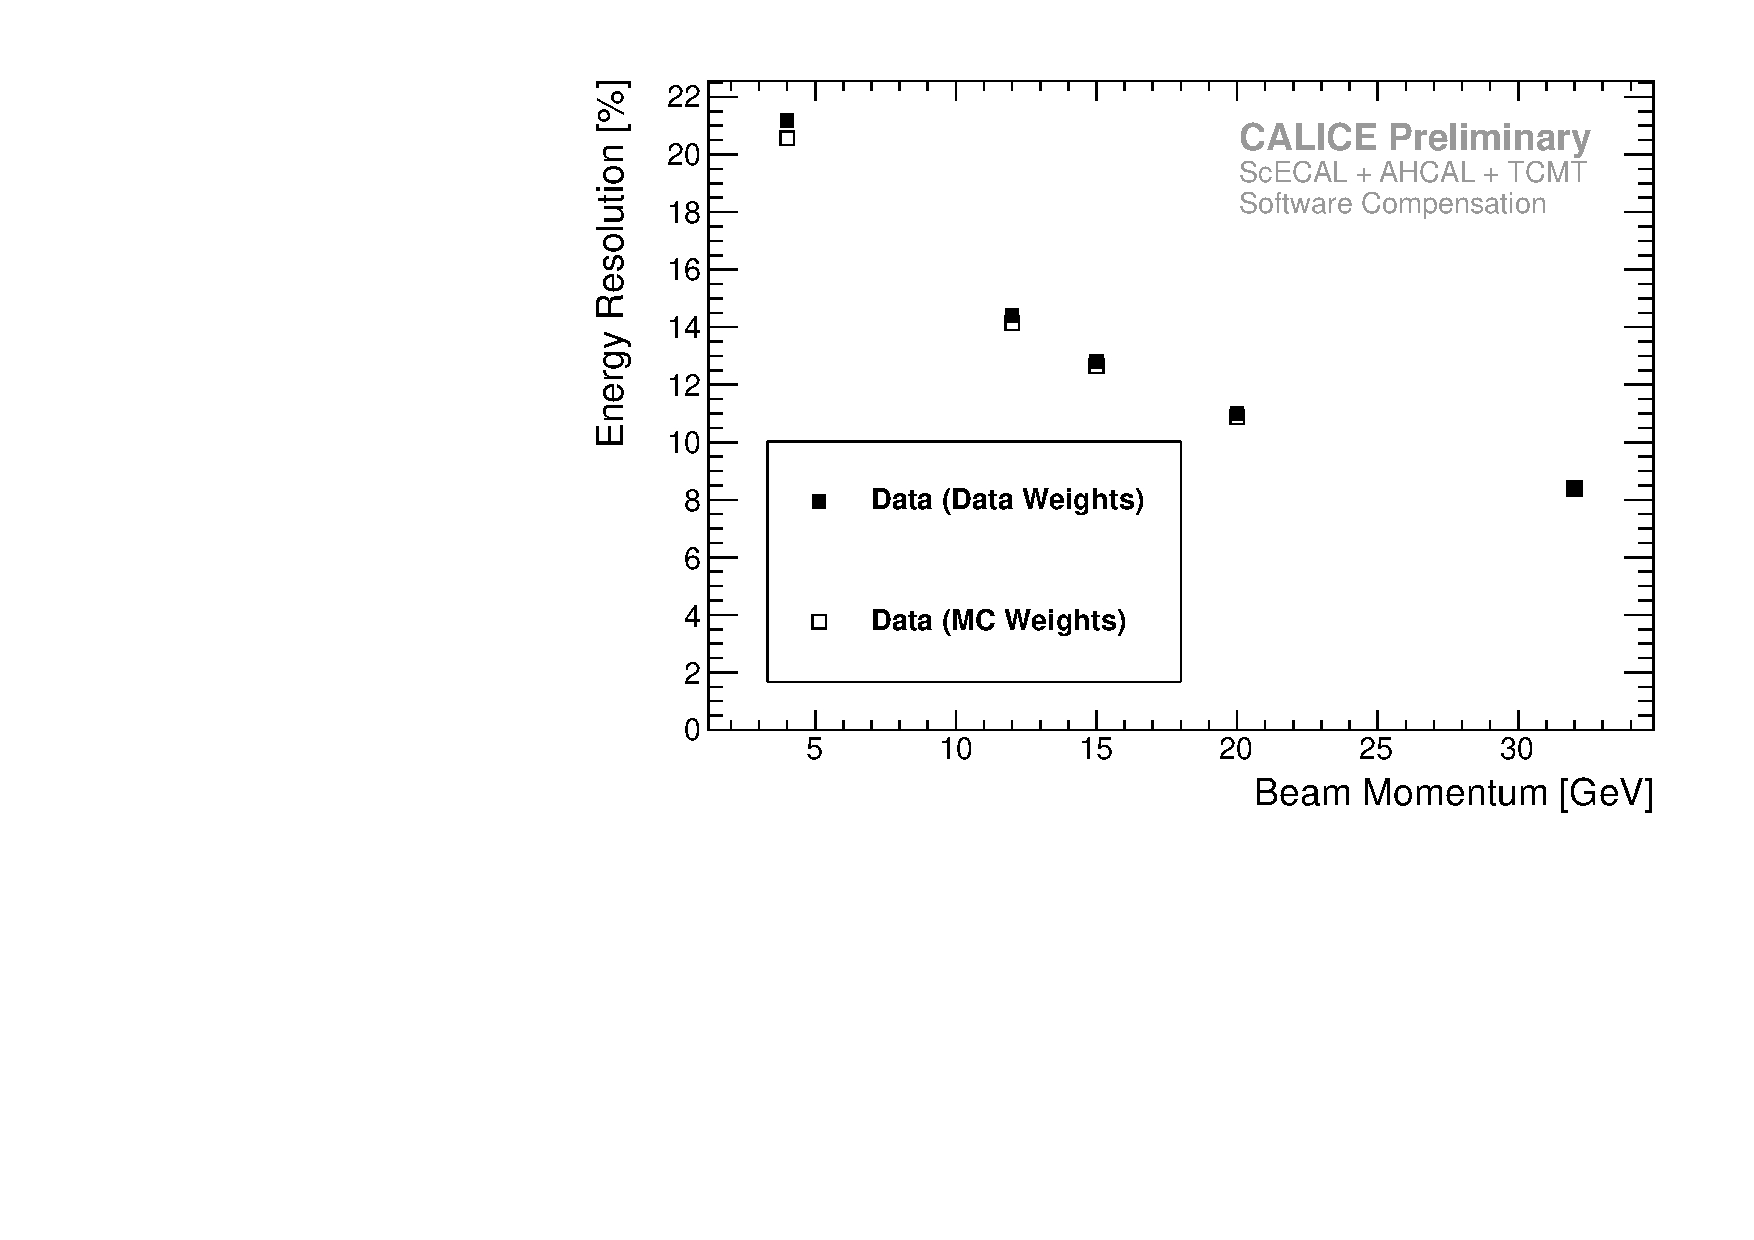
\includegraphics[width=0.5\textwidth]{fig/pion/results/pion_resolution_data_mc_weights}}\hfill
	\subfigure[Linearity Residual] {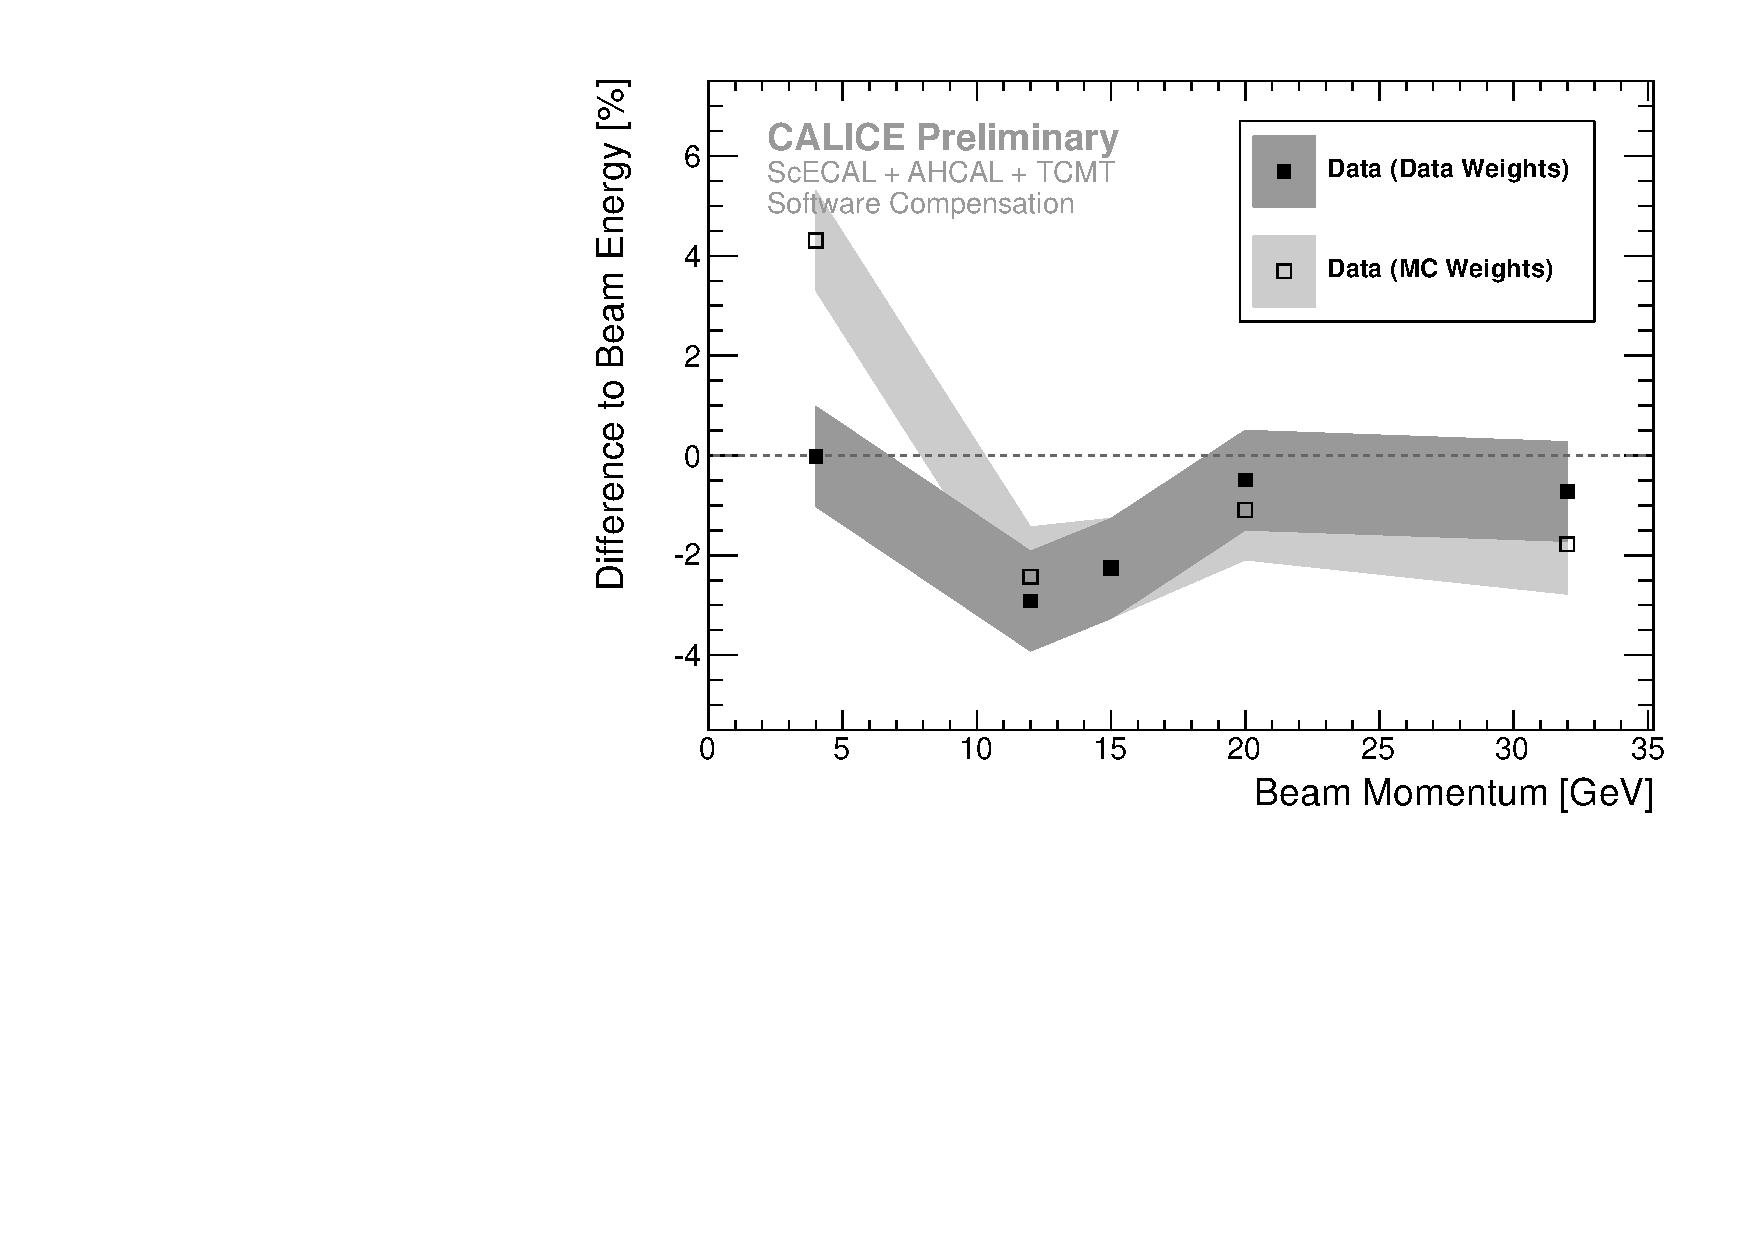
\includegraphics[width=0.5\textwidth]{fig/pion/results/pion_linearity_data_mc_weights}}
\end{center}
	\caption{Reconstructed energy resolution and linearity for the data sample when using software compensation weights derived from data and simulation (QGSP\_BERT\_HP in Geant\,4 10.2p1) for energy reconstruction. Reconstructing the data sample with software compensation weights derived from simulations, the energy resolution is marginally improved while the linearity is slightly deteriorated.}
	\label{fig:pion_data_mc_weights}
\end{figure}

\section{Summary}
This note presents results obtained with the combined scintillator-SiPM calorimeter system consisting of ScECAL, AHCAL and TCMT in the energy range 4--32\,GeV.

The simulation model of the ScECAL is validated with electromagnetic interactions from MIP signals in single cells up to full shower profiles. All observables show good agreement between data and simulation except for hit energy spectra which show differences in the high end tails. This is likely due to a combination of underestimated shower radii in simulation and imperfect saturation correction in data. The influence on pion measurements is expected to be small. Systematic uncertainties from these effects are propagated into the pion results.

Longitudinal profiles of pion showers show good agreement between data and simulation, with a general deposition overestimation of around 5\% in all tested simulation models. In the ScECAL the longitudinal shower profile as a function of distance to shower start shows considerable differences between simulation models, especially for high beam energies. 

Weights for standard energy reconstruction agree well in data and simulation apart from the generally overestimated depositions. The linearity deviation of pion energy reconstruction is \textless5\% in simulation and \textless3\% in data. The energy resolution of standard reconstruction is well described by all simulation models. 

The novel implementation of a local software compensation scheme does not enforce any functional dependence of weights between bins in hit energy density, while parametrising the dependence on particle energy. Counting hits instead of summing up depositions in the first two bins suppresses Landau fluctuations and slightly improves the energy resolution. The hit energy and beam energy dependent weights used for software compensation reconstruction are well described in the AHCAL. Significant discrepancies of these weights are observed in some ScECAL bins. This is potentially connected to, but not adequately explained by, the deviations in the hit energy spectra observed. The linearity deviation using software compensation reconstruction improves for data and simulation to \textless3\%. In data, the energy resolution improves by 10--20\% from applying software compensation. Energy resolution improvements from software compensation are overestimated in simulation by 5--10\% for all beam energies and simulation models.

Both standard and software compensation energy resolutions in data are in good agreement with resolutions obtained from a similar analysis in which only showers starting in the AHCAL are considered. The single pion energy resolution of the AHCAL is thus not altered by adding the ScECAL in front.

Applying the software compensation weights obtained from simulations to data runs results in practically identical performance numbers, slightly improving the achieved energy resolution while similarly slightly deteriorating the linearity. 
\clearpage

%\section{Acknowledgements}

\addcontentsline{toc}{section}{Bibliography}
\begin{thebibliography}{----------------}
\bibitem{Feege}
	N. Feege, Low-energetic hadron interactions in a highly granular calorimeter, \\
	DESY-THESIS-2011-048
\bibitem{CAN16}	
	CALICE Collaboration, K. Kotera, First Stage Analysis of the Energy Response and Resolution of the Scintillator ECAL in the Beam Test at FNAL, 2008 \\
	CALICE Analysis Note CAN-016
\bibitem{CommPaper}
	The CALICE collaboration, C. Adloff et al., Construction and Commissioning of the CALICE Analog Hadron Calorimeter Prototype\\
	2010 JINST 5 P05004\\
 	doi:10.1088/1748-0221/5/05/P05004
\bibitem{TCMTPaper}
	The CALICE collaboration, C. Adloff et al., Construction and performance of a silicon photomultiplier/extruded scintillator tail-catcher and muon-tracker\\
	2012 JINST 7 P04015\\
 	doi:10.1088/1748-0221/7/04/P04015
\bibitem{Guenter}
	C. G\"unter, Comparison of Iron and Tungsten Absorber Structures for an Analog Hadron Calorimeter, \\
	DESY-THESIS-2015-018
\bibitem{CAN16b}	
	CALICE Collaboration, K. Kotera, Update of the Analysis of the Test Beam Experiment of the CALICE ScECAL Physics Prototype\\
	CALICE Analysis Note CAN-016b
\bibitem{ScECALAbsorber}	
	K. Kotera, Tungsten Absorber for the CALICE ScECAL Prototype\\
	Internal Technical Note
\bibitem{EMPaper}
	The CALICE Collaboration, C. Adloff et al., Electromagnetic response of a highly granular hadronic calorimeter\\
	2011 JINST 6 P04003 \\
	doi:10.1088/1748-0221/6/04/P04003
\bibitem{SiPMNLO}	
	K. Kotera, W. Choi, T. Takeshita, SiPM Response Functions Representing Wide Range Including Linear Behavior After Saturation\\
	 \href{http://arxiv.org/abs/1510.01102}{arXiv:1510.01102 [physics.ins-det]}
\bibitem{FTBF}
	FTBF Website, \\
	\href{http://ftbf.fnal.gov/beam-delivery-path/}{http://ftbf.fnal.gov/beam\-delivery\-path/}
\bibitem{MarinaFHI}
	The CALICE Collaboration, Pion and proton showers in the CALICE scintillator-steel analogue hadron calorimeter, \\
	2015 JINST 10 P04014\\
	doi:10.1088/1748-0221/10/04/P04014
\bibitem{TrackSegments}
	The CALICE Collaboration, C. Adloff et al., Track segments in hadronic showers in a highly granular scintillator-steel hadron calorimeter, \\
	2013 JINST 8 P09001\\
	doi:10.1088/1748-0221/8/09/P09001
\bibitem{SCPaper}
	CALICE Collaboration, C. Adloff et al., Hadronic energy resolution of a highly granular scintillator-steel calorimeter using software compensation techniques\\
	2012  JINST 7 P09017 \\
	doi:10.1088/1748-0221/7/09/P09017
\bibitem{SDHCAL}	
	CALICE Collaboration, First results of the CALICE SDHCAL technological prototype \\
	2016 JINST 11 P04001\\
	doi:10.1088/1748-0221/11/04/P04001
\bibitem{CAN48}	
	CALICE Collaboration, M. Chadeeva, Parametrisation of hadron shower profiles in the CALICE Sc-Fe AHCAL\\
	CALICE Analysis Note CAN-048
\bibitem{CAN49}	
	CALICE Collaboration, C. Neub\"user, Analogue, Digital and Semi-Digital Energy Reconstruction in the CALICE AHCAL\\
	CALICE Analysis Note CAN-049

\bibitem{Marina}
	CALICE Collaboration, Pion and proton showers in the CALICE scintillator-steel AHCAL: comparison of global observables\\
	CALICE Analysis Note CAN-040
\bibitem{CAN16a}	
	CALICE Collaboration, A. Khan, Temperature Correction on ADC/MIP Conversion Factors for September 2009 Data of ScECAL FNAL Test Beam Module \\
	CALICE Analysis Note CAN-016a




	
\end{thebibliography}

\clearpage
\begin{appendix} 
\section*{Appendix}
\pagestyle{plain} 
%\setcounter{table}{0}
\renewcommand{\thetable}{A\arabic{table}}
\addcontentsline{toc}{section}{Appendix}

\begin{table}[htbp]
\begin{center}
\caption{Cuts applied to select single electrons. Cuts marked with $^{(\ast)}$ are applied only on data, cuts marked with $^{(\dagger)}$ are applied only on simulated events.}
\label{table:electronselection}
\begin{tabular}{l|r|>{\centering\arraybackslash}p{8.5cm}}
    \multicolumn{1}{c|}{Name} & \multicolumn{1}{c|}{Beam Energy} & \multicolumn{1}{c}{Cut} \\\hline
	\multirow{2}{*}{Raw}& All & beamBit = 1 $^{(\ast)}$\\
	& All & a10x10Bit = 1 $^{(\dagger)}$\\\hline
	\multirow{5}{*}{Event Quality}& All & vetoBit = 0 $^{(\ast)}$\\
	& All & 2000 \textless multiADC \textless 3800 $^{(\ast)}$\\
	& All & Energy in first 5 ScECAL layers \textgreater 3.5\,MIP \\
	& All & cherenkowBit = 0 $^{(\ast)}$\\
	& All & cherenkow2Bit = 1 $^{(\ast)}$\\\hline
	\multirow{2}{*}{Electron Selection} & All & reconstructed FHI layer $\leq$ 4\\
	& All & $\frac{E_\text{sum}^\text{ScECAL}}{E_\text{sum}^\text{ScECAL} + E_\text{sum}^\text{AHCAL}}> 0.9$\\	
	& \multirow{2}{*}{All} & (nHits$^\text{AHCAL}$\textless35 $\|$ nHits$^\text{AHCAL}$\textgreater65) \&\&
(cog$_\text{Z}^\text{AHCAL}$\textless\ 2000\,mm $\|$ cog$_\text{Z}^\text{AHCAL}$\textgreater\ 2250\,mm) \\\hline
	\multirow{2}{*}{Multi Particle Suppr.} & All & nTracks in AHCAL = 0\\
	& All & nTracks (isolated) in ScECAL = 0\\\hline
	
	Containment & All & shower CoG in central quarter of the ScECAL\\
	
	
\end{tabular}
\end{center}
\end{table}

\begin{table}[htbp]
\begin{center}
\caption{Cuts applied to select single pions. Cuts marked with $^{(\ast)}$ are applied only on data, cuts marked with $^{(\dagger)}$ are applied only on simulated events.}
\label{table:pionselection}
\begin{tabular}{l|r|>{\centering\arraybackslash}p{8.5cm}}
    \multicolumn{1}{c|}{Name} & \multicolumn{1}{c|}{Beam Energy} & \multicolumn{1}{c}{Cut} \\\hline
	\multirow{2}{*}{Raw}& All & beamBit = 1 $^{(\ast)}$\\
	& All & a10x10Bit = 1 $^{(\dagger)}$\\\hline
	\multirow{5}{*}{Event Quality}& All & vetoBit = 0 $^{(\ast)}$\\
	& All & 2000 \textless multiADC \textless 3800 $^{(\ast)}$\\
	& All & Energy in first 5 ScECAL layers \textgreater 3.5\,MIP \\
	& $\leq$4\,GeV & cherenkowBit = 0 $^{(\ast)}$\\
	& $\leq$4\,GeV & cherenkow2Bit = 0 $^{(\ast)}$\\\hline
	\multirow{2}{*}{Pion Selection} & All & reconstructed FHI layer $\geq$ 5\\	
	& \multirow{2}{*}{All} & (nHits$^\text{AHCAL}$\textless35 $\|$ nHits$^\text{AHCAL}$\textgreater65) \&\&
(cog$_\text{Z}^\text{AHCAL}$\textless\ 2000\,mm $\|$ cog$_\text{Z}^\text{AHCAL}$\textgreater\ 2250\,mm) \\\hline
	\multirow{2}{*}{Multi Particle Suppr.} & All & nTracks parallel to beam in outer AHCAL = 0\\
	& All & nTracks (isolated) in ScECAL = 1\\\hline
	\multirow{2}{*}{Containment} & All & reconstructed FHI layer $\leq$ 35\\
	& All & isolated track in central quarter of ScECAL\\
	
\end{tabular}
\end{center}
\end{table}

\begin{table}[htbp]
\begin{center}
\caption{Selection efficiencies and response/resolution biases for minimal and full pion selection for different physics list and particle types. The \emph{FHI} sample is selected for scintillator trigger and FHI layer cuts only, \emph{sel.} contains the full pion selection as decribed in \ref{sec:pionselection}. The efficiency $\epsilon_\text{sel.}$ is given as the fraction of events that pass the full pion selection out of all events that hit the trigger scintillator (\emph{raw cut}). Statistical errors on fit are negligibly small. \emph{Raw} samples have around 100,000 events each, with only around 50,000 events at 4\,GeV beam energy. All simulations are done with \geant\ 10.1p2 except lines marked with\ $^{(\ast)}$, which are \geant 9.6p3. }
\label{table:pionselectionMC}
\begin{tabular}{p{1.8cm}c|l|r|r|r|r|r}
	\multicolumn{2}{c|}{Run/Particle} & \multicolumn{1}{c|}{Physics List} & \multicolumn{1}{c|}{$\nicefrac{\mu_\text{FHI}}{\text{GeV}}$} & \multicolumn{1}{c|}{$\nicefrac{\sigma_\text{FHI}}{\mu_\text{FHI}}$} & \multicolumn{1}{c|}{$\nicefrac{\mu_\text{sel.}}{\text{GeV}}$} & \multicolumn{1}{c|}{$\nicefrac{\sigma_\text{sel.}}{\mu_\text{sel.}}$}  & \multicolumn{1}{c}{$\epsilon_\text{sel.}$} \\\hline
   
	\multirow{4}{*}{\begin{minipage}{1.8cm}\centering 560506\\ (4\,GeV)\end{minipage} }	& \piminus	&\footnotesize{FTFP\_BERT\_HP} 			& 3.82	& 22.92\%	& 3.83 & 22.86\% & 46.1\% \\
												& \piminus	&\footnotesize{FTFP\_BERT\_HP$^{(\ast)}$}	& 3.81	& 22.64\%	& 3.82 & 22.59\% & 46.5\% \\
												& \piminus	&\footnotesize{QGSP\_BERT\_HP} 			& 3.80	& 22.95\%	& 3.81 & 22.87\% & 45.9\% \\
												& \eminus	&\footnotesize{QGSP\_BERT} 			& - 	& - & - & - & 0.2\% \\\hline
	\multirow{4}{*}{\begin{minipage}{1.8cm}\centering 560498\\ (12\,GeV)\end{minipage} }	& \piminus	&\footnotesize{FTFP\_BERT\_HP} 			& 11.62	& 15.49\% & 11.67 & 15.37\% & 49.5\%\\
												& \piminus	&\footnotesize{FTFP\_BERT\_HP$^{(\ast)}$}	& 11.68	& 14.73\% & 11.71 & 14.65\% & 49.6\%\\
												& \piminus	&\footnotesize{QGSP\_BERT\_HP} 			& 11.54	& 15.54\% & 11.59 & 15.45\% & 49.4\%\\
												& \eminus	&\footnotesize{QGSP\_BERT} 			& - 	& - & - & - & \textless 0.1\% \\\hline
	\multirow{4}{*}{\begin{minipage}{1.8cm}\centering 560496\\ (15\,GeV)\end{minipage} }	& \piminus	&\footnotesize{FTFP\_BERT\_HP} 			& 14.64	& 14.43\%	& 14.70 & 14.30\% & 48.8\%\\
												& \piminus	&\footnotesize{FTFP\_BERT\_HP$^{(\ast)}$}	& 14.69	& 13.59\%	& 14.74 & 13.49\% & 49.1\%\\
												& \piminus	&\footnotesize{QGSP\_BERT\_HP} 			& 14.66	& 14.30\%	& 14.71 & 14.20\% & 49.2\%\\
												& \eminus	&\footnotesize{QGSP\_BERT} 			& - 	& - & - & - & \textless 0.1\% \\\hline
	\multirow{4}{*}{\begin{minipage}{1.8cm}\centering 560481\\ (20\,GeV)\end{minipage} }	& \piminus	&\footnotesize{FTFP\_BERT\_HP} 			& 19.69	& 13.25\%	& 19.78 & 13.19\% & 47.5\%\\
												& \piminus	&\footnotesize{FTFP\_BERT\_HP$^{(\ast)}$}	& 19.70	& 12.35\%	& 19.77 & 12.28\% & 47.6\%\\
												& \piminus	&\footnotesize{QGSP\_BERT\_HP} 			& 19.78	& 12.74\%	& 19.86 & 12.66\% & 48.0\%\\
												& \eminus	&\footnotesize{QGSP\_BERT} 			& - 	& - 		& - 	& - 	& \textless 0.1\% \\\hline
	\multirow{4}{*}{\begin{minipage}{1.8cm}\centering 560474\\ (32\,GeV)\end{minipage} }	& \piminus	&\footnotesize{FTFP\_BERT\_HP} 			& 31.97	& 11.59\%	& 32.15 & 11.58\% & 44.3\%\\
												& \piminus	&\footnotesize{FTFP\_BERT\_HP$^{(\ast)}$}	& 31.97	& 10.66\%	& 32.12 & 10.60\% & 44.3\%\\
												& \piminus	&\footnotesize{QGSP\_BERT\_HP} 			& 31.92	& 10.96\%	& 32.08 & 10.82\% & 45.0\%\\
												& \eminus	&\footnotesize{QGSP\_BERT} 			& - 	& - 		& - & - & \textless 0.1\% \\
\end{tabular}
\end{center}
\end{table}

\begin{table}[htbp]
\begin{center}
\caption{Energy resolutions extracted from pion runs in data and simulations, using the standard energy reconstruction (Std.) and the software compensation reconstruction (SC) as plotted in \autoref{fig:pion_resolution_plots}. Errors on data are purely statistical, errors on simulation include systematic modelling uncertainties. All simulations are generated with GEANT\,4 10.1p2 except lines marked with\ $^{(\ast)}$, which are GEANT\,4 9.6p3. }
\label{table:pionresolution}
\begin{tabular}{p{1.8cm}c|l|c|c|c}
\multicolumn{2}{c|}{Run/Particle} & \multicolumn{1}{c|}{Type}	& \multicolumn{1}{c|}{$\left(\nicefrac{\sigma}{\mu}\right)_\text{Std.} \left[\%\right]$} & \multicolumn{1}{c|}{$\left(\nicefrac{\sigma}{\mu}\right)_\text{SC} \left[\%\right]$}& \multicolumn{1}{c}{$\frac{\left(\nicefrac{\sigma}{\mu}\right)_\text{SC}}{\left(\nicefrac{\sigma}{\mu}\right)_\text{Std.}} $}\\
	\hline
	\multirow{4}{*}{\begin{minipage}{1.8cm}\centering 560506\\ (4\,GeV)\end{minipage} }	& \piminus	&\footnotesize{Data} 				& 23.30 $\pm$ 0.08 & 21.19 $\pm$ 0.07 & 0.91 $\pm$ 0.00 \\
												& \piminus	&\footnotesize{FTFP\_BERT\_HP} 			 & 22.56 $\pm$ 0.65 & 19.00 $\pm$ 0.39 & 0.84 $\pm$ 0.03 \\
												& \piminus	&\footnotesize{FTFP\_BERT\_HP$^{(\ast)}$}	 & 22.86 $\pm$ 0.81 & 19.57 $\pm$ 0.57 & 0.86 $\pm$ 0.04 \\
												& \piminus	&\footnotesize{QGSP\_BERT\_HP} 			 & 22.85 $\pm$ 0.78 & 19.51 $\pm$ 0.56 & 0.85 $\pm$ 0.04 \\
	\hline
	\multirow{4}{*}{\begin{minipage}{1.8cm}\centering 560498\\ (12\,GeV)\end{minipage} }	& \piminus	&\footnotesize{Data} 				& 15.98 $\pm$ 0.05 & 14.40 $\pm$ 0.05 & 0.90 $\pm$ 0.00 \\
												& \piminus	&\footnotesize{FTFP\_BERT\_HP} 			 & 14.65 $\pm$ 0.25 & 12.60 $\pm$ 0.20 & 0.86 $\pm$ 0.02 \\
												& \piminus	&\footnotesize{FTFP\_BERT\_HP$^{(\ast)}$}	& 15.38 $\pm$ 0.28 & 12.79 $\pm$ 0.32 & 0.83 $\pm$ 0.03 \\
												& \piminus	&\footnotesize{QGSP\_BERT\_HP} 			& 15.45 $\pm$ 0.29 & 12.69 $\pm$ 0.25 & 0.82 $\pm$ 0.02 \\
	\hline
	\multirow{4}{*}{\begin{minipage}{1.8cm}\centering 560496\\ (15\,GeV)\end{minipage} }	& \piminus	&\footnotesize{Data} 				& 14.59 $\pm$ 0.04 & 12.81 $\pm$ 0.04 & 0.88 $\pm$ 0.00 \\
												& \piminus	&\footnotesize{FTFP\_BERT\_HP} 			& 13.50 $\pm$ 0.30 & 11.31 $\pm$ 0.20 & 0.84 $\pm$ 0.02 \\
												& \piminus	&\footnotesize{FTFP\_BERT\_HP$^{(\ast)}$}	& 14.32 $\pm$ 0.37 & 11.45 $\pm$ 0.33 & 0.80 $\pm$ 0.03 \\
												& \piminus	&\footnotesize{QGSP\_BERT\_HP} 			& 14.20 $\pm$ 0.20 & 11.38 $\pm$ 0.13 & 0.80 $\pm$ 0.01 \\
	\hline
	\multirow{4}{*}{\begin{minipage}{1.8cm}\centering 560481\\ (20\,GeV)\end{minipage} }	& \piminus	&\footnotesize{Data} 				& 13.03 $\pm$ 0.04 & 10.99 $\pm$ 0.04 & 0.84 $\pm$ 0.00 \\
												& \piminus	&\footnotesize{FTFP\_BERT\_HP} 			& 12.29 $\pm$ 0.19 & 9.89 $\pm$ 0.22 & 0.80 $\pm$ 0.02 \\
												& \piminus	&\footnotesize{FTFP\_BERT\_HP$^{(\ast)}$}	& 13.19 $\pm$ 0.28 & 9.99 $\pm$ 0.28 & 0.76 $\pm$ 0.03 \\
												& \piminus	&\footnotesize{QGSP\_BERT\_HP} 			& 12.67 $\pm$ 0.13 & 9.76 $\pm$ 0.08 & 0.77 $\pm$ 0.01 \\
	\hline
	\multirow{4}{*}{\begin{minipage}{1.8cm}\centering 560474\\ (32\,GeV)\end{minipage} }	& \piminus	&\footnotesize{Data} 				& 10.77 $\pm$ 0.03 & 8.36 $\pm$ 0.02 & 0.78 $\pm$ 0.00 \\
												& \piminus	&\footnotesize{FTFP\_BERT\_HP} 			& 10.62 $\pm$ 0.20 & 7.52 $\pm$ 0.13 & 0.71 $\pm$ 0.02 \\
												& \piminus	&\footnotesize{FTFP\_BERT\_HP$^{(\ast)}$}	& 11.59 $\pm$ 0.28 & 7.61 $\pm$ 0.03 & 0.66 $\pm$ 0.02 \\
												& \piminus	&\footnotesize{QGSP\_BERT\_HP} 			& 10.84 $\pm$ 0.22 & 7.56 $\pm$ 0.13 & 0.70 $\pm$ 0.02 \\
\end{tabular}
\end{center}
\end{table}

\clearpage
\begin{figure}[t]
\begin{center}
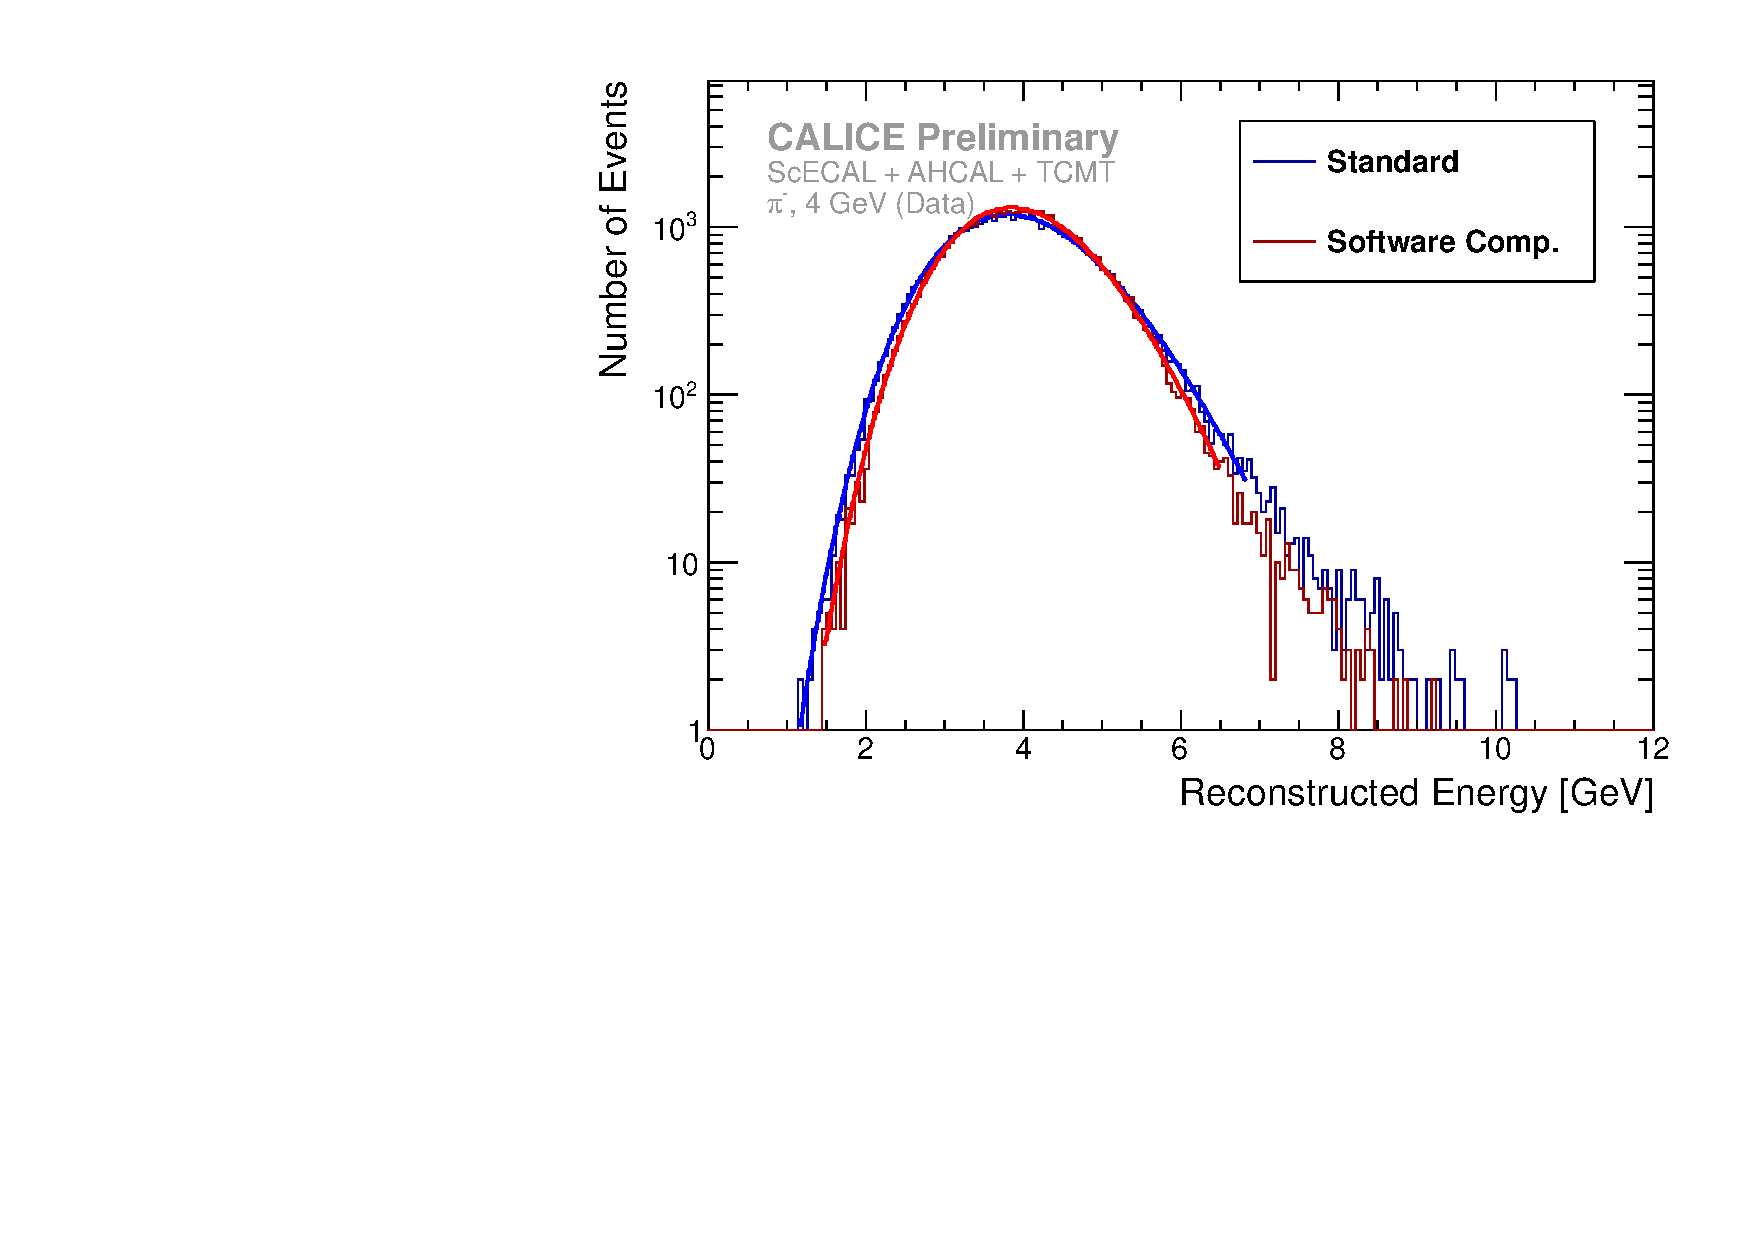
\includegraphics[width=0.8\textwidth]{fig/pion/SC/ERec_classic_SC_560506_data.pdf}
\caption{Reconstructed energy spectrum in standard and software compensation reconstruction for data run 560506 (4\,GeV \piminus).}
\label{fig:erec_pi_4gev}
\end{center}
\end{figure}

\begin{figure}[b]
\begin{center}
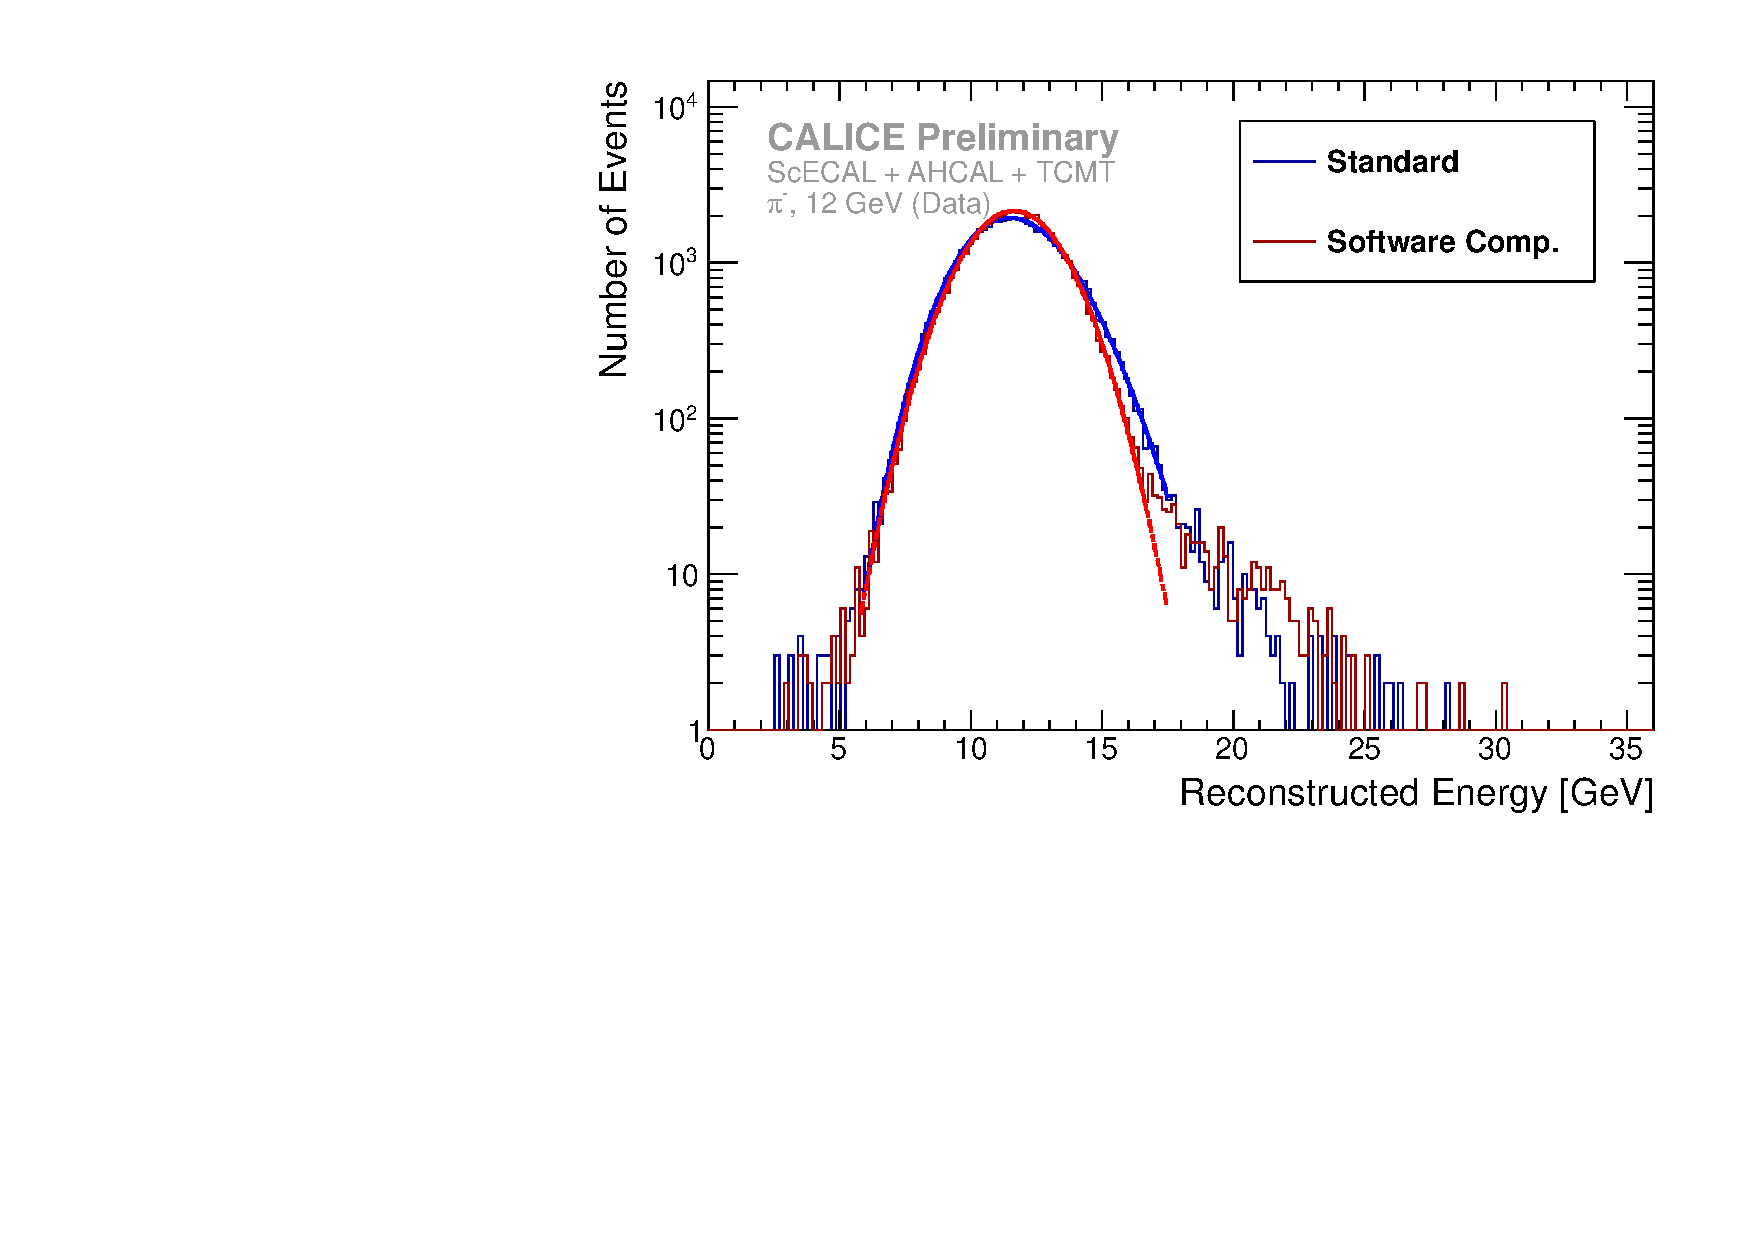
\includegraphics[width=0.8\textwidth]{fig/pion/SC/ERec_classic_SC_560498_data.pdf}
\caption{Reconstructed energy spectrum in standard and software compensation reconstruction for data run 560498 (12\,GeV \piminus).}
\label{fig:erec_pi_12gev}
\end{center}
\end{figure}

\begin{figure}[t]
\begin{center}
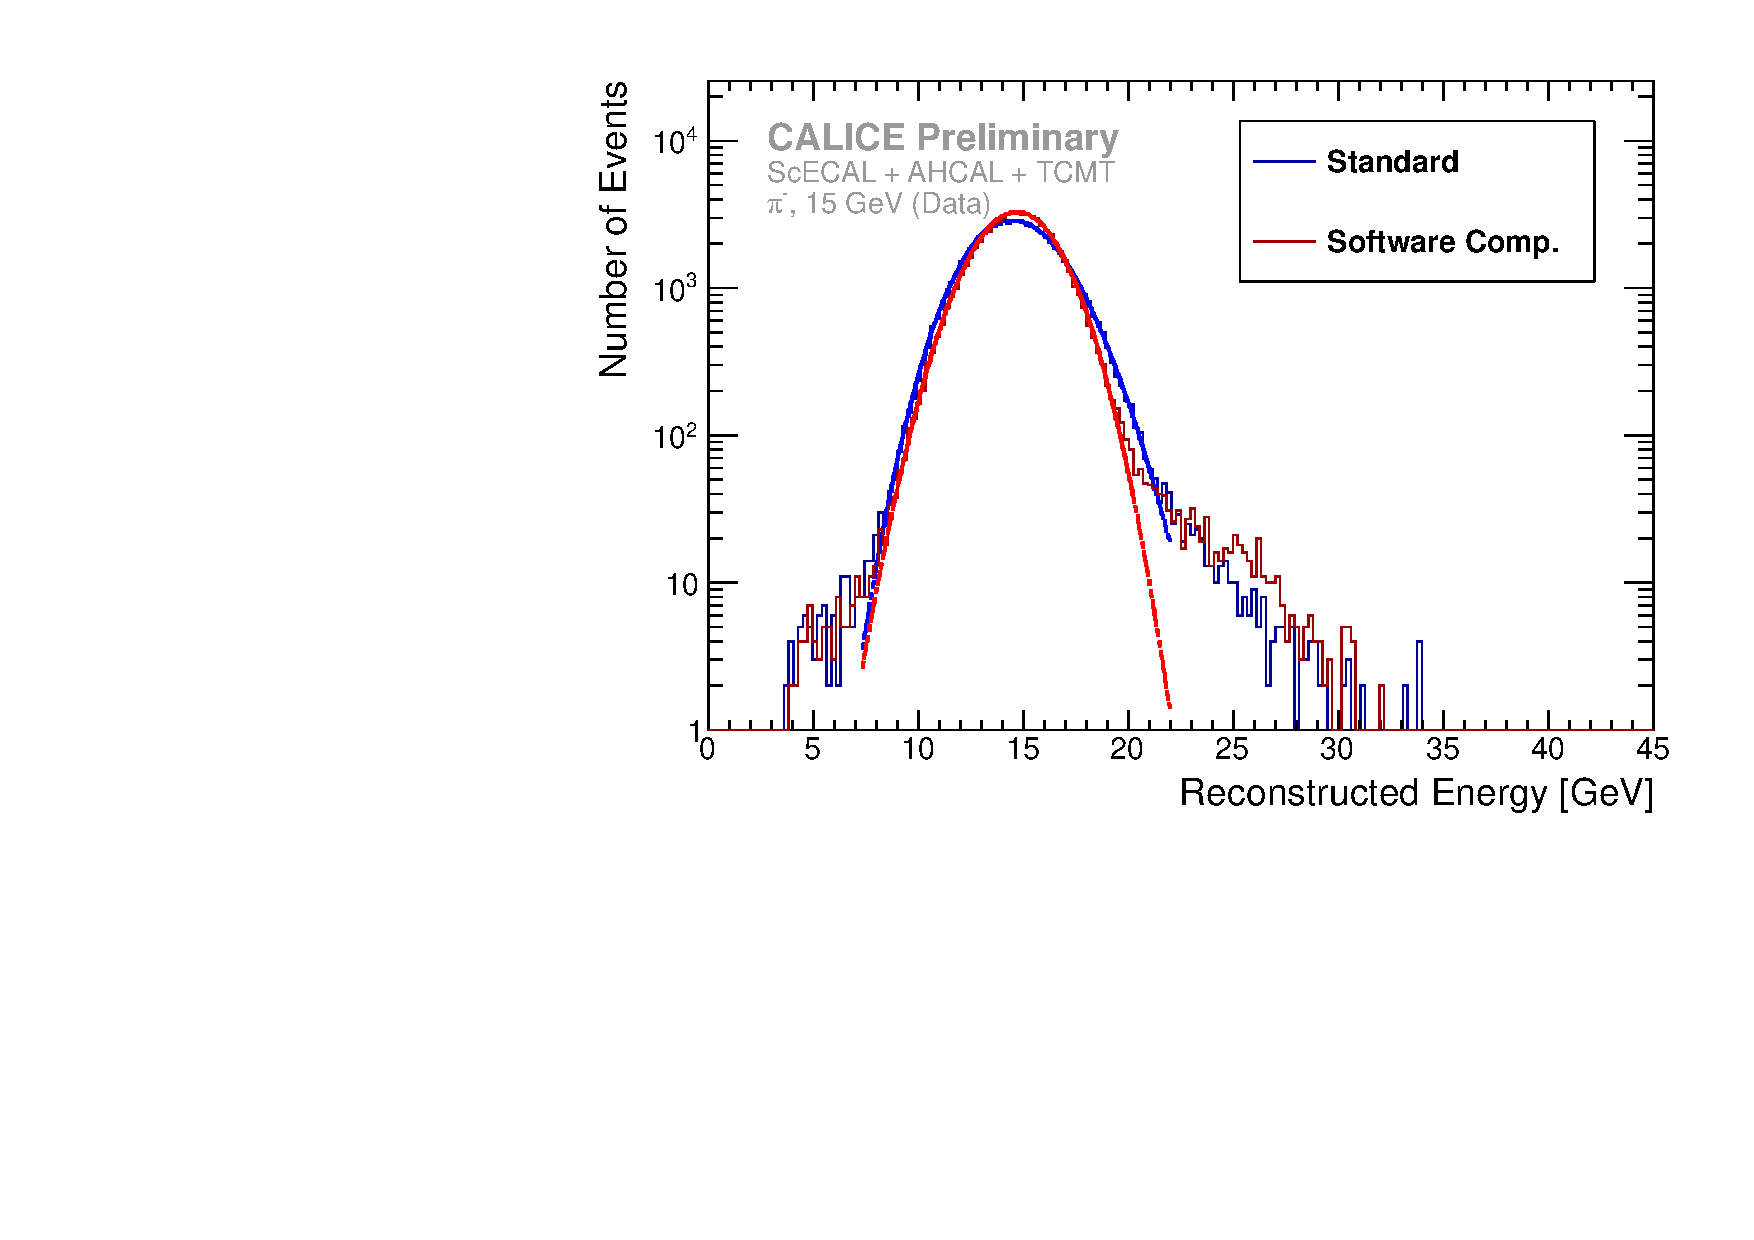
\includegraphics[width=0.8\textwidth]{fig/pion/SC/ERec_classic_SC_560496_data.pdf}
\caption{Reconstructed energy spectrum in standard and software compensation reconstruction for data run 560496 (15\,GeV \piminus).}
\label{fig:erec_pi_15gev}
\end{center}
\end{figure}

\begin{figure}[b]
\begin{center}
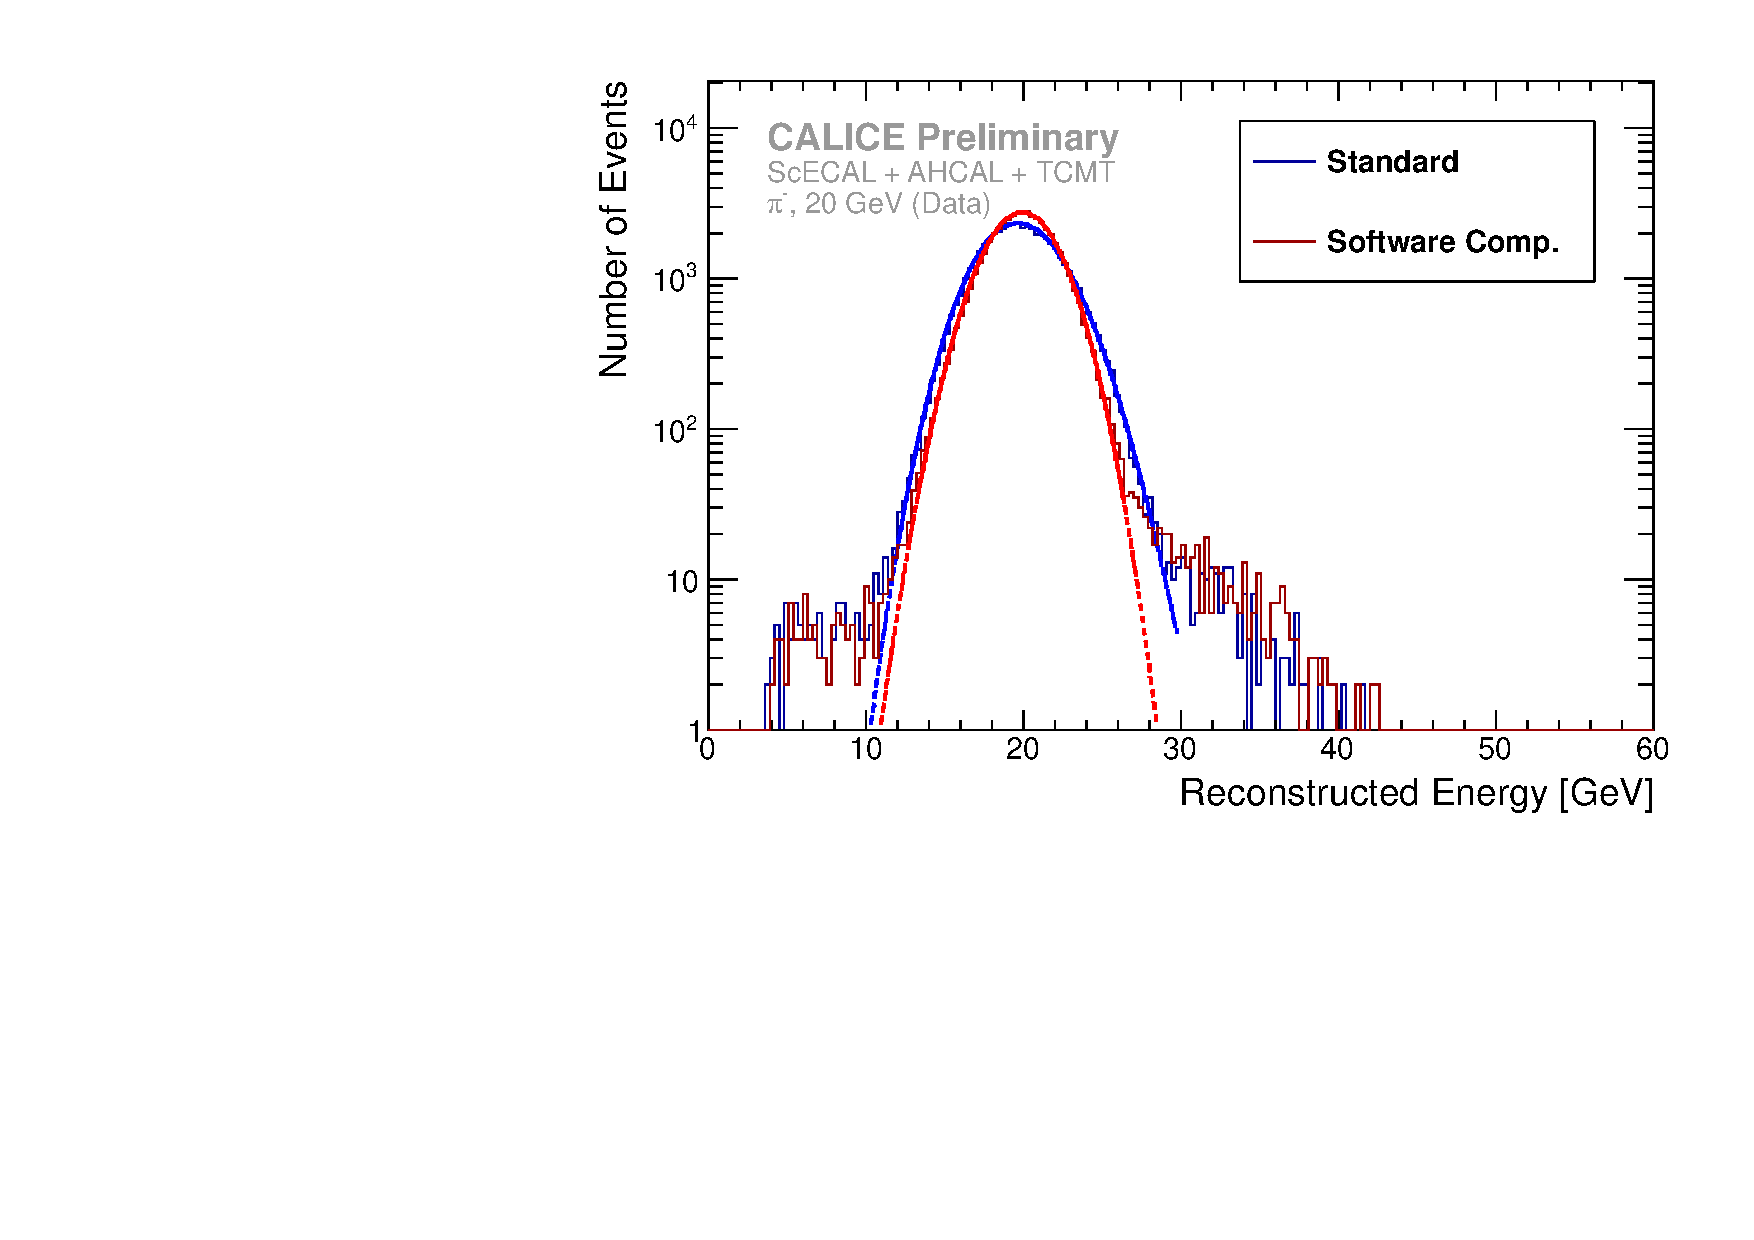
\includegraphics[width=0.8\textwidth]{fig/pion/SC/ERec_classic_SC_560481_data.pdf}
\caption{Reconstructed energy spectrum in standard and software compensation reconstruction for data run 560481 (20\,GeV \piminus).}
\label{fig:erec_pi_20gev}
\end{center}
\end{figure}

\begin{figure}[htbp]
\begin{center}
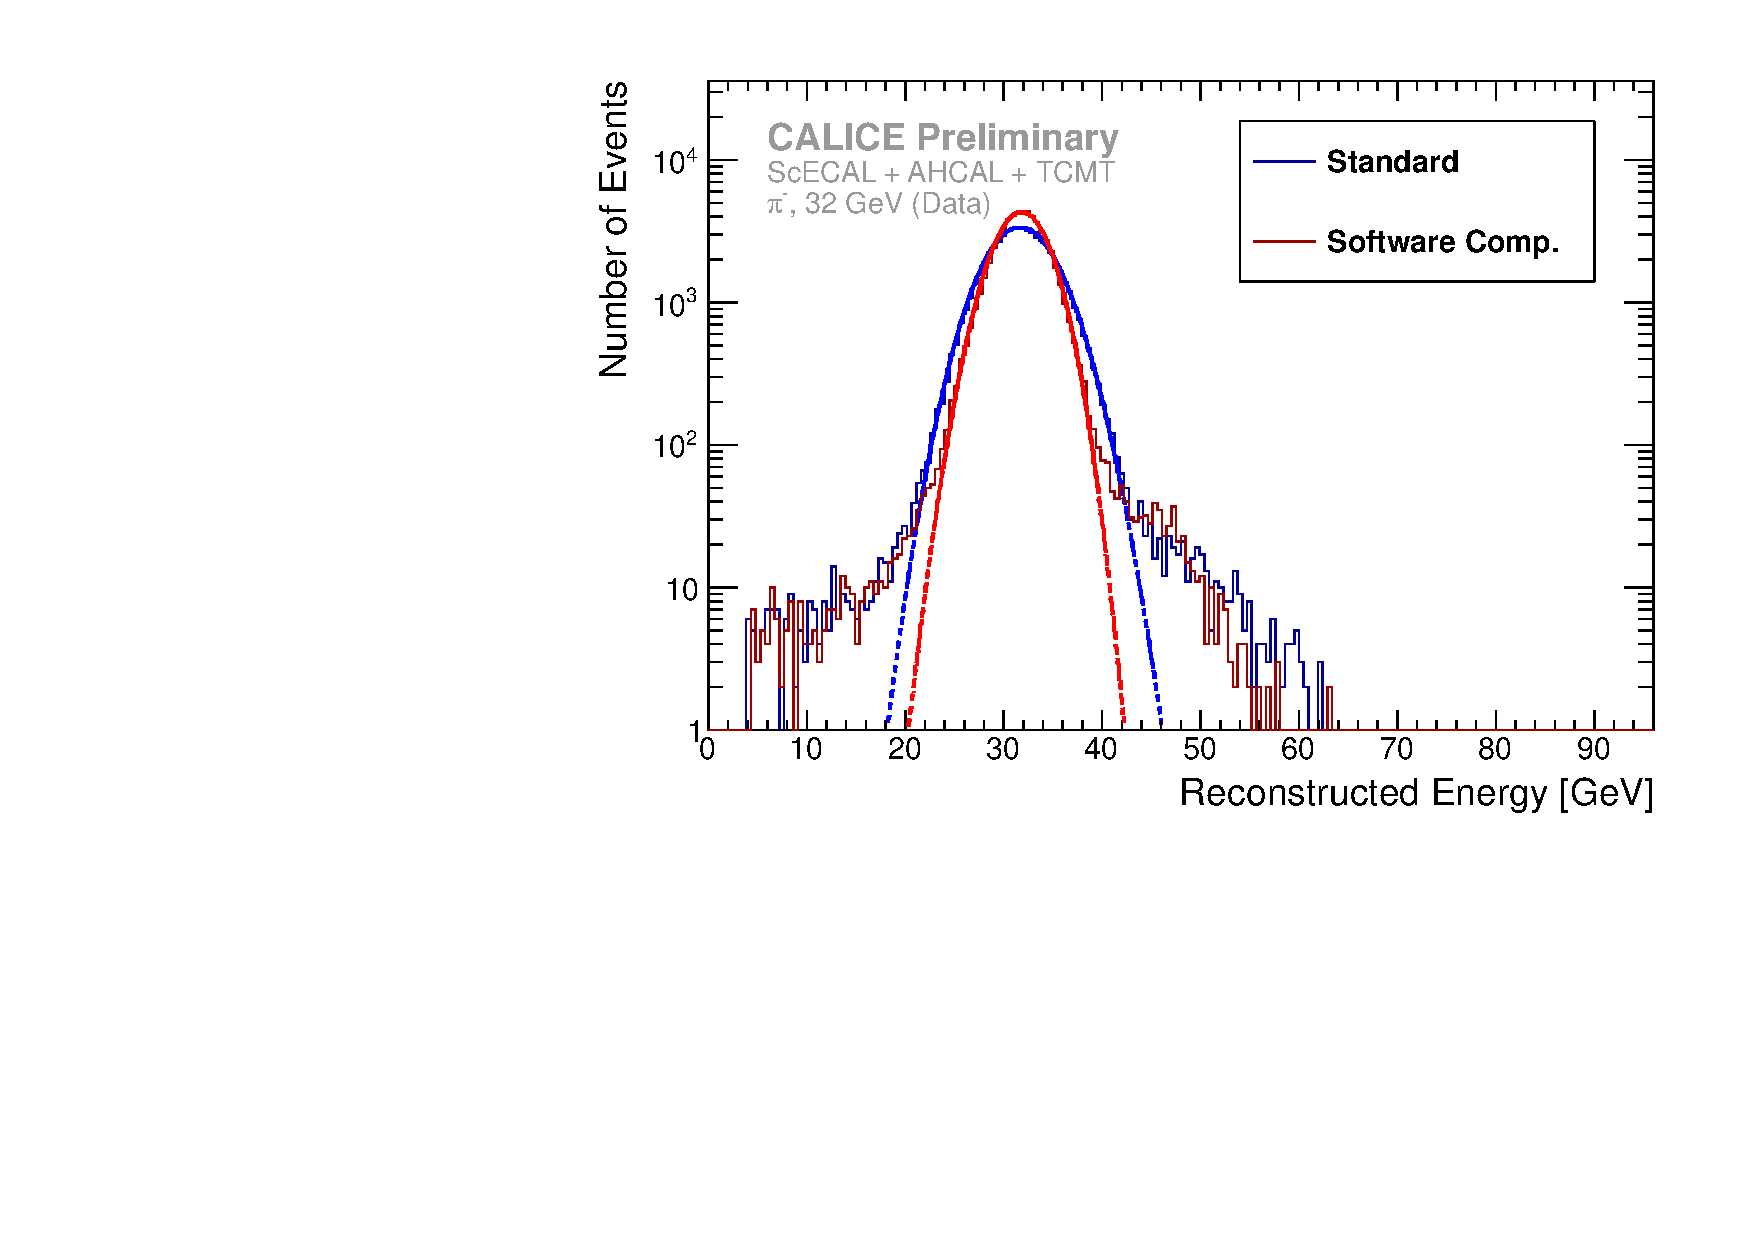
\includegraphics[width=0.8\textwidth]{fig/pion/SC/ERec_classic_SC_560474_data.pdf}
\caption{Reconstructed energy spectrum in standard and software compensation reconstruction for data run 560474 (32\,GeV \piminus).}
\label{fig:erec_pi_32gev}
\end{center}
\end{figure}

\end{appendix}
\end{document}
